\documentclass[twoside]{book}

% Packages required by doxygen
\usepackage{fixltx2e}
\usepackage{calc}
\usepackage{doxygen}
\usepackage{graphicx}
\usepackage[utf8]{inputenc}
\usepackage{makeidx}
\usepackage{multicol}
\usepackage{multirow}
\PassOptionsToPackage{warn}{textcomp}
\usepackage{textcomp}
\usepackage[nointegrals]{wasysym}
\usepackage[table]{xcolor}

% Font selection
\usepackage[T1]{fontenc}
\usepackage{mathptmx}
\usepackage[scaled=.90]{helvet}
\usepackage{courier}
\usepackage{amssymb}
\usepackage{sectsty}
\renewcommand{\familydefault}{\sfdefault}
\allsectionsfont{%
  \fontseries{bc}\selectfont%
  \color{darkgray}%
}
\renewcommand{\DoxyLabelFont}{%
  \fontseries{bc}\selectfont%
  \color{darkgray}%
}
\newcommand{\+}{\discretionary{\mbox{\scriptsize$\hookleftarrow$}}{}{}}

% Page & text layout
\usepackage{geometry}
\geometry{%
  a4paper,%
  top=2.5cm,%
  bottom=2.5cm,%
  left=2.5cm,%
  right=2.5cm%
}
\tolerance=750
\hfuzz=15pt
\hbadness=750
\setlength{\emergencystretch}{15pt}
\setlength{\parindent}{0cm}
\setlength{\parskip}{0.2cm}
\makeatletter
\renewcommand{\paragraph}{%
  \@startsection{paragraph}{4}{0ex}{-1.0ex}{1.0ex}{%
    \normalfont\normalsize\bfseries\SS@parafont%
  }%
}
\renewcommand{\subparagraph}{%
  \@startsection{subparagraph}{5}{0ex}{-1.0ex}{1.0ex}{%
    \normalfont\normalsize\bfseries\SS@subparafont%
  }%
}
\makeatother

% Headers & footers
\usepackage{fancyhdr}
\pagestyle{fancyplain}
\fancyhead[LE]{\fancyplain{}{\bfseries\thepage}}
\fancyhead[CE]{\fancyplain{}{}}
\fancyhead[RE]{\fancyplain{}{\bfseries\leftmark}}
\fancyhead[LO]{\fancyplain{}{\bfseries\rightmark}}
\fancyhead[CO]{\fancyplain{}{}}
\fancyhead[RO]{\fancyplain{}{\bfseries\thepage}}
\fancyfoot[LE]{\fancyplain{}{}}
\fancyfoot[CE]{\fancyplain{}{}}
\fancyfoot[RE]{\fancyplain{}{\bfseries\scriptsize Generated on Thu Jul 14 2016 03\+:35\+:32 for My Project by Doxygen }}
\fancyfoot[LO]{\fancyplain{}{\bfseries\scriptsize Generated on Thu Jul 14 2016 03\+:35\+:32 for My Project by Doxygen }}
\fancyfoot[CO]{\fancyplain{}{}}
\fancyfoot[RO]{\fancyplain{}{}}
\renewcommand{\footrulewidth}{0.4pt}
\renewcommand{\chaptermark}[1]{%
  \markboth{#1}{}%
}
\renewcommand{\sectionmark}[1]{%
  \markright{\thesection\ #1}%
}

% Indices & bibliography
\usepackage{natbib}
\usepackage[titles]{tocloft}
\setcounter{tocdepth}{3}
\setcounter{secnumdepth}{5}
\makeindex

% Hyperlinks (required, but should be loaded last)
\usepackage{ifpdf}
\ifpdf
  \usepackage[pdftex,pagebackref=true]{hyperref}
\else
  \usepackage[ps2pdf,pagebackref=true]{hyperref}
\fi
\hypersetup{%
  colorlinks=true,%
  linkcolor=blue,%
  citecolor=blue,%
  unicode%
}

% Custom commands
\newcommand{\clearemptydoublepage}{%
  \newpage{\pagestyle{empty}\cleardoublepage}%
}


%===== C O N T E N T S =====

\begin{document}

% Titlepage & ToC
\hypersetup{pageanchor=false,
             bookmarks=true,
             bookmarksnumbered=true,
             pdfencoding=unicode
            }
\pagenumbering{roman}
\begin{titlepage}
\vspace*{7cm}
\begin{center}%
{\Large My Project }\\
\vspace*{1cm}
{\large Generated by Doxygen 1.8.8}\\
\vspace*{0.5cm}
{\small Thu Jul 14 2016 03:35:32}\\
\end{center}
\end{titlepage}
\clearemptydoublepage
\tableofcontents
\clearemptydoublepage
\pagenumbering{arabic}
\hypersetup{pageanchor=true}

%--- Begin generated contents ---
\chapter{L\+I\+C\+E\+N\+C\+E}
\label{md_LICENCE}
\hypertarget{md_LICENCE}{}
G\+N\+U G\+E\+N\+E\+R\+A\+L P\+U\+B\+L\+I\+C L\+I\+C\+E\+N\+S\+E Version 3, 29 June 2007

Copyright (C) 2007 Free Software Foundation, Inc. \href{http://fsf.org/}{\tt http\+://fsf.\+org/} Everyone is permitted to copy and distribute verbatim copies of this license document, but changing it is not allowed. \begin{DoxyVerb}                       Preamble
\end{DoxyVerb}


The G\+N\+U General Public License is a free, copyleft license for software and other kinds of works.

The licenses for most software and other practical works are designed to take away your freedom to share and change the works. By contrast, the G\+N\+U General Public License is intended to guarantee your freedom to share and change all versions of a program--to make sure it remains free software for all its users. We, the Free Software Foundation, use the G\+N\+U General Public License for most of our software; it applies also to any other work released this way by its authors. You can apply it to your programs, too.

When we speak of free software, we are referring to freedom, not price. Our General Public Licenses are designed to make sure that you have the freedom to distribute copies of free software (and charge for them if you wish), that you receive source code or can get it if you want it, that you can change the software or use pieces of it in new free programs, and that you know you can do these things.

To protect your rights, we need to prevent others from denying you these rights or asking you to surrender the rights. Therefore, you have certain responsibilities if you distribute copies of the software, or if you modify it\+: responsibilities to respect the freedom of others.

For example, if you distribute copies of such a program, whether gratis or for a fee, you must pass on to the recipients the same freedoms that you received. You must make sure that they, too, receive or can get the source code. And you must show them these terms so they know their rights.

Developers that use the G\+N\+U G\+P\+L protect your rights with two steps\+: (1) assert copyright on the software, and (2) offer you this License giving you legal permission to copy, distribute and/or modify it.

For the developers' and authors' protection, the G\+P\+L clearly explains that there is no warranty for this free software. For both users' and authors' sake, the G\+P\+L requires that modified versions be marked as changed, so that their problems will not be attributed erroneously to authors of previous versions.

Some devices are designed to deny users access to install or run modified versions of the software inside them, although the manufacturer can do so. This is fundamentally incompatible with the aim of protecting users' freedom to change the software. The systematic pattern of such abuse occurs in the area of products for individuals to use, which is precisely where it is most unacceptable. Therefore, we have designed this version of the G\+P\+L to prohibit the practice for those products. If such problems arise substantially in other domains, we stand ready to extend this provision to those domains in future versions of the G\+P\+L, as needed to protect the freedom of users.

Finally, every program is threatened constantly by software patents. States should not allow patents to restrict development and use of software on general-\/purpose computers, but in those that do, we wish to avoid the special danger that patents applied to a free program could make it effectively proprietary. To prevent this, the G\+P\+L assures that patents cannot be used to render the program non-\/free.

The precise terms and conditions for copying, distribution and modification follow. \begin{DoxyVerb}                   TERMS AND CONDITIONS
\end{DoxyVerb}


0. Definitions.

\char`\"{}\+This License\char`\"{} refers to version 3 of the G\+N\+U General Public License.

\char`\"{}\+Copyright\char`\"{} also means copyright-\/like laws that apply to other kinds of works, such as semiconductor masks.

\char`\"{}\+The Program\char`\"{} refers to any copyrightable work licensed under this License. Each licensee is addressed as \char`\"{}you\char`\"{}. \char`\"{}\+Licensees\char`\"{} and \char`\"{}recipients\char`\"{} may be individuals or organizations.

To \char`\"{}modify\char`\"{} a work means to copy from or adapt all or part of the work in a fashion requiring copyright permission, other than the making of an exact copy. The resulting work is called a \char`\"{}modified version\char`\"{} of the earlier work or a work \char`\"{}based on\char`\"{} the earlier work.

A \char`\"{}covered work\char`\"{} means either the unmodified Program or a work based on the Program.

To \char`\"{}propagate\char`\"{} a work means to do anything with it that, without permission, would make you directly or secondarily liable for infringement under applicable copyright law, except executing it on a computer or modifying a private copy. Propagation includes copying, distribution (with or without modification), making available to the public, and in some countries other activities as well.

To \char`\"{}convey\char`\"{} a work means any kind of propagation that enables other parties to make or receive copies. Mere interaction with a user through a computer network, with no transfer of a copy, is not conveying.

An interactive user interface displays \char`\"{}\+Appropriate Legal Notices\char`\"{} to the extent that it includes a convenient and prominently visible feature that (1) displays an appropriate copyright notice, and (2) tells the user that there is no warranty for the work (except to the extent that warranties are provided), that licensees may convey the work under this License, and how to view a copy of this License. If the interface presents a list of user commands or options, such as a menu, a prominent item in the list meets this criterion.


\begin{DoxyEnumerate}
\item Source Code.
\end{DoxyEnumerate}

The \char`\"{}source code\char`\"{} for a work means the preferred form of the work for making modifications to it. \char`\"{}\+Object code\char`\"{} means any non-\/source form of a work.

A \char`\"{}\+Standard Interface\char`\"{} means an interface that either is an official standard defined by a recognized standards body, or, in the case of interfaces specified for a particular programming language, one that is widely used among developers working in that language.

The \char`\"{}\+System Libraries\char`\"{} of an executable work include anything, other than the work as a whole, that (a) is included in the normal form of packaging a Major Component, but which is not part of that Major Component, and (b) serves only to enable use of the work with that Major Component, or to implement a Standard Interface for which an implementation is available to the public in source code form. A \char`\"{}\+Major Component\char`\"{}, in this context, means a major essential component (kernel, window system, and so on) of the specific operating system (if any) on which the executable work runs, or a compiler used to produce the work, or an object code interpreter used to run it.

The \char`\"{}\+Corresponding Source\char`\"{} for a work in object code form means all the source code needed to generate, install, and (for an executable work) run the object code and to modify the work, including scripts to control those activities. However, it does not include the work's System Libraries, or general-\/purpose tools or generally available free programs which are used unmodified in performing those activities but which are not part of the work. For example, Corresponding Source includes interface definition files associated with source files for the work, and the source code for shared libraries and dynamically linked subprograms that the work is specifically designed to require, such as by intimate data communication or control flow between those subprograms and other parts of the work.

The Corresponding Source need not include anything that users can regenerate automatically from other parts of the Corresponding Source.

The Corresponding Source for a work in source code form is that same work.


\begin{DoxyEnumerate}
\item Basic Permissions.
\end{DoxyEnumerate}

All rights granted under this License are granted for the term of copyright on the Program, and are irrevocable provided the stated conditions are met. This License explicitly affirms your unlimited permission to run the unmodified Program. The output from running a covered work is covered by this License only if the output, given its content, constitutes a covered work. This License acknowledges your rights of fair use or other equivalent, as provided by copyright law.

You may make, run and propagate covered works that you do not convey, without conditions so long as your license otherwise remains in force. You may convey covered works to others for the sole purpose of having them make modifications exclusively for you, or provide you with facilities for running those works, provided that you comply with the terms of this License in conveying all material for which you do not control copyright. Those thus making or running the covered works for you must do so exclusively on your behalf, under your direction and control, on terms that prohibit them from making any copies of your copyrighted material outside their relationship with you.

Conveying under any other circumstances is permitted solely under the conditions stated below. Sublicensing is not allowed; section 10 makes it unnecessary.


\begin{DoxyEnumerate}
\item Protecting Users' Legal Rights From Anti-\/\+Circumvention Law.
\end{DoxyEnumerate}

No covered work shall be deemed part of an effective technological measure under any applicable law fulfilling obligations under article 11 of the W\+I\+P\+O copyright treaty adopted on 20 December 1996, or similar laws prohibiting or restricting circumvention of such measures.

When you convey a covered work, you waive any legal power to forbid circumvention of technological measures to the extent such circumvention is effected by exercising rights under this License with respect to the covered work, and you disclaim any intention to limit operation or modification of the work as a means of enforcing, against the work's users, your or third parties' legal rights to forbid circumvention of technological measures.


\begin{DoxyEnumerate}
\item Conveying Verbatim Copies.
\end{DoxyEnumerate}

You may convey verbatim copies of the Program's source code as you receive it, in any medium, provided that you conspicuously and appropriately publish on each copy an appropriate copyright notice; keep intact all notices stating that this License and any non-\/permissive terms added in accord with section 7 apply to the code; keep intact all notices of the absence of any warranty; and give all recipients a copy of this License along with the Program.

You may charge any price or no price for each copy that you convey, and you may offer support or warranty protection for a fee.


\begin{DoxyEnumerate}
\item Conveying Modified Source Versions.
\end{DoxyEnumerate}

You may convey a work based on the Program, or the modifications to produce it from the Program, in the form of source code under the terms of section 4, provided that you also meet all of these conditions\+: \begin{DoxyVerb}a) The work must carry prominent notices stating that you modified
it, and giving a relevant date.

b) The work must carry prominent notices stating that it is
released under this License and any conditions added under section
7.  This requirement modifies the requirement in section 4 to
"keep intact all notices".

c) You must license the entire work, as a whole, under this
License to anyone who comes into possession of a copy.  This
License will therefore apply, along with any applicable section 7
additional terms, to the whole of the work, and all its parts,
regardless of how they are packaged.  This License gives no
permission to license the work in any other way, but it does not
invalidate such permission if you have separately received it.

d) If the work has interactive user interfaces, each must display
Appropriate Legal Notices; however, if the Program has interactive
interfaces that do not display Appropriate Legal Notices, your
work need not make them do so.
\end{DoxyVerb}


A compilation of a covered work with other separate and independent works, which are not by their nature extensions of the covered work, and which are not combined with it such as to form a larger program, in or on a volume of a storage or distribution medium, is called an \char`\"{}aggregate\char`\"{} if the compilation and its resulting copyright are not used to limit the access or legal rights of the compilation's users beyond what the individual works permit. Inclusion of a covered work in an aggregate does not cause this License to apply to the other parts of the aggregate.


\begin{DoxyEnumerate}
\item Conveying Non-\/\+Source Forms.
\end{DoxyEnumerate}

You may convey a covered work in object code form under the terms of sections 4 and 5, provided that you also convey the machine-\/readable Corresponding Source under the terms of this License, in one of these ways\+: \begin{DoxyVerb}a) Convey the object code in, or embodied in, a physical product
(including a physical distribution medium), accompanied by the
Corresponding Source fixed on a durable physical medium
customarily used for software interchange.

b) Convey the object code in, or embodied in, a physical product
(including a physical distribution medium), accompanied by a
written offer, valid for at least three years and valid for as
long as you offer spare parts or customer support for that product
model, to give anyone who possesses the object code either (1) a
copy of the Corresponding Source for all the software in the
product that is covered by this License, on a durable physical
medium customarily used for software interchange, for a price no
more than your reasonable cost of physically performing this
conveying of source, or (2) access to copy the
Corresponding Source from a network server at no charge.

c) Convey individual copies of the object code with a copy of the
written offer to provide the Corresponding Source.  This
alternative is allowed only occasionally and noncommercially, and
only if you received the object code with such an offer, in accord
with subsection 6b.

d) Convey the object code by offering access from a designated
place (gratis or for a charge), and offer equivalent access to the
Corresponding Source in the same way through the same place at no
further charge.  You need not require recipients to copy the
Corresponding Source along with the object code.  If the place to
copy the object code is a network server, the Corresponding Source
may be on a different server (operated by you or a third party)
that supports equivalent copying facilities, provided you maintain
clear directions next to the object code saying where to find the
Corresponding Source.  Regardless of what server hosts the
Corresponding Source, you remain obligated to ensure that it is
available for as long as needed to satisfy these requirements.

e) Convey the object code using peer-to-peer transmission, provided
you inform other peers where the object code and Corresponding
Source of the work are being offered to the general public at no
charge under subsection 6d.
\end{DoxyVerb}


A separable portion of the object code, whose source code is excluded from the Corresponding Source as a System Library, need not be included in conveying the object code work.

A \char`\"{}\+User Product\char`\"{} is either (1) a \char`\"{}consumer product\char`\"{}, which means any tangible personal property which is normally used for personal, family, or household purposes, or (2) anything designed or sold for incorporation into a dwelling. In determining whether a product is a consumer product, doubtful cases shall be resolved in favor of coverage. For a particular product received by a particular user, \char`\"{}normally used\char`\"{} refers to a typical or common use of that class of product, regardless of the status of the particular user or of the way in which the particular user actually uses, or expects or is expected to use, the product. A product is a consumer product regardless of whether the product has substantial commercial, industrial or non-\/consumer uses, unless such uses represent the only significant mode of use of the product.

\char`\"{}\+Installation Information\char`\"{} for a User Product means any methods, procedures, authorization keys, or other information required to install and execute modified versions of a covered work in that User Product from a modified version of its Corresponding Source. The information must suffice to ensure that the continued functioning of the modified object code is in no case prevented or interfered with solely because modification has been made.

If you convey an object code work under this section in, or with, or specifically for use in, a User Product, and the conveying occurs as part of a transaction in which the right of possession and use of the User Product is transferred to the recipient in perpetuity or for a fixed term (regardless of how the transaction is characterized), the Corresponding Source conveyed under this section must be accompanied by the Installation Information. But this requirement does not apply if neither you nor any third party retains the ability to install modified object code on the User Product (for example, the work has been installed in R\+O\+M).

The requirement to provide Installation Information does not include a requirement to continue to provide support service, warranty, or updates for a work that has been modified or installed by the recipient, or for the User Product in which it has been modified or installed. Access to a network may be denied when the modification itself materially and adversely affects the operation of the network or violates the rules and protocols for communication across the network.

Corresponding Source conveyed, and Installation Information provided, in accord with this section must be in a format that is publicly documented (and with an implementation available to the public in source code form), and must require no special password or key for unpacking, reading or copying.


\begin{DoxyEnumerate}
\item Additional Terms.
\end{DoxyEnumerate}

\char`\"{}\+Additional permissions\char`\"{} are terms that supplement the terms of this License by making exceptions from one or more of its conditions. Additional permissions that are applicable to the entire Program shall be treated as though they were included in this License, to the extent that they are valid under applicable law. If additional permissions apply only to part of the Program, that part may be used separately under those permissions, but the entire Program remains governed by this License without regard to the additional permissions.

When you convey a copy of a covered work, you may at your option remove any additional permissions from that copy, or from any part of it. (Additional permissions may be written to require their own removal in certain cases when you modify the work.) You may place additional permissions on material, added by you to a covered work, for which you have or can give appropriate copyright permission.

Notwithstanding any other provision of this License, for material you add to a covered work, you may (if authorized by the copyright holders of that material) supplement the terms of this License with terms\+: \begin{DoxyVerb}a) Disclaiming warranty or limiting liability differently from the
terms of sections 15 and 16 of this License; or

b) Requiring preservation of specified reasonable legal notices or
author attributions in that material or in the Appropriate Legal
Notices displayed by works containing it; or

c) Prohibiting misrepresentation of the origin of that material, or
requiring that modified versions of such material be marked in
reasonable ways as different from the original version; or

d) Limiting the use for publicity purposes of names of licensors or
authors of the material; or

e) Declining to grant rights under trademark law for use of some
trade names, trademarks, or service marks; or

f) Requiring indemnification of licensors and authors of that
material by anyone who conveys the material (or modified versions of
it) with contractual assumptions of liability to the recipient, for
any liability that these contractual assumptions directly impose on
those licensors and authors.
\end{DoxyVerb}


All other non-\/permissive additional terms are considered \char`\"{}further
restrictions\char`\"{} within the meaning of section 10. If the Program as you received it, or any part of it, contains a notice stating that it is governed by this License along with a term that is a further restriction, you may remove that term. If a license document contains a further restriction but permits relicensing or conveying under this License, you may add to a covered work material governed by the terms of that license document, provided that the further restriction does not survive such relicensing or conveying.

If you add terms to a covered work in accord with this section, you must place, in the relevant source files, a statement of the additional terms that apply to those files, or a notice indicating where to find the applicable terms.

Additional terms, permissive or non-\/permissive, may be stated in the form of a separately written license, or stated as exceptions; the above requirements apply either way.


\begin{DoxyEnumerate}
\item Termination.
\end{DoxyEnumerate}

You may not propagate or modify a covered work except as expressly provided under this License. Any attempt otherwise to propagate or modify it is void, and will automatically terminate your rights under this License (including any patent licenses granted under the third paragraph of section 11).

However, if you cease all violation of this License, then your license from a particular copyright holder is reinstated (a) provisionally, unless and until the copyright holder explicitly and finally terminates your license, and (b) permanently, if the copyright holder fails to notify you of the violation by some reasonable means prior to 60 days after the cessation.

Moreover, your license from a particular copyright holder is reinstated permanently if the copyright holder notifies you of the violation by some reasonable means, this is the first time you have received notice of violation of this License (for any work) from that copyright holder, and you cure the violation prior to 30 days after your receipt of the notice.

Termination of your rights under this section does not terminate the licenses of parties who have received copies or rights from you under this License. If your rights have been terminated and not permanently reinstated, you do not qualify to receive new licenses for the same material under section 10.


\begin{DoxyEnumerate}
\item Acceptance Not Required for Having Copies.
\end{DoxyEnumerate}

You are not required to accept this License in order to receive or run a copy of the Program. Ancillary propagation of a covered work occurring solely as a consequence of using peer-\/to-\/peer transmission to receive a copy likewise does not require acceptance. However, nothing other than this License grants you permission to propagate or modify any covered work. These actions infringe copyright if you do not accept this License. Therefore, by modifying or propagating a covered work, you indicate your acceptance of this License to do so.


\begin{DoxyEnumerate}
\item Automatic Licensing of Downstream Recipients.
\end{DoxyEnumerate}

Each time you convey a covered work, the recipient automatically receives a license from the original licensors, to run, modify and propagate that work, subject to this License. You are not responsible for enforcing compliance by third parties with this License.

An \char`\"{}entity transaction\char`\"{} is a transaction transferring control of an organization, or substantially all assets of one, or subdividing an organization, or merging organizations. If propagation of a covered work results from an entity transaction, each party to that transaction who receives a copy of the work also receives whatever licenses to the work the party's predecessor in interest had or could give under the previous paragraph, plus a right to possession of the Corresponding Source of the work from the predecessor in interest, if the predecessor has it or can get it with reasonable efforts.

You may not impose any further restrictions on the exercise of the rights granted or affirmed under this License. For example, you may not impose a license fee, royalty, or other charge for exercise of rights granted under this License, and you may not initiate litigation (including a cross-\/claim or counterclaim in a lawsuit) alleging that any patent claim is infringed by making, using, selling, offering for sale, or importing the Program or any portion of it.


\begin{DoxyEnumerate}
\item Patents.
\end{DoxyEnumerate}

A \char`\"{}contributor\char`\"{} is a copyright holder who authorizes use under this License of the Program or a work on which the Program is based. The work thus licensed is called the contributor's \char`\"{}contributor version\char`\"{}.

A contributor's \char`\"{}essential patent claims\char`\"{} are all patent claims owned or controlled by the contributor, whether already acquired or hereafter acquired, that would be infringed by some manner, permitted by this License, of making, using, or selling its contributor version, but do not include claims that would be infringed only as a consequence of further modification of the contributor version. For purposes of this definition, \char`\"{}control\char`\"{} includes the right to grant patent sublicenses in a manner consistent with the requirements of this License.

Each contributor grants you a non-\/exclusive, worldwide, royalty-\/free patent license under the contributor's essential patent claims, to make, use, sell, offer for sale, import and otherwise run, modify and propagate the contents of its contributor version.

In the following three paragraphs, a \char`\"{}patent license\char`\"{} is any express agreement or commitment, however denominated, not to enforce a patent (such as an express permission to practice a patent or covenant not to sue for patent infringement). To \char`\"{}grant\char`\"{} such a patent license to a party means to make such an agreement or commitment not to enforce a patent against the party.

If you convey a covered work, knowingly relying on a patent license, and the Corresponding Source of the work is not available for anyone to copy, free of charge and under the terms of this License, through a publicly available network server or other readily accessible means, then you must either (1) cause the Corresponding Source to be so available, or (2) arrange to deprive yourself of the benefit of the patent license for this particular work, or (3) arrange, in a manner consistent with the requirements of this License, to extend the patent license to downstream recipients. \char`\"{}\+Knowingly relying\char`\"{} means you have actual knowledge that, but for the patent license, your conveying the covered work in a country, or your recipient's use of the covered work in a country, would infringe one or more identifiable patents in that country that you have reason to believe are valid.

If, pursuant to or in connection with a single transaction or arrangement, you convey, or propagate by procuring conveyance of, a covered work, and grant a patent license to some of the parties receiving the covered work authorizing them to use, propagate, modify or convey a specific copy of the covered work, then the patent license you grant is automatically extended to all recipients of the covered work and works based on it.

A patent license is \char`\"{}discriminatory\char`\"{} if it does not include within the scope of its coverage, prohibits the exercise of, or is conditioned on the non-\/exercise of one or more of the rights that are specifically granted under this License. You may not convey a covered work if you are a party to an arrangement with a third party that is in the business of distributing software, under which you make payment to the third party based on the extent of your activity of conveying the work, and under which the third party grants, to any of the parties who would receive the covered work from you, a discriminatory patent license (a) in connection with copies of the covered work conveyed by you (or copies made from those copies), or (b) primarily for and in connection with specific products or compilations that contain the covered work, unless you entered into that arrangement, or that patent license was granted, prior to 28 March 2007.

Nothing in this License shall be construed as excluding or limiting any implied license or other defenses to infringement that may otherwise be available to you under applicable patent law.


\begin{DoxyEnumerate}
\item No Surrender of Others' Freedom.
\end{DoxyEnumerate}

If conditions are imposed on you (whether by court order, agreement or otherwise) that contradict the conditions of this License, they do not excuse you from the conditions of this License. If you cannot convey a covered work so as to satisfy simultaneously your obligations under this License and any other pertinent obligations, then as a consequence you may not convey it at all. For example, if you agree to terms that obligate you to collect a royalty for further conveying from those to whom you convey the Program, the only way you could satisfy both those terms and this License would be to refrain entirely from conveying the Program.


\begin{DoxyEnumerate}
\item Use with the G\+N\+U Affero General Public License.
\end{DoxyEnumerate}

Notwithstanding any other provision of this License, you have permission to link or combine any covered work with a work licensed under version 3 of the G\+N\+U Affero General Public License into a single combined work, and to convey the resulting work. The terms of this License will continue to apply to the part which is the covered work, but the special requirements of the G\+N\+U Affero General Public License, section 13, concerning interaction through a network will apply to the combination as such.


\begin{DoxyEnumerate}
\item Revised Versions of this License.
\end{DoxyEnumerate}

The Free Software Foundation may publish revised and/or new versions of the G\+N\+U General Public License from time to time. Such new versions will be similar in spirit to the present version, but may differ in detail to address new problems or concerns.

Each version is given a distinguishing version number. If the Program specifies that a certain numbered version of the G\+N\+U General Public License \char`\"{}or any later version\char`\"{} applies to it, you have the option of following the terms and conditions either of that numbered version or of any later version published by the Free Software Foundation. If the Program does not specify a version number of the G\+N\+U General Public License, you may choose any version ever published by the Free Software Foundation.

If the Program specifies that a proxy can decide which future versions of the G\+N\+U General Public License can be used, that proxy's public statement of acceptance of a version permanently authorizes you to choose that version for the Program.

Later license versions may give you additional or different permissions. However, no additional obligations are imposed on any author or copyright holder as a result of your choosing to follow a later version.


\begin{DoxyEnumerate}
\item Disclaimer of Warranty.
\end{DoxyEnumerate}

T\+H\+E\+R\+E I\+S N\+O W\+A\+R\+R\+A\+N\+T\+Y F\+O\+R T\+H\+E P\+R\+O\+G\+R\+A\+M, T\+O T\+H\+E E\+X\+T\+E\+N\+T P\+E\+R\+M\+I\+T\+T\+E\+D B\+Y A\+P\+P\+L\+I\+C\+A\+B\+L\+E L\+A\+W. E\+X\+C\+E\+P\+T W\+H\+E\+N O\+T\+H\+E\+R\+W\+I\+S\+E S\+T\+A\+T\+E\+D I\+N W\+R\+I\+T\+I\+N\+G T\+H\+E C\+O\+P\+Y\+R\+I\+G\+H\+T H\+O\+L\+D\+E\+R\+S A\+N\+D/\+O\+R O\+T\+H\+E\+R P\+A\+R\+T\+I\+E\+S P\+R\+O\+V\+I\+D\+E T\+H\+E P\+R\+O\+G\+R\+A\+M \char`\"{}\+A\+S I\+S\char`\"{} W\+I\+T\+H\+O\+U\+T W\+A\+R\+R\+A\+N\+T\+Y O\+F A\+N\+Y K\+I\+N\+D, E\+I\+T\+H\+E\+R E\+X\+P\+R\+E\+S\+S\+E\+D O\+R I\+M\+P\+L\+I\+E\+D, I\+N\+C\+L\+U\+D\+I\+N\+G, B\+U\+T N\+O\+T L\+I\+M\+I\+T\+E\+D T\+O, T\+H\+E I\+M\+P\+L\+I\+E\+D W\+A\+R\+R\+A\+N\+T\+I\+E\+S O\+F M\+E\+R\+C\+H\+A\+N\+T\+A\+B\+I\+L\+I\+T\+Y A\+N\+D F\+I\+T\+N\+E\+S\+S F\+O\+R A P\+A\+R\+T\+I\+C\+U\+L\+A\+R P\+U\+R\+P\+O\+S\+E. T\+H\+E E\+N\+T\+I\+R\+E R\+I\+S\+K A\+S T\+O T\+H\+E Q\+U\+A\+L\+I\+T\+Y A\+N\+D P\+E\+R\+F\+O\+R\+M\+A\+N\+C\+E O\+F T\+H\+E P\+R\+O\+G\+R\+A\+M I\+S W\+I\+T\+H Y\+O\+U. S\+H\+O\+U\+L\+D T\+H\+E P\+R\+O\+G\+R\+A\+M P\+R\+O\+V\+E D\+E\+F\+E\+C\+T\+I\+V\+E, Y\+O\+U A\+S\+S\+U\+M\+E T\+H\+E C\+O\+S\+T O\+F A\+L\+L N\+E\+C\+E\+S\+S\+A\+R\+Y S\+E\+R\+V\+I\+C\+I\+N\+G, R\+E\+P\+A\+I\+R O\+R C\+O\+R\+R\+E\+C\+T\+I\+O\+N.


\begin{DoxyEnumerate}
\item Limitation of Liability.
\end{DoxyEnumerate}

I\+N N\+O E\+V\+E\+N\+T U\+N\+L\+E\+S\+S R\+E\+Q\+U\+I\+R\+E\+D B\+Y A\+P\+P\+L\+I\+C\+A\+B\+L\+E L\+A\+W O\+R A\+G\+R\+E\+E\+D T\+O I\+N W\+R\+I\+T\+I\+N\+G W\+I\+L\+L A\+N\+Y C\+O\+P\+Y\+R\+I\+G\+H\+T H\+O\+L\+D\+E\+R, O\+R A\+N\+Y O\+T\+H\+E\+R P\+A\+R\+T\+Y W\+H\+O M\+O\+D\+I\+F\+I\+E\+S A\+N\+D/\+O\+R C\+O\+N\+V\+E\+Y\+S T\+H\+E P\+R\+O\+G\+R\+A\+M A\+S P\+E\+R\+M\+I\+T\+T\+E\+D A\+B\+O\+V\+E, B\+E L\+I\+A\+B\+L\+E T\+O Y\+O\+U F\+O\+R D\+A\+M\+A\+G\+E\+S, I\+N\+C\+L\+U\+D\+I\+N\+G A\+N\+Y G\+E\+N\+E\+R\+A\+L, S\+P\+E\+C\+I\+A\+L, I\+N\+C\+I\+D\+E\+N\+T\+A\+L O\+R C\+O\+N\+S\+E\+Q\+U\+E\+N\+T\+I\+A\+L D\+A\+M\+A\+G\+E\+S A\+R\+I\+S\+I\+N\+G O\+U\+T O\+F T\+H\+E U\+S\+E O\+R I\+N\+A\+B\+I\+L\+I\+T\+Y T\+O U\+S\+E T\+H\+E P\+R\+O\+G\+R\+A\+M (I\+N\+C\+L\+U\+D\+I\+N\+G B\+U\+T N\+O\+T L\+I\+M\+I\+T\+E\+D T\+O L\+O\+S\+S O\+F D\+A\+T\+A O\+R D\+A\+T\+A B\+E\+I\+N\+G R\+E\+N\+D\+E\+R\+E\+D I\+N\+A\+C\+C\+U\+R\+A\+T\+E O\+R L\+O\+S\+S\+E\+S S\+U\+S\+T\+A\+I\+N\+E\+D B\+Y Y\+O\+U O\+R T\+H\+I\+R\+D P\+A\+R\+T\+I\+E\+S O\+R A F\+A\+I\+L\+U\+R\+E O\+F T\+H\+E P\+R\+O\+G\+R\+A\+M T\+O O\+P\+E\+R\+A\+T\+E W\+I\+T\+H A\+N\+Y O\+T\+H\+E\+R P\+R\+O\+G\+R\+A\+M\+S), E\+V\+E\+N I\+F S\+U\+C\+H H\+O\+L\+D\+E\+R O\+R O\+T\+H\+E\+R P\+A\+R\+T\+Y H\+A\+S B\+E\+E\+N A\+D\+V\+I\+S\+E\+D O\+F T\+H\+E P\+O\+S\+S\+I\+B\+I\+L\+I\+T\+Y O\+F S\+U\+C\+H D\+A\+M\+A\+G\+E\+S.


\begin{DoxyEnumerate}
\item Interpretation of Sections 15 and 16.
\end{DoxyEnumerate}

If the disclaimer of warranty and limitation of liability provided above cannot be given local legal effect according to their terms, reviewing courts shall apply local law that most closely approximates an absolute waiver of all civil liability in connection with the Program, unless a warranty or assumption of liability accompanies a copy of the Program in return for a fee. \begin{DoxyVerb}                 END OF TERMS AND CONDITIONS

        How to Apply These Terms to Your New Programs
\end{DoxyVerb}


If you develop a new program, and you want it to be of the greatest possible use to the public, the best way to achieve this is to make it free software which everyone can redistribute and change under these terms.

To do so, attach the following notices to the program. It is safest to attach them to the start of each source file to most effectively state the exclusion of warranty; and each file should have at least the \char`\"{}copyright\char`\"{} line and a pointer to where the full notice is found. \begin{DoxyVerb}PolytechWars : Petit simulateur du vaisseau de Yann Solo (Projet de 4e année)
Copyright (C) 2016  Raphaël BRESSON, Mahdi Hammouche

This program is free software: you can redistribute it and/or modify
it under the terms of the GNU General Public License as published by
the Free Software Foundation, either version 3 of the License, or
(at your option) any later version.

This program is distributed in the hope that it will be useful,
but WITHOUT ANY WARRANTY; without even the implied warranty of
MERCHANTABILITY or FITNESS FOR A PARTICULAR PURPOSE.  See the
GNU General Public License for more details.

You should have received a copy of the GNU General Public License
along with this program.  If not, see <http://www.gnu.org/licenses/>.
\end{DoxyVerb}


Also add information on how to contact you by electronic and paper mail.

If the program does terminal interaction, make it output a short notice like this when it starts in an interactive mode\+: \begin{DoxyVerb}PolytechWars Copyright (C) 2016 Raphaël BRESSON, Mahdi Hammouche
This program comes with ABSOLUTELY NO WARRANTY; for details type `show w'.
This is free software, and you are welcome to redistribute it
under certain conditions; type `show c' for details.
\end{DoxyVerb}


The hypothetical commands `show w' and `show c' should show the appropriate parts of the General Public License. Of course, your program's commands might be different; for a G\+U\+I interface, you would use an \char`\"{}about box\char`\"{}.

You should also get your employer (if you work as a programmer) or school, if any, to sign a \char`\"{}copyright disclaimer\char`\"{} for the program, if necessary. For more information on this, and how to apply and follow the G\+N\+U G\+P\+L, see \href{http://www.gnu.org/licenses/}{\tt http\+://www.\+gnu.\+org/licenses/}.

The G\+N\+U General Public License does not permit incorporating your program into proprietary programs. If your program is a subroutine library, you may consider it more useful to permit linking proprietary applications with the library. If this is what you want to do, use the G\+N\+U Lesser General Public License instead of this License. But first, please read \href{http://www.gnu.org/philosophy/why-not-lgpl.html}{\tt http\+://www.\+gnu.\+org/philosophy/why-\/not-\/lgpl.\+html}. 
\chapter{Polytech\+Wars}
\label{md_README}
\hypertarget{md_README}{}
\section*{Requis}


\begin{DoxyItemize}
\item Linux ou Mac O\+S (Ne marche pas sur Windows)
\end{DoxyItemize}

\section*{Installation}


\begin{DoxyItemize}
\item Installer les bibliothèques à l'aide du script \+: \char`\"{}install\+\_\+librairies.\+sh\char`\"{}
\end{DoxyItemize}

compiler le programme en tapant make 
\chapter{Hierarchical Index}
\section{Class Hierarchy}
This inheritance list is sorted roughly, but not completely, alphabetically\+:\begin{DoxyCompactList}
\item \contentsline{section}{Abstract\+Camera}{\pageref{classAbstractCamera}}{}
\begin{DoxyCompactList}
\item \contentsline{section}{Camera\+Flight\+Simulator}{\pageref{classCameraFlightSimulator}}{}
\item \contentsline{section}{Camera\+F\+P\+S}{\pageref{classCameraFPS}}{}
\end{DoxyCompactList}
\item \contentsline{section}{Abstract\+Graphic\+Object}{\pageref{classAbstractGraphicObject}}{}
\begin{DoxyCompactList}
\item \contentsline{section}{Abstract\+Mesh}{\pageref{classAbstractMesh}}{}
\begin{DoxyCompactList}
\item \contentsline{section}{Mesh3\+D\+S}{\pageref{classMesh3DS}}{}
\item \contentsline{section}{Model3\+D\+S}{\pageref{classModel3DS}}{}
\item \contentsline{section}{Skybox}{\pageref{classSkybox}}{}
\item \contentsline{section}{Sphere}{\pageref{classSphere}}{}
\end{DoxyCompactList}
\item \contentsline{section}{Abstract\+Widget}{\pageref{classAbstractWidget}}{}
\begin{DoxyCompactList}
\item \contentsline{section}{Abstract\+Button}{\pageref{classAbstractButton}}{}
\item \contentsline{section}{Label}{\pageref{classLabel}}{}
\end{DoxyCompactList}
\end{DoxyCompactList}
\item \contentsline{section}{Application\+Control}{\pageref{classApplicationControl}}{}
\item \contentsline{section}{Gui\+Factory}{\pageref{classGuiFactory}}{}
\item \contentsline{section}{Input}{\pageref{classInput}}{}
\item \contentsline{section}{Mesh\+Factory}{\pageref{classMeshFactory}}{}
\item \contentsline{section}{Mesh\+Node}{\pageref{classMeshNode}}{}
\item \contentsline{section}{Scene\+Manager}{\pageref{classSceneManager}}{}
\item \contentsline{section}{Shader}{\pageref{classShader}}{}
\item \contentsline{section}{Sound\+Manager}{\pageref{classSoundManager}}{}
\item \contentsline{section}{Texture}{\pageref{classTexture}}{}
\begin{DoxyCompactList}
\item \contentsline{section}{Font}{\pageref{classFont}}{}
\end{DoxyCompactList}
\end{DoxyCompactList}

\chapter{Class Index}
\section{Class List}
Here are the classes, structs, unions and interfaces with brief descriptions\-:\begin{DoxyCompactList}
\item\contentsline{section}{\hyperlink{classAbstractCamera}{Abstract\-Camera} \\*Type polymorphe pour les caméras (point de vue sur le monde 3\-D) }{\pageref{classAbstractCamera}}{}
\item\contentsline{section}{\hyperlink{classAbstractGraphicObject}{Abstract\-Graphic\-Object} \\*Classe abstraite définissant un type polymorphe pour les objets graphiques }{\pageref{classAbstractGraphicObject}}{}
\item\contentsline{section}{\hyperlink{classAbstractMesh}{Abstract\-Mesh} \\*Type polymorphe pour les modèles 3\-D }{\pageref{classAbstractMesh}}{}
\item\contentsline{section}{\hyperlink{classAbstractWidget}{Abstract\-Widget} \\*Classe abstraite mère de tous les objets 2\-D }{\pageref{classAbstractWidget}}{}
\item\contentsline{section}{\hyperlink{classApplicationControl}{Application\-Control} \\*Classe repésentant globalement le programme graphique }{\pageref{classApplicationControl}}{}
\item\contentsline{section}{\hyperlink{classCameraFlightSimulator}{Camera\-Flight\-Simulator} \\*Implémentation de la caméra de simulateur de vol }{\pageref{classCameraFlightSimulator}}{}
\item\contentsline{section}{\hyperlink{classCameraFPS}{Camera\-F\-P\-S} \\*Caméra de type Freefly à deux degrés de liberté en fixant l'axe vertical }{\pageref{classCameraFPS}}{}
\item\contentsline{section}{\hyperlink{classFont}{Font} \\*Gère la conversion de texte en texture G\-L à partir d'une police }{\pageref{classFont}}{}
\item\contentsline{section}{\hyperlink{classGuiFactory}{Gui\-Factory} \\*Classe de création d'objets 2\-D \-: contient les shaders d'affichage 2\-D }{\pageref{classGuiFactory}}{}
\item\contentsline{section}{\hyperlink{classInput}{Input} \\*Gestion des évênements }{\pageref{classInput}}{}
\item\contentsline{section}{\hyperlink{classLabel}{Label} \\*Représente un objet Texte 2\-D }{\pageref{classLabel}}{}
\item\contentsline{section}{\hyperlink{classMesh3DS}{Mesh3\-D\-S} \\*Mesh d'un modèle 3\-D\-S }{\pageref{classMesh3DS}}{}
\item\contentsline{section}{\hyperlink{classMeshFactory}{Mesh\-Factory} \\*Classe de gestion des shaders et de génération des modèles 3\-D }{\pageref{classMeshFactory}}{}
\item\contentsline{section}{\hyperlink{classMeshNode}{Mesh\-Node} \\*Classe de gestion de modèles 3\-D }{\pageref{classMeshNode}}{}
\item\contentsline{section}{\hyperlink{classModel3DS}{Model3\-D\-S} \\*Gestion des modèle 3\-D\-S }{\pageref{classModel3DS}}{}
\item\contentsline{section}{\hyperlink{classSceneManager}{Scene\-Manager} \\*Gestionnaire des modèle, des caméras (pour le 3\-D) et de l'affichage }{\pageref{classSceneManager}}{}
\item\contentsline{section}{\hyperlink{classShader}{Shader} \\*Classe de gestion de programmes shaders (compilation, édition de liens, contrôle et destruction) }{\pageref{classShader}}{}
\item\contentsline{section}{\hyperlink{classSkybox}{Skybox} \\*Cube avec textures de ciel plaquées }{\pageref{classSkybox}}{}
\item\contentsline{section}{\hyperlink{classSoundManager}{Sound\-Manager} \\*Gestionnaire de sons }{\pageref{classSoundManager}}{}
\item\contentsline{section}{\hyperlink{classSphere}{Sphere} \\*Définition d'une sphère texturée }{\pageref{classSphere}}{}
\item\contentsline{section}{\hyperlink{classTexture}{Texture} \\*Gère les textures Open\-G\-L et leur importation via une image ou une police }{\pageref{classTexture}}{}
\end{DoxyCompactList}

\chapter{File Index}
\section{File List}
Here is a list of all documented files with brief descriptions\+:\begin{DoxyCompactList}
\item\contentsline{section}{\hyperlink{AbstractButton_8h}{Abstract\+Button.\+h} \\*Définit un type polymorphe pour les boutons }{\pageref{AbstractButton_8h}}{}
\item\contentsline{section}{\hyperlink{AbstractCamera_8h}{Abstract\+Camera.\+h} \\*Définit un type polymorphe pour les caméras }{\pageref{AbstractCamera_8h}}{}
\item\contentsline{section}{\hyperlink{AbstractGraphicObject_8h}{Abstract\+Graphic\+Object.\+h} \\*Définit un type polymorphe pour les objets graphiques }{\pageref{AbstractGraphicObject_8h}}{}
\item\contentsline{section}{\hyperlink{AbstractMesh_8h}{Abstract\+Mesh.\+h} \\*Définition d'un type polymorphe pour les modèles 3\+D }{\pageref{AbstractMesh_8h}}{}
\item\contentsline{section}{\hyperlink{AbstractWidget_8h}{Abstract\+Widget.\+h} \\*Définit un type polymorphe pour les objets 2\+D }{\pageref{AbstractWidget_8h}}{}
\item\contentsline{section}{\hyperlink{ApplicationControl_8h}{Application\+Control.\+h} \\*Gestion de la S\+D\+L et de Open\+G\+L ainsi que du \hyperlink{classSceneManager}{Scene\+Manager} }{\pageref{ApplicationControl_8h}}{}
\item\contentsline{section}{\hyperlink{CameraFlightSimulator_8h}{Camera\+Flight\+Simulator.\+h} \\*Implémentation de la caméra de simulateur de vol }{\pageref{CameraFlightSimulator_8h}}{}
\item\contentsline{section}{\hyperlink{CameraFPS_8h}{Camera\+F\+P\+S.\+h} \\*Définition de la caméra à la première personne }{\pageref{CameraFPS_8h}}{}
\item\contentsline{section}{\hyperlink{Font_8h}{Font.\+h} \\*Gestion de la génération de texte }{\pageref{Font_8h}}{}
\item\contentsline{section}{\hyperlink{GuiFactory_8h}{Gui\+Factory.\+h} \\*Gestion de la construction des objets 2\+D }{\pageref{GuiFactory_8h}}{}
\item\contentsline{section}{\hyperlink{Include__GL__and__GLM_8h}{Include\+\_\+\+G\+L\+\_\+and\+\_\+\+G\+L\+M.\+h} \\*Inclusion des header de Open\+G\+L 3 et G\+L\+M }{\pageref{Include__GL__and__GLM_8h}}{}
\item\contentsline{section}{\hyperlink{Input_8h}{Input.\+h} }{\pageref{Input_8h}}{}
\item\contentsline{section}{\hyperlink{Label_8h}{Label.\+h} \\*Gestion de l'affichage de texte }{\pageref{Label_8h}}{}
\item\contentsline{section}{\hyperlink{Mesh3DS_8h}{Mesh3\+D\+S.\+h} \\*Définition d'un mesh d'un modèle 3\+D\+S }{\pageref{Mesh3DS_8h}}{}
\item\contentsline{section}{\hyperlink{MeshFactory_8h}{Mesh\+Factory.\+h} \\*Construction d'objets 3\+D et gestion des shaders }{\pageref{MeshFactory_8h}}{}
\item\contentsline{section}{\hyperlink{MeshNode_8h}{Mesh\+Node.\+h} \\*Définition de la classe de gestion de modèles 3\+D }{\pageref{MeshNode_8h}}{}
\item\contentsline{section}{\hyperlink{Model3DS_8h}{Model3\+D\+S.\+h} \\*Importation d'un modèle 3\+D depuis le format 3\+D\+S M\+A\+X (sans les animations) }{\pageref{Model3DS_8h}}{}
\item\contentsline{section}{\hyperlink{SceneManager_8h}{Scene\+Manager.\+h} \\*Gestion des modèles et de l'affichage }{\pageref{SceneManager_8h}}{}
\item\contentsline{section}{\hyperlink{Shader_8h}{Shader.\+h} \\*Gestion des Shaders (Programmes pour le G\+P\+U) }{\pageref{Shader_8h}}{}
\item\contentsline{section}{\hyperlink{Skybox_8h}{Skybox.\+h} \\*Simulation d'environnement via skybox monotexturée }{\pageref{Skybox_8h}}{}
\item\contentsline{section}{\hyperlink{SoundManager_8h}{Sound\+Manager.\+h} \\*Définition du gestionnaire de sons }{\pageref{SoundManager_8h}}{}
\item\contentsline{section}{\hyperlink{Sphere_8h}{Sphere.\+h} \\*Implémentation d'une sphère texturée }{\pageref{Sphere_8h}}{}
\item\contentsline{section}{\hyperlink{Texture_8h}{Texture.\+h} \\*Gestion des textures }{\pageref{Texture_8h}}{}
\end{DoxyCompactList}

\chapter{Class Documentation}
\hypertarget{classAbstractButton}{\section{Abstract\+Button Class Reference}
\label{classAbstractButton}\index{Abstract\+Button@{Abstract\+Button}}
}


Type polymorphe pour les boutons.  




{\ttfamily \#include $<$Abstract\+Button.\+h$>$}



Inheritance diagram for Abstract\+Button\+:
\nopagebreak
\begin{figure}[H]
\begin{center}
\leavevmode
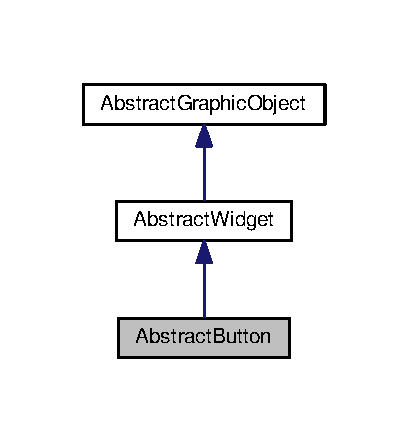
\includegraphics[width=196pt]{classAbstractButton__inherit__graph}
\end{center}
\end{figure}


Collaboration diagram for Abstract\+Button\+:
\nopagebreak
\begin{figure}[H]
\begin{center}
\leavevmode
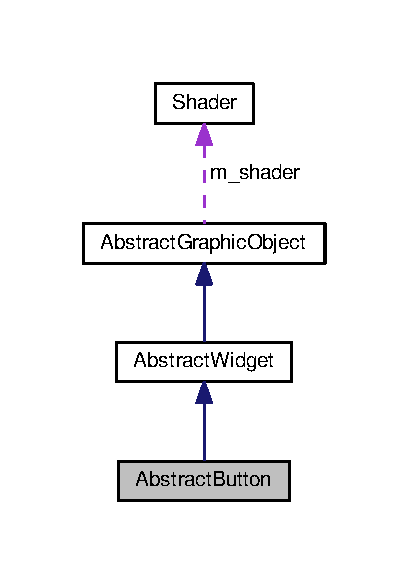
\includegraphics[width=196pt]{classAbstractButton__coll__graph}
\end{center}
\end{figure}
\subsection*{Public Member Functions}
\begin{DoxyCompactItemize}
\item 
\hypertarget{classAbstractButton_a1e6fec84d19280e39f0b4380b9de6029}{\hyperlink{classAbstractButton_a1e6fec84d19280e39f0b4380b9de6029}{Abstract\+Button} (\hyperlink{classShader}{Shader} $\ast$shad, glm\+::vec2 position, \hyperlink{classInput}{Input} $\ast$input)}\label{classAbstractButton_a1e6fec84d19280e39f0b4380b9de6029}

\begin{DoxyCompactList}\small\item\em Constructeur. \end{DoxyCompactList}\item 
\hypertarget{classAbstractButton_ae3d97004edc96ee5ccf9719df9c2458a}{\hyperlink{classAbstractButton_ae3d97004edc96ee5ccf9719df9c2458a}{$\sim$\+Abstract\+Button} ()}\label{classAbstractButton_ae3d97004edc96ee5ccf9719df9c2458a}

\begin{DoxyCompactList}\small\item\em Destructeur. \end{DoxyCompactList}\item 
\hypertarget{classAbstractButton_ad306c40d3966ae3d2187c88b426a1082}{virtual void \hyperlink{classAbstractButton_ad306c40d3966ae3d2187c88b426a1082}{draw} (glm\+::mat4 ortho)=0}\label{classAbstractButton_ad306c40d3966ae3d2187c88b426a1082}

\begin{DoxyCompactList}\small\item\em Méthode d'affichage (virtuelle pure) \end{DoxyCompactList}\item 
\hypertarget{classAbstractButton_a328cfee71f7ef2cced5b8b79e27f81e9}{void \hyperlink{classAbstractButton_a328cfee71f7ef2cced5b8b79e27f81e9}{set\+Dimensions} (glm\+::vec2 dim)}\label{classAbstractButton_a328cfee71f7ef2cced5b8b79e27f81e9}

\begin{DoxyCompactList}\small\item\em Modificateur de dimensions. \end{DoxyCompactList}\item 
\hypertarget{classAbstractButton_ab5e449bb4bd6a848c7dcd58b0644b0ec}{glm\+::vec2 \hyperlink{classAbstractButton_ab5e449bb4bd6a848c7dcd58b0644b0ec}{get\+Dimensions} () const }\label{classAbstractButton_ab5e449bb4bd6a848c7dcd58b0644b0ec}

\begin{DoxyCompactList}\small\item\em Retourne les dimensions. \end{DoxyCompactList}\end{DoxyCompactItemize}
\subsection*{Protected Member Functions}
\begin{DoxyCompactItemize}
\item 
\hypertarget{classAbstractButton_a15394cc151c318ea2bd66a53a978cfcb}{void \hyperlink{classAbstractButton_a15394cc151c318ea2bd66a53a978cfcb}{event\+Handler} ()}\label{classAbstractButton_a15394cc151c318ea2bd66a53a978cfcb}

\begin{DoxyCompactList}\small\item\em Gère les évênements. \end{DoxyCompactList}\item 
\hypertarget{classAbstractButton_a06155e27d4445be22b9444f21bc31567}{virtual void \hyperlink{classAbstractButton_a06155e27d4445be22b9444f21bc31567}{on\+Click\+Event} ()=0}\label{classAbstractButton_a06155e27d4445be22b9444f21bc31567}

\begin{DoxyCompactList}\small\item\em Virtuelle pure pour gérer le clic de souris. \end{DoxyCompactList}\end{DoxyCompactItemize}
\subsection*{Protected Attributes}
\begin{DoxyCompactItemize}
\item 
\hypertarget{classAbstractButton_a33c3fc97f6ef73e14100b5e509126b58}{bool \hyperlink{classAbstractButton_a33c3fc97f6ef73e14100b5e509126b58}{m\+\_\+stop\+Thread}}\label{classAbstractButton_a33c3fc97f6ef73e14100b5e509126b58}

\begin{DoxyCompactList}\small\item\em Booléen pour stopper les threads de gestion des évênements. \end{DoxyCompactList}\item 
\hypertarget{classAbstractButton_a178077a576ee755db7c839afea45bcc8}{std\+::thread \hyperlink{classAbstractButton_a178077a576ee755db7c839afea45bcc8}{m\+\_\+thread\+Click\+Event}}\label{classAbstractButton_a178077a576ee755db7c839afea45bcc8}

\begin{DoxyCompactList}\small\item\em Thread de gestion du clic de souris. \end{DoxyCompactList}\item 
\hypertarget{classAbstractButton_a949ebd940f2031815c706ff07f40a34c}{std\+::condition\+\_\+variable $\ast$ \hyperlink{classAbstractButton_a949ebd940f2031815c706ff07f40a34c}{m\+\_\+clicked}}\label{classAbstractButton_a949ebd940f2031815c706ff07f40a34c}

\begin{DoxyCompactList}\small\item\em Condition de gestion du clic de souris. \end{DoxyCompactList}\item 
\hypertarget{classAbstractButton_af964e22e2b6ee3fd0eb060dae764c425}{std\+::unique\+\_\+lock$<$ std\+::mutex $>$ \hyperlink{classAbstractButton_af964e22e2b6ee3fd0eb060dae764c425}{m\+\_\+clicked\+Lock}}\label{classAbstractButton_af964e22e2b6ee3fd0eb060dae764c425}

\begin{DoxyCompactList}\small\item\em Mutex de gestion du clic de souris. \end{DoxyCompactList}\item 
\hypertarget{classAbstractButton_aa2adf3970c7a506543514ca366c1be60}{glm\+::vec2 \hyperlink{classAbstractButton_aa2adf3970c7a506543514ca366c1be60}{m\+\_\+dimensions}}\label{classAbstractButton_aa2adf3970c7a506543514ca366c1be60}

\begin{DoxyCompactList}\small\item\em Dimensions du bouton. \end{DoxyCompactList}\end{DoxyCompactItemize}


\subsection{Detailed Description}
Type polymorphe pour les boutons. 

The documentation for this class was generated from the following files\+:\begin{DoxyCompactItemize}
\item 
\hyperlink{AbstractButton_8h}{Abstract\+Button.\+h}\item 
Abstract\+Button.\+cpp\end{DoxyCompactItemize}

\hypertarget{classAbstractCamera}{\section{Abstract\+Camera Class Reference}
\label{classAbstractCamera}\index{Abstract\+Camera@{Abstract\+Camera}}
}


Type polymorphe pour les caméras (point de vue sur le monde 3\+D)  




{\ttfamily \#include $<$Abstract\+Camera.\+h$>$}



Inheritance diagram for Abstract\+Camera\+:\nopagebreak
\begin{figure}[H]
\begin{center}
\leavevmode
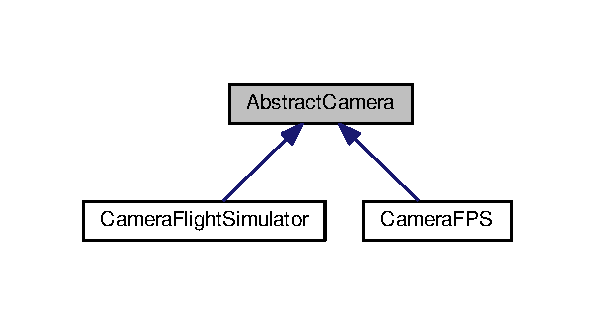
\includegraphics[width=286pt]{classAbstractCamera__inherit__graph}
\end{center}
\end{figure}
\subsection*{Public Member Functions}
\begin{DoxyCompactItemize}
\item 
\hypertarget{classAbstractCamera_a880ce099ca5cba2cb9baada64fb605b5}{\hyperlink{classAbstractCamera_a880ce099ca5cba2cb9baada64fb605b5}{Abstract\+Camera} (glm\+::vec3 const \&position, glm\+::vec3 const \&axe\+\_\+vertical, glm\+::vec3 const \&cible, float proche, float loin, float ratio\+Resolution)}\label{classAbstractCamera_a880ce099ca5cba2cb9baada64fb605b5}

\begin{DoxyCompactList}\small\item\em Construit une caméra et l'initialise en fonction de sa position de son axe vertical et de son point ciblé \end{DoxyCompactList}\item 
\hypertarget{classAbstractCamera_addf550f9f41d04bd6651b19d795bdabe}{virtual \hyperlink{classAbstractCamera_addf550f9f41d04bd6651b19d795bdabe}{$\sim$\+Abstract\+Camera} ()}\label{classAbstractCamera_addf550f9f41d04bd6651b19d795bdabe}

\begin{DoxyCompactList}\small\item\em Destructeur. \end{DoxyCompactList}\item 
\hypertarget{classAbstractCamera_a12f6c58003bece7aa6cb66108a1cbeb1}{virtual void \hyperlink{classAbstractCamera_a12f6c58003bece7aa6cb66108a1cbeb1}{look\+At} ()}\label{classAbstractCamera_a12f6c58003bece7aa6cb66108a1cbeb1}

\begin{DoxyCompactList}\small\item\em Méthode virtuelle qui doit construire et retourner la matrice de modelview. \end{DoxyCompactList}\item 
\hypertarget{classAbstractCamera_a7d34830e280d6c40ce3ff22583054880}{virtual void \hyperlink{classAbstractCamera_a7d34830e280d6c40ce3ff22583054880}{perspective} ()}\label{classAbstractCamera_a7d34830e280d6c40ce3ff22583054880}

\begin{DoxyCompactList}\small\item\em Méthode virtuelle pure qui doit construire et retourner la matrice de projection. \end{DoxyCompactList}\item 
\hypertarget{classAbstractCamera_a5dab83f71c638eda31fc49db01f47180}{virtual void \hyperlink{classAbstractCamera_a5dab83f71c638eda31fc49db01f47180}{on\+Event} (\hyperlink{classInput}{Input} const \&input)=0}\label{classAbstractCamera_a5dab83f71c638eda31fc49db01f47180}

\begin{DoxyCompactList}\small\item\em Méthode virtuelle pure qui traite les évênements pour la caméra appelée à chaque tour de boucle. \end{DoxyCompactList}\item 
\hypertarget{classAbstractCamera_a650255e1796dd50a2d95baa8c28fefae}{glm\+::mat4 \hyperlink{classAbstractCamera_a650255e1796dd50a2d95baa8c28fefae}{get\+Projection} () const }\label{classAbstractCamera_a650255e1796dd50a2d95baa8c28fefae}

\begin{DoxyCompactList}\small\item\em retourne la matrice de projection \end{DoxyCompactList}\item 
\hypertarget{classAbstractCamera_a31fa7a470de4ecd2437905ffd57cb40b}{glm\+::mat4 \hyperlink{classAbstractCamera_a31fa7a470de4ecd2437905ffd57cb40b}{get\+Modelview} () const }\label{classAbstractCamera_a31fa7a470de4ecd2437905ffd57cb40b}

\begin{DoxyCompactList}\small\item\em retourne la matrice de modelview \end{DoxyCompactList}\item 
\hypertarget{classAbstractCamera_ae6a61c6c50ffc278ad66f332e19e66a6}{virtual glm\+::vec3 \hyperlink{classAbstractCamera_ae6a61c6c50ffc278ad66f332e19e66a6}{get\+Position} () const =0}\label{classAbstractCamera_ae6a61c6c50ffc278ad66f332e19e66a6}

\begin{DoxyCompactList}\small\item\em Méthode virtuelle pure qui retourne la position. \end{DoxyCompactList}\item 
\hypertarget{classAbstractCamera_a1991c1773cda1eb142c9d127cf6e4107}{float \hyperlink{classAbstractCamera_a1991c1773cda1eb142c9d127cf6e4107}{get\+Vitesse} () const }\label{classAbstractCamera_a1991c1773cda1eb142c9d127cf6e4107}

\begin{DoxyCompactList}\small\item\em Retourne la vitesse. \end{DoxyCompactList}\item 
\hypertarget{classAbstractCamera_a625cd232811561751bd57493e2eadd20}{bool \hyperlink{classAbstractCamera_a625cd232811561751bd57493e2eadd20}{is\+Active} () const }\label{classAbstractCamera_a625cd232811561751bd57493e2eadd20}

\begin{DoxyCompactList}\small\item\em Savoir si la caméra est active(true) ou non(false) \end{DoxyCompactList}\item 
\hypertarget{classAbstractCamera_a0c7bbb7102072e5776646cb8ef04603f}{void \hyperlink{classAbstractCamera_a0c7bbb7102072e5776646cb8ef04603f}{set\+Active} (bool active)}\label{classAbstractCamera_a0c7bbb7102072e5776646cb8ef04603f}

\begin{DoxyCompactList}\small\item\em Déterminer si la caméra est active(true) ou non(false) \end{DoxyCompactList}\end{DoxyCompactItemize}
\subsection*{Protected Attributes}
\begin{DoxyCompactItemize}
\item 
\hypertarget{classAbstractCamera_a0a7cf1e2ab478c3b2a375fdd8d298cdc}{glm\+::vec3 \hyperlink{classAbstractCamera_a0a7cf1e2ab478c3b2a375fdd8d298cdc}{m\+\_\+position}}\label{classAbstractCamera_a0a7cf1e2ab478c3b2a375fdd8d298cdc}

\begin{DoxyCompactList}\small\item\em Position de la caméra dans le monde 3\+D. \end{DoxyCompactList}\item 
\hypertarget{classAbstractCamera_a9809fe9917c78f701bbda73a116b11cb}{glm\+::vec3 \hyperlink{classAbstractCamera_a9809fe9917c78f701bbda73a116b11cb}{m\+\_\+axe\+\_\+vertical}}\label{classAbstractCamera_a9809fe9917c78f701bbda73a116b11cb}

\begin{DoxyCompactList}\small\item\em Axe vertical de la caméra. \end{DoxyCompactList}\item 
\hypertarget{classAbstractCamera_aee9a00d7b11559a5448abbfa751a6d96}{glm\+::vec3 \hyperlink{classAbstractCamera_aee9a00d7b11559a5448abbfa751a6d96}{m\+\_\+cible}}\label{classAbstractCamera_aee9a00d7b11559a5448abbfa751a6d96}

\begin{DoxyCompactList}\small\item\em Point ciblé par la caméra. \end{DoxyCompactList}\item 
\hypertarget{classAbstractCamera_a16b6278ac154b9869c605131bab89d74}{glm\+::vec3 \hyperlink{classAbstractCamera_a16b6278ac154b9869c605131bab89d74}{m\+\_\+orientation}}\label{classAbstractCamera_a16b6278ac154b9869c605131bab89d74}

\begin{DoxyCompactList}\small\item\em Vecteur orientation de la caméra. \end{DoxyCompactList}\item 
\hypertarget{classAbstractCamera_a67b386323421b56e7e123d74c0d8e990}{glm\+::vec3 \hyperlink{classAbstractCamera_a67b386323421b56e7e123d74c0d8e990}{m\+\_\+droite}}\label{classAbstractCamera_a67b386323421b56e7e123d74c0d8e990}

\begin{DoxyCompactList}\small\item\em Vecteur normal à l'orientation et à l'axe vertical -\/$>$ deplacement lateral. \end{DoxyCompactList}\item 
\hypertarget{classAbstractCamera_a302613d43b644880473e964ede5c6094}{float \hyperlink{classAbstractCamera_a302613d43b644880473e964ede5c6094}{m\+\_\+proche}}\label{classAbstractCamera_a302613d43b644880473e964ede5c6094}

\begin{DoxyCompactList}\small\item\em Distance minimale de la caméra pour affichage. \end{DoxyCompactList}\item 
\hypertarget{classAbstractCamera_a29c540279b97ed810fdd7afd65bf6b4e}{float \hyperlink{classAbstractCamera_a29c540279b97ed810fdd7afd65bf6b4e}{m\+\_\+loin}}\label{classAbstractCamera_a29c540279b97ed810fdd7afd65bf6b4e}

\begin{DoxyCompactList}\small\item\em Distance maximale de la caméra pour affichage. \end{DoxyCompactList}\item 
\hypertarget{classAbstractCamera_ac4dccb042e77bb91c2aa66a315112043}{float \hyperlink{classAbstractCamera_ac4dccb042e77bb91c2aa66a315112043}{m\+\_\+ratio\+Resolution}}\label{classAbstractCamera_ac4dccb042e77bb91c2aa66a315112043}

\begin{DoxyCompactList}\small\item\em Largeur de la fenêtre / Hauteur de la fenêtre. \end{DoxyCompactList}\item 
\hypertarget{classAbstractCamera_a554f06bd5f27d68700f844cc4e6b7dba}{float \hyperlink{classAbstractCamera_a554f06bd5f27d68700f844cc4e6b7dba}{m\+\_\+vitesse}}\label{classAbstractCamera_a554f06bd5f27d68700f844cc4e6b7dba}

\begin{DoxyCompactList}\small\item\em Vitesse de déplacement de la caméra. \end{DoxyCompactList}\item 
\hypertarget{classAbstractCamera_aa99260e08a54ece7bcfc81ca44baf82c}{glm\+::mat4 \hyperlink{classAbstractCamera_aa99260e08a54ece7bcfc81ca44baf82c}{m\+\_\+projection}}\label{classAbstractCamera_aa99260e08a54ece7bcfc81ca44baf82c}

\begin{DoxyCompactList}\small\item\em Matrice de projection. \end{DoxyCompactList}\item 
\hypertarget{classAbstractCamera_aa26d2fe7b5921b46c5721e17e3a05c15}{glm\+::mat4 \hyperlink{classAbstractCamera_aa26d2fe7b5921b46c5721e17e3a05c15}{m\+\_\+modelview}}\label{classAbstractCamera_aa26d2fe7b5921b46c5721e17e3a05c15}

\begin{DoxyCompactList}\small\item\em Matrice de modelview. \end{DoxyCompactList}\item 
\hypertarget{classAbstractCamera_ad40646721bbb5ec24fe9fb2080763e51}{bool \hyperlink{classAbstractCamera_ad40646721bbb5ec24fe9fb2080763e51}{m\+\_\+active}}\label{classAbstractCamera_ad40646721bbb5ec24fe9fb2080763e51}

\begin{DoxyCompactList}\small\item\em Détermine si la caméra est active ou non. \end{DoxyCompactList}\end{DoxyCompactItemize}


\subsection{Detailed Description}
Type polymorphe pour les caméras (point de vue sur le monde 3\+D) 

The documentation for this class was generated from the following file\+:\begin{DoxyCompactItemize}
\item 
\hyperlink{AbstractCamera_8h}{Abstract\+Camera.\+h}\end{DoxyCompactItemize}

\hypertarget{classAbstractGraphicObject}{\section{Abstract\+Graphic\+Object Class Reference}
\label{classAbstractGraphicObject}\index{Abstract\+Graphic\+Object@{Abstract\+Graphic\+Object}}
}


Classe abstraite définissant un type polymorphe pour les objets graphiques.  




{\ttfamily \#include $<$Abstract\+Graphic\+Object.\+h$>$}



Inheritance diagram for Abstract\+Graphic\+Object\+:
\nopagebreak
\begin{figure}[H]
\begin{center}
\leavevmode
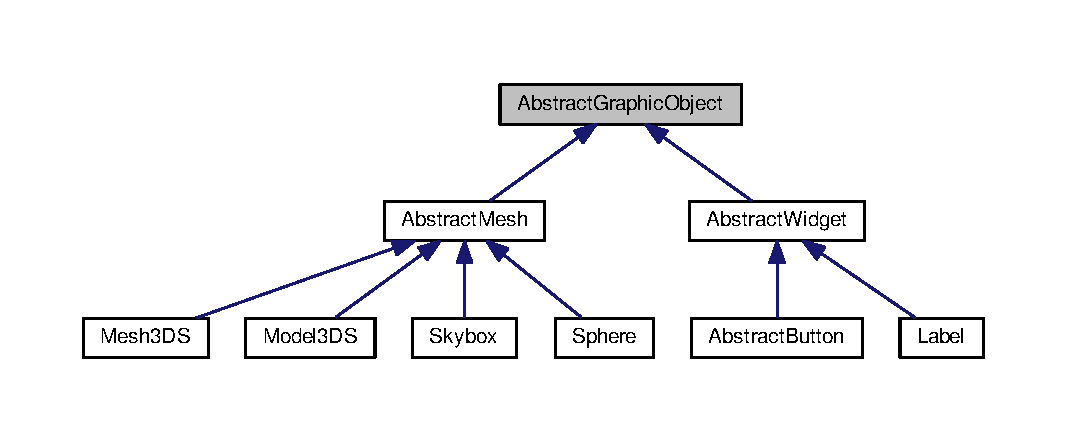
\includegraphics[width=350pt]{classAbstractGraphicObject__inherit__graph}
\end{center}
\end{figure}


Collaboration diagram for Abstract\+Graphic\+Object\+:\nopagebreak
\begin{figure}[H]
\begin{center}
\leavevmode
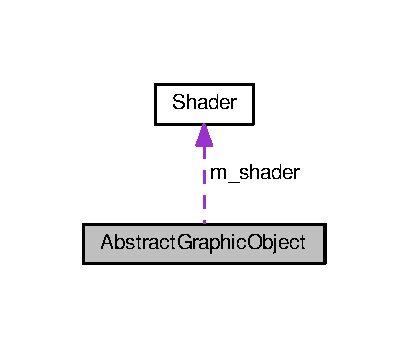
\includegraphics[width=196pt]{classAbstractGraphicObject__coll__graph}
\end{center}
\end{figure}
\subsection*{Public Member Functions}
\begin{DoxyCompactItemize}
\item 
\hypertarget{classAbstractGraphicObject_ab1ddb96b82b01bba5e56e0917dceba0c}{\hyperlink{classAbstractGraphicObject_ab1ddb96b82b01bba5e56e0917dceba0c}{Abstract\+Graphic\+Object} (\hyperlink{classShader}{Shader} $\ast$shad)}\label{classAbstractGraphicObject_ab1ddb96b82b01bba5e56e0917dceba0c}

\begin{DoxyCompactList}\small\item\em Construit un objet graphique en utilisant le shader donné en argument pour le rendu. \end{DoxyCompactList}\item 
\hypertarget{classAbstractGraphicObject_aa20078bf878fc72814a44d5a986ec548}{virtual \hyperlink{classAbstractGraphicObject_aa20078bf878fc72814a44d5a986ec548}{$\sim$\+Abstract\+Graphic\+Object} ()}\label{classAbstractGraphicObject_aa20078bf878fc72814a44d5a986ec548}

\begin{DoxyCompactList}\small\item\em Destructeur. \end{DoxyCompactList}\item 
\hypertarget{classAbstractGraphicObject_ae0e201a972ea7e97b032bf21f75390a7}{virtual void \hyperlink{classAbstractGraphicObject_ae0e201a972ea7e97b032bf21f75390a7}{load} ()=0}\label{classAbstractGraphicObject_ae0e201a972ea7e97b032bf21f75390a7}

\begin{DoxyCompactList}\small\item\em Génère les objets opengl (vbo,vao,textures) pour cet objet graphique. \end{DoxyCompactList}\item 
\hypertarget{classAbstractGraphicObject_a69f33de948f6a754f6c345e5ad439e89}{virtual void \hyperlink{classAbstractGraphicObject_a69f33de948f6a754f6c345e5ad439e89}{clean\+Up} ()}\label{classAbstractGraphicObject_a69f33de948f6a754f6c345e5ad439e89}

\begin{DoxyCompactList}\small\item\em Détruit les objets de construction intermédiaires. \end{DoxyCompactList}\end{DoxyCompactItemize}
\subsection*{Protected Attributes}
\begin{DoxyCompactItemize}
\item 
\hypertarget{classAbstractGraphicObject_a7e1566fbd2b769d12dc43ed9a4dd61f1}{G\+Luint \hyperlink{classAbstractGraphicObject_a7e1566fbd2b769d12dc43ed9a4dd61f1}{m\+\_\+vbo\+I\+D}}\label{classAbstractGraphicObject_a7e1566fbd2b769d12dc43ed9a4dd61f1}

\begin{DoxyCompactList}\small\item\em Identifiant Open\+G\+L du Vertex Buffer Object (V\+B\+O) (généré lors de l'appel de \hyperlink{classAbstractGraphicObject_ae0e201a972ea7e97b032bf21f75390a7}{load()}) \end{DoxyCompactList}\item 
\hypertarget{classAbstractGraphicObject_aa0fd0c978efb2e99ef3393afcb779313}{G\+Luint \hyperlink{classAbstractGraphicObject_aa0fd0c978efb2e99ef3393afcb779313}{m\+\_\+vao\+I\+D}}\label{classAbstractGraphicObject_aa0fd0c978efb2e99ef3393afcb779313}

\begin{DoxyCompactList}\small\item\em Identifiant Open\+G\+L du Vertex Array Object (V\+A\+O) (généré lors de l'appel de \hyperlink{classAbstractGraphicObject_ae0e201a972ea7e97b032bf21f75390a7}{load()}) \end{DoxyCompactList}\item 
\hypertarget{classAbstractGraphicObject_a75da74184185de4e01d232a92a2d2b68}{\hyperlink{classShader}{Shader} $\ast$ \hyperlink{classAbstractGraphicObject_a75da74184185de4e01d232a92a2d2b68}{m\+\_\+shader}}\label{classAbstractGraphicObject_a75da74184185de4e01d232a92a2d2b68}

\begin{DoxyCompactList}\small\item\em \hyperlink{classShader}{Shader} pour le rendu (les shaders sont gérés en externe par les classes \hyperlink{classGuiFactory}{Gui\+Factory} -\/$>$ 2\+D ou Scene\+Factory -\/$>$ 3\+D ) \end{DoxyCompactList}\item 
\hypertarget{classAbstractGraphicObject_a302995e5cd2cc5565fbe631194e967e1}{std\+::vector$<$ float $>$ \hyperlink{classAbstractGraphicObject_a302995e5cd2cc5565fbe631194e967e1}{m\+\_\+vertices}}\label{classAbstractGraphicObject_a302995e5cd2cc5565fbe631194e967e1}

\begin{DoxyCompactList}\small\item\em Tableau temporaire de sommets. \end{DoxyCompactList}\end{DoxyCompactItemize}


\subsection{Detailed Description}
Classe abstraite définissant un type polymorphe pour les objets graphiques. 

The documentation for this class was generated from the following file\+:\begin{DoxyCompactItemize}
\item 
\hyperlink{AbstractGraphicObject_8h}{Abstract\+Graphic\+Object.\+h}\end{DoxyCompactItemize}

\hypertarget{classAbstractMesh}{\section{Abstract\+Mesh Class Reference}
\label{classAbstractMesh}\index{Abstract\+Mesh@{Abstract\+Mesh}}
}


Type polymorphe pour les modèles 3\+D.  




{\ttfamily \#include $<$Abstract\+Mesh.\+h$>$}



Inheritance diagram for Abstract\+Mesh\+:\nopagebreak
\begin{figure}[H]
\begin{center}
\leavevmode
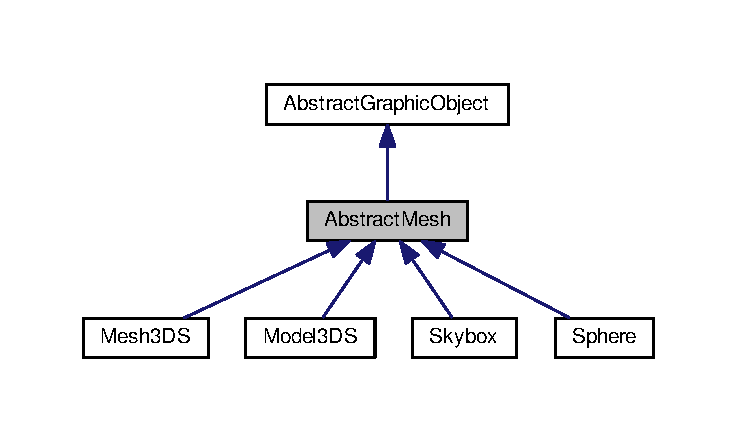
\includegraphics[width=350pt]{classAbstractMesh__inherit__graph}
\end{center}
\end{figure}


Collaboration diagram for Abstract\+Mesh\+:\nopagebreak
\begin{figure}[H]
\begin{center}
\leavevmode
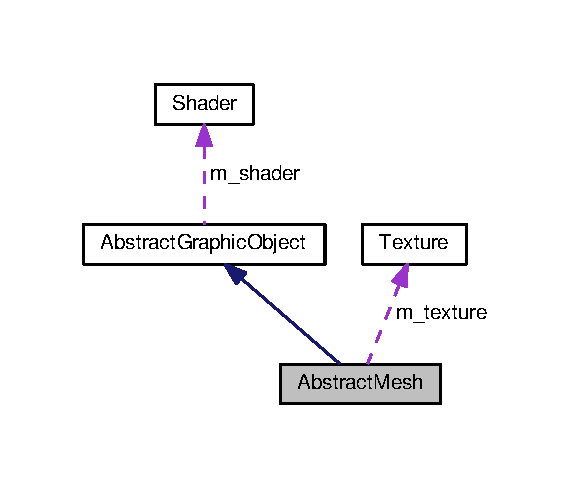
\includegraphics[width=274pt]{classAbstractMesh__coll__graph}
\end{center}
\end{figure}
\subsection*{Public Member Functions}
\begin{DoxyCompactItemize}
\item 
\hypertarget{classAbstractMesh_ade7bd3d65928c4676be31263bafc8a71}{\hyperlink{classAbstractMesh_ade7bd3d65928c4676be31263bafc8a71}{Abstract\+Mesh} (\hyperlink{classShader}{Shader} $\ast$shader, \hyperlink{classTexture}{Texture} $\ast$texture)}\label{classAbstractMesh_ade7bd3d65928c4676be31263bafc8a71}

\begin{DoxyCompactList}\small\item\em Constructeur à partir de la texture donnés en argument. \end{DoxyCompactList}\item 
\hypertarget{classAbstractMesh_a6a2a3bd0e2e321707ec7fef7ff933ba6}{\hyperlink{classAbstractMesh_a6a2a3bd0e2e321707ec7fef7ff933ba6}{Abstract\+Mesh} (\hyperlink{classAbstractMesh}{Abstract\+Mesh} $\ast$mesh)}\label{classAbstractMesh_a6a2a3bd0e2e321707ec7fef7ff933ba6}

\begin{DoxyCompactList}\small\item\em Constructeur de copie. \end{DoxyCompactList}\item 
\hypertarget{classAbstractMesh_a9688f69d4431eb08c7b65693d0fffd9e}{virtual void \hyperlink{classAbstractMesh_a9688f69d4431eb08c7b65693d0fffd9e}{load} ()}\label{classAbstractMesh_a9688f69d4431eb08c7b65693d0fffd9e}

\begin{DoxyCompactList}\small\item\em Construit les objets Open\+G\+L (vbo et vao) pour ce modèle. \end{DoxyCompactList}\item 
\hypertarget{classAbstractMesh_aef065877afe59562920748e265196c82}{virtual void \hyperlink{classAbstractMesh_aef065877afe59562920748e265196c82}{draw} (glm\+::mat4 mvp)=0}\label{classAbstractMesh_aef065877afe59562920748e265196c82}

\begin{DoxyCompactList}\small\item\em Méthode virtuelle pure qui affiche le mesh en fonction de la matrice de modelview\+Projection. \end{DoxyCompactList}\item 
\hypertarget{classAbstractMesh_a996ae58b3352c31f834a07ab0b071d6c}{virtual void \hyperlink{classAbstractMesh_a996ae58b3352c31f834a07ab0b071d6c}{clean\+Up} ()}\label{classAbstractMesh_a996ae58b3352c31f834a07ab0b071d6c}

\begin{DoxyCompactList}\small\item\em Détruit les objets de construction intermédiaires. \end{DoxyCompactList}\end{DoxyCompactItemize}
\subsection*{Protected Attributes}
\begin{DoxyCompactItemize}
\item 
\hypertarget{classAbstractMesh_a15e43124d601085e1495c738a657c826}{std\+::vector$<$ float $>$ \hyperlink{classAbstractMesh_a15e43124d601085e1495c738a657c826}{m\+\_\+coord\+Tex}}\label{classAbstractMesh_a15e43124d601085e1495c738a657c826}

\begin{DoxyCompactList}\small\item\em Tableau de coordonnées de textures. \end{DoxyCompactList}\item 
\hypertarget{classAbstractMesh_a0bcd16f81880e90b11781bb61af294cf}{\hyperlink{classTexture}{Texture} $\ast$ \hyperlink{classAbstractMesh_a0bcd16f81880e90b11781bb61af294cf}{m\+\_\+texture}}\label{classAbstractMesh_a0bcd16f81880e90b11781bb61af294cf}

\begin{DoxyCompactList}\small\item\em \hyperlink{classTexture}{Texture} de l'objet. \end{DoxyCompactList}\item 
\hypertarget{classAbstractMesh_a07951f17a49c5a02a895ca6cbdd3b0c5}{unsigned long \hyperlink{classAbstractMesh_a07951f17a49c5a02a895ca6cbdd3b0c5}{m\+\_\+nb\+Vertices}}\label{classAbstractMesh_a07951f17a49c5a02a895ca6cbdd3b0c5}

\begin{DoxyCompactList}\small\item\em Nombre de vertices de ce mesh. \end{DoxyCompactList}\end{DoxyCompactItemize}


\subsection{Detailed Description}
Type polymorphe pour les modèles 3\+D. 

The documentation for this class was generated from the following files\+:\begin{DoxyCompactItemize}
\item 
\hyperlink{AbstractMesh_8h}{Abstract\+Mesh.\+h}\item 
Abstract\+Mesh.\+cpp\end{DoxyCompactItemize}

\hypertarget{classAbstractWidget}{\section{Abstract\+Widget Class Reference}
\label{classAbstractWidget}\index{Abstract\+Widget@{Abstract\+Widget}}
}


Classe abstraite mère de tous les objets 2\+D.  




{\ttfamily \#include $<$Abstract\+Widget.\+h$>$}



Inheritance diagram for Abstract\+Widget\+:
\nopagebreak
\begin{figure}[H]
\begin{center}
\leavevmode
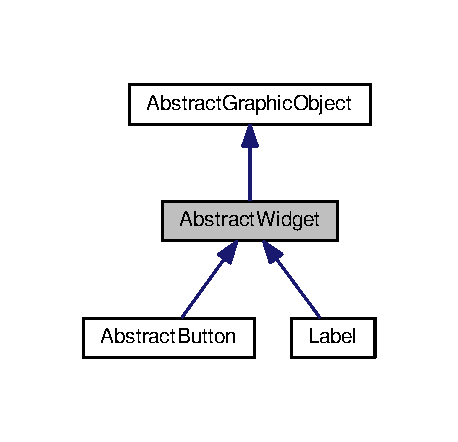
\includegraphics[width=220pt]{classAbstractWidget__inherit__graph}
\end{center}
\end{figure}


Collaboration diagram for Abstract\+Widget\+:\nopagebreak
\begin{figure}[H]
\begin{center}
\leavevmode
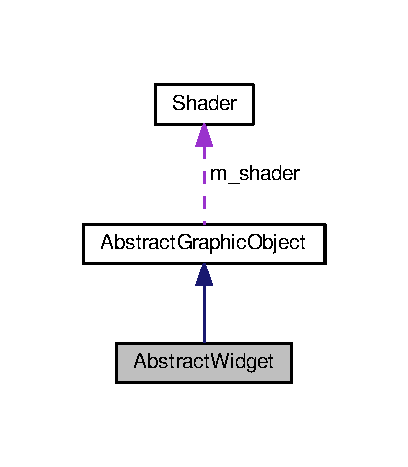
\includegraphics[width=196pt]{classAbstractWidget__coll__graph}
\end{center}
\end{figure}
\subsection*{Public Member Functions}
\begin{DoxyCompactItemize}
\item 
\hypertarget{classAbstractWidget_a385f0b11064be82084e3141602a2962e}{\hyperlink{classAbstractWidget_a385f0b11064be82084e3141602a2962e}{Abstract\+Widget} (\hyperlink{classShader}{Shader} $\ast$shader, glm\+::vec2 position)}\label{classAbstractWidget_a385f0b11064be82084e3141602a2962e}

\begin{DoxyCompactList}\small\item\em Crée un objet 2\+D à la position sur l'écran indiquée en argument. \end{DoxyCompactList}\item 
\hypertarget{classAbstractWidget_ace1ce0f76aeb82b810a0ac50059a0e59}{virtual \hyperlink{classAbstractWidget_ace1ce0f76aeb82b810a0ac50059a0e59}{$\sim$\+Abstract\+Widget} ()}\label{classAbstractWidget_ace1ce0f76aeb82b810a0ac50059a0e59}

\begin{DoxyCompactList}\small\item\em Détruit un objet2\+D et libère ses ressources. \end{DoxyCompactList}\item 
\hypertarget{classAbstractWidget_a1ad11e1303e1f73f77726a24167f943f}{glm\+::vec2 \hyperlink{classAbstractWidget_a1ad11e1303e1f73f77726a24167f943f}{get\+Position} ()}\label{classAbstractWidget_a1ad11e1303e1f73f77726a24167f943f}

\begin{DoxyCompactList}\small\item\em Retourne la position d l'objet sur l'écran. \end{DoxyCompactList}\item 
\hypertarget{classAbstractWidget_acc96658ec6504098e7e9cadcc78c3197}{void \hyperlink{classAbstractWidget_acc96658ec6504098e7e9cadcc78c3197}{set\+Position} (glm\+::vec2 const \&position)}\label{classAbstractWidget_acc96658ec6504098e7e9cadcc78c3197}

\begin{DoxyCompactList}\small\item\em Change la position d'un objet 2\+D sur l'écran. \end{DoxyCompactList}\item 
\hypertarget{classAbstractWidget_aa4fcf0bffd64956bda11ee5302641def}{virtual void \hyperlink{classAbstractWidget_aa4fcf0bffd64956bda11ee5302641def}{draw} (glm\+::mat4 ortho)=0}\label{classAbstractWidget_aa4fcf0bffd64956bda11ee5302641def}

\begin{DoxyCompactList}\small\item\em Méthode virtuelle pure d'affichage) \end{DoxyCompactList}\end{DoxyCompactItemize}
\subsection*{Protected Attributes}
\begin{DoxyCompactItemize}
\item 
\hypertarget{classAbstractWidget_a847822efcb2b75b9696e1fc9b4ecfa88}{glm\+::vec2 \hyperlink{classAbstractWidget_a847822efcb2b75b9696e1fc9b4ecfa88}{m\+\_\+position}}\label{classAbstractWidget_a847822efcb2b75b9696e1fc9b4ecfa88}

\begin{DoxyCompactList}\small\item\em Position de l'objet sur l'écran. \end{DoxyCompactList}\end{DoxyCompactItemize}


\subsection{Detailed Description}
Classe abstraite mère de tous les objets 2\+D. 

The documentation for this class was generated from the following file\+:\begin{DoxyCompactItemize}
\item 
\hyperlink{AbstractWidget_8h}{Abstract\+Widget.\+h}\end{DoxyCompactItemize}

\hypertarget{classApplicationControl}{\section{Application\+Control Class Reference}
\label{classApplicationControl}\index{Application\+Control@{Application\+Control}}
}


Classe repésentant globalement le programme graphique.  




{\ttfamily \#include $<$Application\+Control.\+h$>$}

\subsection*{Public Member Functions}
\begin{DoxyCompactItemize}
\item 
\hypertarget{classApplicationControl_a0297dd9aebc1dec0b82ec9b52ef834ad}{\hyperlink{classApplicationControl_a0297dd9aebc1dec0b82ec9b52ef834ad}{Application\+Control} (unsigned int window\+Width=800, unsigned int window\+Height=600)}\label{classApplicationControl_a0297dd9aebc1dec0b82ec9b52ef834ad}

\begin{DoxyCompactList}\small\item\em Crée la fenetre à l'aide des dimensions en argument. \end{DoxyCompactList}\item 
\hypertarget{classApplicationControl_a77142ab2e6afa9bc4b470a00b41aed77}{\hyperlink{classApplicationControl_a77142ab2e6afa9bc4b470a00b41aed77}{$\sim$\+Application\+Control} ()}\label{classApplicationControl_a77142ab2e6afa9bc4b470a00b41aed77}

\begin{DoxyCompactList}\small\item\em Destructeur. \end{DoxyCompactList}\item 
\hypertarget{classApplicationControl_a11c3f05fcf4c19e4be15ef49cec06a43}{bool \hyperlink{classApplicationControl_a11c3f05fcf4c19e4be15ef49cec06a43}{init} ()}\label{classApplicationControl_a11c3f05fcf4c19e4be15ef49cec06a43}

\begin{DoxyCompactList}\small\item\em initialisation de la S\+D\+L, de Open\+G\+L ainsi que de la fenêtre \end{DoxyCompactList}\item 
\hypertarget{classApplicationControl_ae2fa75e6d29ef2479d47076f1a780113}{bool \hyperlink{classApplicationControl_ae2fa75e6d29ef2479d47076f1a780113}{execute} ()}\label{classApplicationControl_ae2fa75e6d29ef2479d47076f1a780113}

\begin{DoxyCompactList}\small\item\em Exécution du programme graphique. \end{DoxyCompactList}\end{DoxyCompactItemize}


\subsection{Detailed Description}
Classe repésentant globalement le programme graphique. 

The documentation for this class was generated from the following files\+:\begin{DoxyCompactItemize}
\item 
\hyperlink{ApplicationControl_8h}{Application\+Control.\+h}\item 
Application\+Control.\+cpp\end{DoxyCompactItemize}

\hypertarget{classCameraFlightSimulator}{\section{Camera\-Flight\-Simulator Class Reference}
\label{classCameraFlightSimulator}\index{Camera\-Flight\-Simulator@{Camera\-Flight\-Simulator}}
}


Implémentation de la caméra de simulateur de vol.  




{\ttfamily \#include $<$Camera\-Flight\-Simulator.\-h$>$}

Inheritance diagram for Camera\-Flight\-Simulator\-:\begin{figure}[H]
\begin{center}
\leavevmode
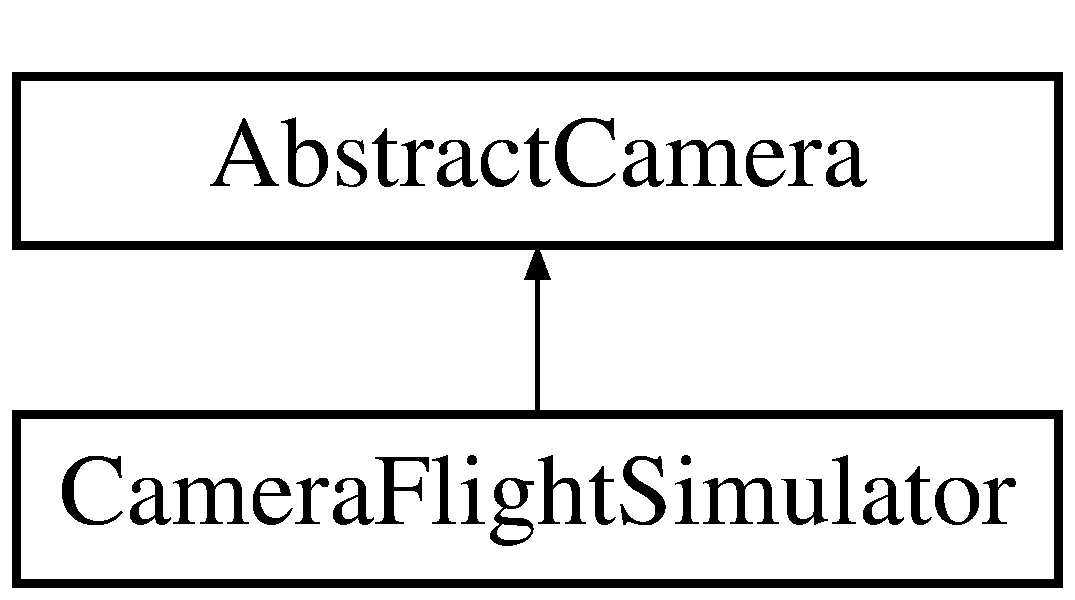
\includegraphics[height=2.000000cm]{classCameraFlightSimulator}
\end{center}
\end{figure}
\subsection*{Public Member Functions}
\begin{DoxyCompactItemize}
\item 
\hypertarget{classCameraFlightSimulator_a13b192b01617281f3dcf9b7acb8e0d44}{\hyperlink{classCameraFlightSimulator_a13b192b01617281f3dcf9b7acb8e0d44}{Camera\-Flight\-Simulator} (glm\-::vec3 const \&position, glm\-::vec3 const \&axe\-\_\-vertical, glm\-::vec3 const \&cible, float proche, float loin, float ratio\-Resolution, \hyperlink{classMeshNode}{Mesh\-Node} $\ast$attached)}\label{classCameraFlightSimulator_a13b192b01617281f3dcf9b7acb8e0d44}

\begin{DoxyCompactList}\small\item\em Constructeur de caméra de simulateur de vol. \end{DoxyCompactList}\item 
\hypertarget{classCameraFlightSimulator_aa83f01c1f64fd6fbf56c341866cb62f8}{virtual \hyperlink{classCameraFlightSimulator_aa83f01c1f64fd6fbf56c341866cb62f8}{$\sim$\-Camera\-Flight\-Simulator} ()}\label{classCameraFlightSimulator_aa83f01c1f64fd6fbf56c341866cb62f8}

\begin{DoxyCompactList}\small\item\em Destructeur. \end{DoxyCompactList}\item 
\hypertarget{classCameraFlightSimulator_ae8ea1ed382e1dfdde4f53ad654c503f5}{virtual void \hyperlink{classCameraFlightSimulator_ae8ea1ed382e1dfdde4f53ad654c503f5}{on\-Event} (\hyperlink{classInput}{Input} const \&input)}\label{classCameraFlightSimulator_ae8ea1ed382e1dfdde4f53ad654c503f5}

\begin{DoxyCompactList}\small\item\em Traitement des évênements clavier. \end{DoxyCompactList}\item 
\hypertarget{classCameraFlightSimulator_ab624dcd6b9110c82980ec2d04786da6d}{virtual glm\-::vec3 \hyperlink{classCameraFlightSimulator_ab624dcd6b9110c82980ec2d04786da6d}{get\-Position} () const }\label{classCameraFlightSimulator_ab624dcd6b9110c82980ec2d04786da6d}

\begin{DoxyCompactList}\small\item\em Méthode virtuelle qui retourne la position. \end{DoxyCompactList}\item 
\hypertarget{classCameraFlightSimulator_a70d900c0f14c3193b9af612ad8f48249}{virtual void \hyperlink{classCameraFlightSimulator_a70d900c0f14c3193b9af612ad8f48249}{perspective} ()}\label{classCameraFlightSimulator_a70d900c0f14c3193b9af612ad8f48249}

\begin{DoxyCompactList}\small\item\em Méthode virtuelle pure qui doit construire et retourner la matrice de projection. \end{DoxyCompactList}\end{DoxyCompactItemize}
\subsection*{Additional Inherited Members}


\subsection{Detailed Description}
Implémentation de la caméra de simulateur de vol. 

The documentation for this class was generated from the following files\-:\begin{DoxyCompactItemize}
\item 
\hyperlink{CameraFlightSimulator_8h}{Camera\-Flight\-Simulator.\-h}\item 
Camera\-Flight\-Simulator.\-cpp\end{DoxyCompactItemize}

\hypertarget{classCameraFPS}{\section{Camera\-F\-P\-S Class Reference}
\label{classCameraFPS}\index{Camera\-F\-P\-S@{Camera\-F\-P\-S}}
}


Caméra de type Freefly à deux degrés de liberté en fixant l'axe vertical.  




{\ttfamily \#include $<$Camera\-F\-P\-S.\-h$>$}

Inheritance diagram for Camera\-F\-P\-S\-:\begin{figure}[H]
\begin{center}
\leavevmode
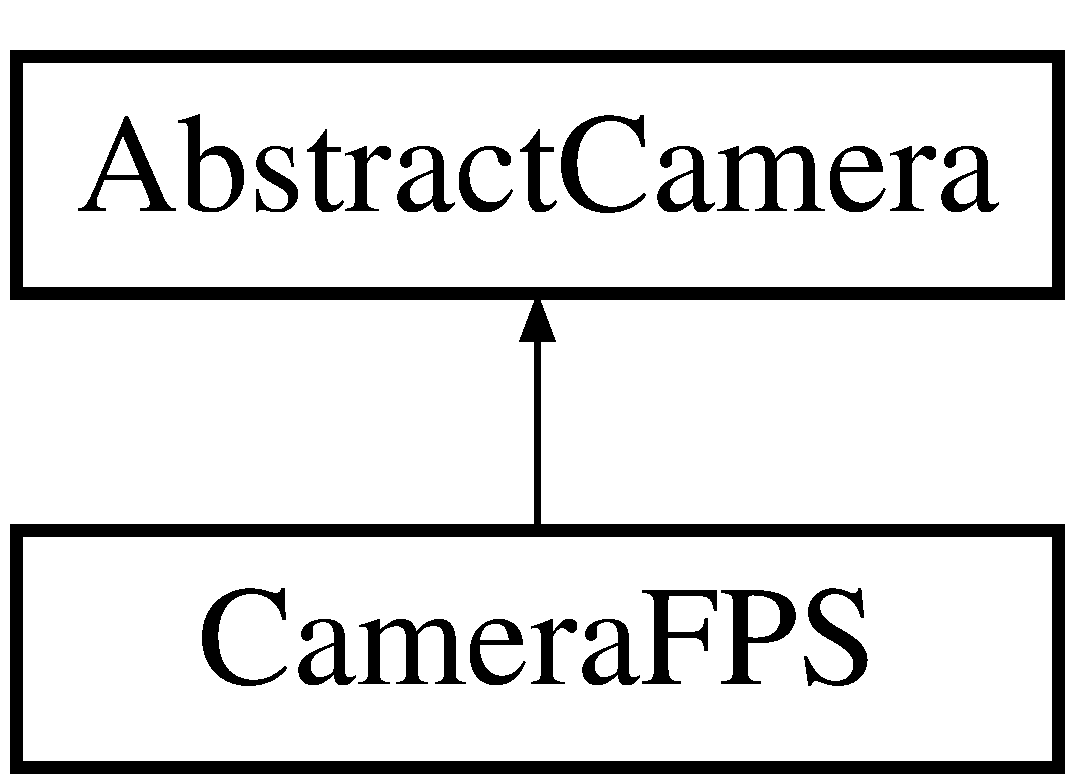
\includegraphics[height=2.000000cm]{classCameraFPS}
\end{center}
\end{figure}
\subsection*{Public Member Functions}
\begin{DoxyCompactItemize}
\item 
\hypertarget{classCameraFPS_a052e711986b70b0f34fb85f72c6818c9}{\hyperlink{classCameraFPS_a052e711986b70b0f34fb85f72c6818c9}{Camera\-F\-P\-S} (glm\-::vec3 const \&position, glm\-::vec3 const \&axe\-\_\-vertical, glm\-::vec3 const \&cible, float proche, float loin, float ratio\-Resolution, float vitesse, float sensibilite)}\label{classCameraFPS_a052e711986b70b0f34fb85f72c6818c9}

\begin{DoxyCompactList}\small\item\em Création et initialisation. \end{DoxyCompactList}\item 
\hypertarget{classCameraFPS_a2cf832c958d3e5a630539ea864b484dd}{\hyperlink{classCameraFPS_a2cf832c958d3e5a630539ea864b484dd}{$\sim$\-Camera\-F\-P\-S} ()}\label{classCameraFPS_a2cf832c958d3e5a630539ea864b484dd}

\begin{DoxyCompactList}\small\item\em Destructeur. \end{DoxyCompactList}\item 
\hypertarget{classCameraFPS_a1a051bc9f334ec12dc43fa16f6dd204c}{virtual void \hyperlink{classCameraFPS_a1a051bc9f334ec12dc43fa16f6dd204c}{on\-Event} (\hyperlink{classInput}{Input} const \&input)}\label{classCameraFPS_a1a051bc9f334ec12dc43fa16f6dd204c}

\begin{DoxyCompactList}\small\item\em Traitement des évênements clavier et souris. \end{DoxyCompactList}\item 
\hypertarget{classCameraFPS_a09b8ff24683ec75c107fce3e502eea1f}{virtual void \hyperlink{classCameraFPS_a09b8ff24683ec75c107fce3e502eea1f}{perspective} ()}\label{classCameraFPS_a09b8ff24683ec75c107fce3e502eea1f}

\begin{DoxyCompactList}\small\item\em Méthode virtuelle qui doit construire et retourner la matrice de projection pour prendre en compte le zoom. \end{DoxyCompactList}\item 
\hypertarget{classCameraFPS_a46be704d8fc6c8c25f9e6d093916affb}{virtual glm\-::vec3 \hyperlink{classCameraFPS_a46be704d8fc6c8c25f9e6d093916affb}{get\-Position} () const }\label{classCameraFPS_a46be704d8fc6c8c25f9e6d093916affb}

\begin{DoxyCompactList}\small\item\em retourne la position \end{DoxyCompactList}\end{DoxyCompactItemize}
\subsection*{Protected Member Functions}
\begin{DoxyCompactItemize}
\item 
\hypertarget{classCameraFPS_a0b06955072fe29f6cf8a5c76828025fd}{void \hyperlink{classCameraFPS_a0b06955072fe29f6cf8a5c76828025fd}{orienter} (int x\-Rel, int y\-Rel)}\label{classCameraFPS_a0b06955072fe29f6cf8a5c76828025fd}

\begin{DoxyCompactList}\small\item\em Oriente la caméra en fonction du déplacement de la souris. \end{DoxyCompactList}\item 
\hypertarget{classCameraFPS_af71850751b121f12f25b03f75e836cc5}{void \hyperlink{classCameraFPS_af71850751b121f12f25b03f75e836cc5}{deplacer} (glm\-::vec3 const \&deplacement)}\label{classCameraFPS_af71850751b121f12f25b03f75e836cc5}

\begin{DoxyCompactList}\small\item\em Déplace la caméra. \end{DoxyCompactList}\item 
\hypertarget{classCameraFPS_a073a8db2ee3711140d0b0fc1a36086cd}{void \hyperlink{classCameraFPS_a073a8db2ee3711140d0b0fc1a36086cd}{zoomer} (int zoom)}\label{classCameraFPS_a073a8db2ee3711140d0b0fc1a36086cd}

\begin{DoxyCompactList}\small\item\em Effectue un zoome dans le monde 3\-D. \end{DoxyCompactList}\end{DoxyCompactItemize}
\subsection*{Protected Attributes}
\begin{DoxyCompactItemize}
\item 
\hypertarget{classCameraFPS_adea819c2cc3cbe4d12153e18a61eef4d}{float \hyperlink{classCameraFPS_adea819c2cc3cbe4d12153e18a61eef4d}{m\-\_\-phi}}\label{classCameraFPS_adea819c2cc3cbe4d12153e18a61eef4d}

\begin{DoxyCompactList}\small\item\em Angle de rotation par rapport à l'axe vertical. \end{DoxyCompactList}\item 
\hypertarget{classCameraFPS_a9980f2a325bf21f2bbadf3d3caceebc5}{float \hyperlink{classCameraFPS_a9980f2a325bf21f2bbadf3d3caceebc5}{m\-\_\-theta}}\label{classCameraFPS_a9980f2a325bf21f2bbadf3d3caceebc5}

\begin{DoxyCompactList}\small\item\em Angle de rotation par rapport au vecteur lateral. \end{DoxyCompactList}\item 
\hypertarget{classCameraFPS_af473984bd2b269434960ec381b59682c}{float \hyperlink{classCameraFPS_af473984bd2b269434960ec381b59682c}{m\-\_\-zoom}}\label{classCameraFPS_af473984bd2b269434960ec381b59682c}

\begin{DoxyCompactList}\small\item\em Zoom de la caméra. \end{DoxyCompactList}\item 
\hypertarget{classCameraFPS_acf2f083c8757a1571165f4e8b6d3feba}{float \hyperlink{classCameraFPS_acf2f083c8757a1571165f4e8b6d3feba}{m\-\_\-sensibilite}}\label{classCameraFPS_acf2f083c8757a1571165f4e8b6d3feba}

\begin{DoxyCompactList}\small\item\em Vitesse de rotation de la caméra. \end{DoxyCompactList}\end{DoxyCompactItemize}


\subsection{Detailed Description}
Caméra de type Freefly à deux degrés de liberté en fixant l'axe vertical. 

The documentation for this class was generated from the following files\-:\begin{DoxyCompactItemize}
\item 
\hyperlink{CameraFPS_8h}{Camera\-F\-P\-S.\-h}\item 
Camera\-F\-P\-S.\-cpp\end{DoxyCompactItemize}

\hypertarget{classFont}{\section{Font Class Reference}
\label{classFont}\index{Font@{Font}}
}


Gère la conversion de texte en texture G\+L à partir d'une police.  




{\ttfamily \#include $<$Font.\+h$>$}



Inheritance diagram for Font\+:\nopagebreak
\begin{figure}[H]
\begin{center}
\leavevmode
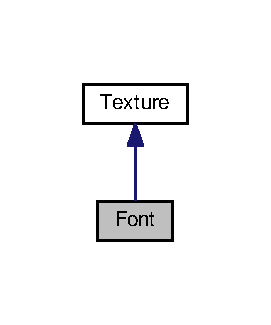
\includegraphics[width=130pt]{classFont__inherit__graph}
\end{center}
\end{figure}


Collaboration diagram for Font\+:\nopagebreak
\begin{figure}[H]
\begin{center}
\leavevmode
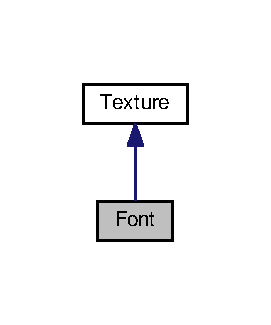
\includegraphics[width=130pt]{classFont__coll__graph}
\end{center}
\end{figure}
\subsection*{Public Member Functions}
\begin{DoxyCompactItemize}
\item 
\hypertarget{classFont_a7ec05e69ec8490a65bb9905d44d57012}{\hyperlink{classFont_a7ec05e69ec8490a65bb9905d44d57012}{Font} (std\+::string const \&fn\+\_\+font, unsigned int taille)}\label{classFont_a7ec05e69ec8490a65bb9905d44d57012}

\begin{DoxyCompactList}\small\item\em Construit une police à partir du fichier fn\+\_\+font. \end{DoxyCompactList}\item 
\hypertarget{classFont_a28cfa9fa2ad26801f300007ad7ef52a0}{void \hyperlink{classFont_a28cfa9fa2ad26801f300007ad7ef52a0}{create\+Text} (std\+::string const \&text, S\+D\+L\+\_\+\+Color color)}\label{classFont_a28cfa9fa2ad26801f300007ad7ef52a0}

\begin{DoxyCompactList}\small\item\em Crée les objets G\+L à partir du texte et de la couleur en argument. \end{DoxyCompactList}\item 
\hypertarget{classFont_a0eb98cf6abe4b13b39d677913da7d209}{void \hyperlink{classFont_a0eb98cf6abe4b13b39d677913da7d209}{create\+Text\+With\+Background} (std\+::string const \&text, S\+D\+L\+\_\+\+Color text\+Color, S\+D\+L\+\_\+\+Color background\+Color)}\label{classFont_a0eb98cf6abe4b13b39d677913da7d209}

\begin{DoxyCompactList}\small\item\em Crée les objets G\+L à partir du texte et de la couleur en argument avec une couleur de fond. \end{DoxyCompactList}\item 
\hypertarget{classFont_a134aaa2f78af0c12d3ce504957169768}{\hyperlink{classFont_a134aaa2f78af0c12d3ce504957169768}{$\sim$\+Font} ()}\label{classFont_a134aaa2f78af0c12d3ce504957169768}

\begin{DoxyCompactList}\small\item\em Destructeur. \end{DoxyCompactList}\item 
\hypertarget{classFont_a50481f4b9b551b4b4fcf45e9dee43658}{unsigned int \hyperlink{classFont_a50481f4b9b551b4b4fcf45e9dee43658}{get\+Height} ()}\label{classFont_a50481f4b9b551b4b4fcf45e9dee43658}

\begin{DoxyCompactList}\small\item\em Retourne la hauteur du texte généré \end{DoxyCompactList}\item 
\hypertarget{classFont_aea596fdec8f7f754d90bac37013686bf}{unsigned int \hyperlink{classFont_aea596fdec8f7f754d90bac37013686bf}{get\+Width} ()}\label{classFont_aea596fdec8f7f754d90bac37013686bf}

\begin{DoxyCompactList}\small\item\em Retourne la largeur du texte généré \end{DoxyCompactList}\end{DoxyCompactItemize}
\subsection*{Additional Inherited Members}


\subsection{Detailed Description}
Gère la conversion de texte en texture G\+L à partir d'une police. 

The documentation for this class was generated from the following files\+:\begin{DoxyCompactItemize}
\item 
\hyperlink{Font_8h}{Font.\+h}\item 
Font.\+cpp\end{DoxyCompactItemize}

\hypertarget{classGuiFactory}{\section{Gui\-Factory Class Reference}
\label{classGuiFactory}\index{Gui\-Factory@{Gui\-Factory}}
}


Classe de création d'objets 2\-D \-: contient les shaders d'affichage 2\-D.  




{\ttfamily \#include $<$Gui\-Factory.\-h$>$}

\subsection*{Public Member Functions}
\begin{DoxyCompactItemize}
\item 
\hypertarget{classGuiFactory_a3d7afcd225a44171f4107d67fdfda2c5}{\hyperlink{classGuiFactory_a3d7afcd225a44171f4107d67fdfda2c5}{Gui\-Factory} ()}\label{classGuiFactory_a3d7afcd225a44171f4107d67fdfda2c5}

\begin{DoxyCompactList}\small\item\em Constructeur. \end{DoxyCompactList}\item 
\hypertarget{classGuiFactory_a77f5f87312431f37b1c279db09b00a46}{\hyperlink{classGuiFactory_a77f5f87312431f37b1c279db09b00a46}{$\sim$\-Gui\-Factory} ()}\label{classGuiFactory_a77f5f87312431f37b1c279db09b00a46}

\begin{DoxyCompactList}\small\item\em Destructeur. \end{DoxyCompactList}\item 
\hypertarget{classGuiFactory_ae37a3ad8191728d30ab050aec876787e}{\hyperlink{classLabel}{Label} $\ast$ \hyperlink{classGuiFactory_ae37a3ad8191728d30ab050aec876787e}{create\-Label} (glm\-::vec2 const \&position, std\-::string const \&font)}\label{classGuiFactory_ae37a3ad8191728d30ab050aec876787e}

\begin{DoxyCompactList}\small\item\em Creation d'un label (texte) \end{DoxyCompactList}\end{DoxyCompactItemize}


\subsection{Detailed Description}
Classe de création d'objets 2\-D \-: contient les shaders d'affichage 2\-D. 

The documentation for this class was generated from the following files\-:\begin{DoxyCompactItemize}
\item 
\hyperlink{GuiFactory_8h}{Gui\-Factory.\-h}\item 
Gui\-Factory.\-cpp\end{DoxyCompactItemize}

\hypertarget{classInput}{\section{Input Class Reference}
\label{classInput}\index{Input@{Input}}
}


gestion des évênements  




{\ttfamily \#include $<$Input.\-h$>$}

\subsection*{Public Member Functions}
\begin{DoxyCompactItemize}
\item 
\hyperlink{classInput_abae3f379d3f157cf42dc857309832dba}{Input} ()
\begin{DoxyCompactList}\small\item\em Constructeur. \end{DoxyCompactList}\item 
\hypertarget{classInput_aa7fe26710dd863d11737bf2f6de4ad05}{void \hyperlink{classInput_aa7fe26710dd863d11737bf2f6de4ad05}{update} ()}\label{classInput_aa7fe26710dd863d11737bf2f6de4ad05}

\begin{DoxyCompactList}\small\item\em Mise à jour des évênements. \end{DoxyCompactList}\item 
\hypertarget{classInput_adafc672c3b01194f8adfc120da0d00fe}{bool \hyperlink{classInput_adafc672c3b01194f8adfc120da0d00fe}{get\-Key} (const S\-D\-L\-\_\-\-Scancode i) const }\label{classInput_adafc672c3b01194f8adfc120da0d00fe}

\begin{DoxyCompactList}\small\item\em Renvoie true si la touche i est enfoncée false sinon. \end{DoxyCompactList}\item 
\hypertarget{classInput_a23a27890996e4b7af907098d9cb896d7}{bool \hyperlink{classInput_a23a27890996e4b7af907098d9cb896d7}{get\-Key\-Release} (const S\-D\-L\-\_\-\-Scancode i) const }\label{classInput_a23a27890996e4b7af907098d9cb896d7}

\begin{DoxyCompactList}\small\item\em Renvoie true si la touche i est relachée false sinon. \end{DoxyCompactList}\item 
\hypertarget{classInput_af6198fd243064d36ab465baa06b039e1}{bool \hyperlink{classInput_af6198fd243064d36ab465baa06b039e1}{mouse\-Move} () const }\label{classInput_af6198fd243064d36ab465baa06b039e1}

\begin{DoxyCompactList}\small\item\em Renvoie true si la souris a bougé false sinon. \end{DoxyCompactList}\item 
\hypertarget{classInput_ae1d91a39827387378f2aa7152fdcc482}{bool \hyperlink{classInput_ae1d91a39827387378f2aa7152fdcc482}{get\-Mouse\-Button} (Uint8 i) const }\label{classInput_ae1d91a39827387378f2aa7152fdcc482}

\begin{DoxyCompactList}\small\item\em Renvoie true si le bouton de souris i est enfoncé false sinon. \end{DoxyCompactList}\item 
\hypertarget{classInput_abb05d3dadc328f090cbf71088691bade}{bool \hyperlink{classInput_abb05d3dadc328f090cbf71088691bade}{get\-Mouse\-Button\-Release} (Uint8 i) const }\label{classInput_abb05d3dadc328f090cbf71088691bade}

\begin{DoxyCompactList}\small\item\em Renvoie true si le bouton de souris i est relaché false sinon. \end{DoxyCompactList}\item 
\hypertarget{classInput_a0bda65e8c8f6511c5ed44c38b95ed0a3}{int \hyperlink{classInput_a0bda65e8c8f6511c5ed44c38b95ed0a3}{get\-X\-Rel} () const }\label{classInput_a0bda65e8c8f6511c5ed44c38b95ed0a3}

\begin{DoxyCompactList}\small\item\em Renvoie le deplacement horizontal de la souris. \end{DoxyCompactList}\item 
\hypertarget{classInput_ad761d98ab768e78ce12a5601ba220f06}{int \hyperlink{classInput_ad761d98ab768e78ce12a5601ba220f06}{get\-Y\-Rel} () const }\label{classInput_ad761d98ab768e78ce12a5601ba220f06}

\begin{DoxyCompactList}\small\item\em Renvoie le deplacement vertical de la souris. \end{DoxyCompactList}\item 
\hypertarget{classInput_a2d977cfea35296f15cd55829f99be9a4}{bool \hyperlink{classInput_a2d977cfea35296f15cd55829f99be9a4}{terminer} () const }\label{classInput_a2d977cfea35296f15cd55829f99be9a4}

\begin{DoxyCompactList}\small\item\em Renvoie true si le programme doit se terminer. \end{DoxyCompactList}\end{DoxyCompactItemize}


\subsection{Detailed Description}
gestion des évênements 

\subsection{Constructor \& Destructor Documentation}
\hypertarget{classInput_abae3f379d3f157cf42dc857309832dba}{\index{Input@{Input}!Input@{Input}}
\index{Input@{Input}!Input@{Input}}
\subsubsection[{Input}]{\setlength{\rightskip}{0pt plus 5cm}Input\-::\-Input (
\begin{DoxyParamCaption}
{}
\end{DoxyParamCaption}
)}}\label{classInput_abae3f379d3f157cf42dc857309832dba}


Constructeur. 

Destructeur. 

The documentation for this class was generated from the following files\-:\begin{DoxyCompactItemize}
\item 
\hyperlink{Input_8h}{Input.\-h}\item 
Input.\-cpp\end{DoxyCompactItemize}

\hypertarget{classLabel}{\section{Label Class Reference}
\label{classLabel}\index{Label@{Label}}
}


Représente un objet Texte 2\-D.  




{\ttfamily \#include $<$Label.\-h$>$}

Inheritance diagram for Label\-:\begin{figure}[H]
\begin{center}
\leavevmode
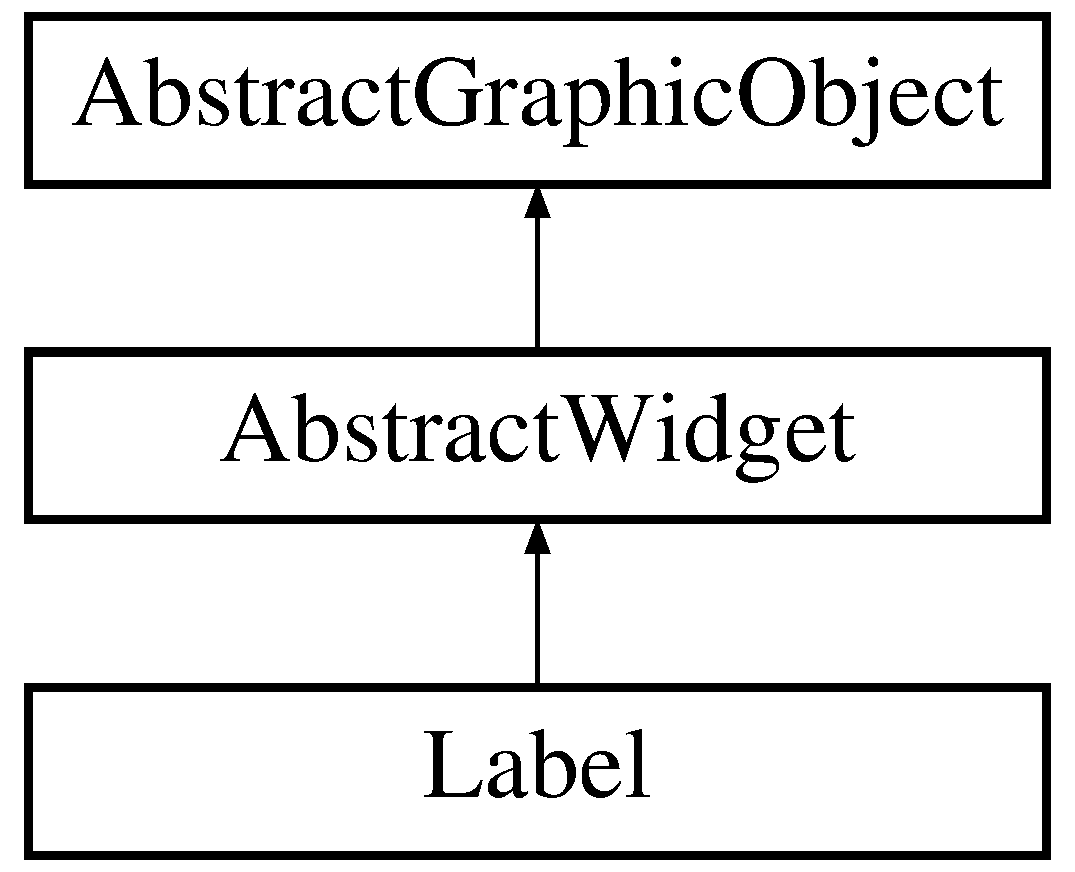
\includegraphics[height=3.000000cm]{classLabel}
\end{center}
\end{figure}
\subsection*{Public Member Functions}
\begin{DoxyCompactItemize}
\item 
\hypertarget{classLabel_a89439b76cefcfc6b560c2920e987072a}{\hyperlink{classLabel_a89439b76cefcfc6b560c2920e987072a}{Label} (std\-::string const \&font, unsigned int taille\-Font, \hyperlink{classShader}{Shader} $\ast$shad, glm\-::vec2 const \&position)}\label{classLabel_a89439b76cefcfc6b560c2920e987072a}

\begin{DoxyCompactList}\small\item\em Constructeur+. \end{DoxyCompactList}\item 
\hypertarget{classLabel_a39e1167a9b5827afd888780973d88894}{virtual \hyperlink{classLabel_a39e1167a9b5827afd888780973d88894}{$\sim$\-Label} ()}\label{classLabel_a39e1167a9b5827afd888780973d88894}

\begin{DoxyCompactList}\small\item\em Destructeur. \end{DoxyCompactList}\item 
\hypertarget{classLabel_a60d568210a67b61388a47fca5326beee}{void \hyperlink{classLabel_a60d568210a67b61388a47fca5326beee}{load} (G\-Lenum drawing\-Method)}\label{classLabel_a60d568210a67b61388a47fca5326beee}

\begin{DoxyCompactList}\small\item\em Génération des objets Open\-G\-L. \end{DoxyCompactList}\item 
\hypertarget{classLabel_ae8ac49d6d22dc837418dce2ea3c01637}{virtual void \hyperlink{classLabel_ae8ac49d6d22dc837418dce2ea3c01637}{draw} (glm\-::mat4 ortho)}\label{classLabel_ae8ac49d6d22dc837418dce2ea3c01637}

\begin{DoxyCompactList}\small\item\em Affichage du label. \end{DoxyCompactList}\item 
\hypertarget{classLabel_afe0eb04dde9253dae986980ab7af5e28}{virtual void \hyperlink{classLabel_afe0eb04dde9253dae986980ab7af5e28}{clean\-Up} ()}\label{classLabel_afe0eb04dde9253dae986980ab7af5e28}

\begin{DoxyCompactList}\small\item\em Détruit les objets de construction intermédiaires. \end{DoxyCompactList}\item 
\hypertarget{classLabel_a2691251a8ef0e53e31438feb5606ec35}{void \hyperlink{classLabel_a2691251a8ef0e53e31438feb5606ec35}{set\-Text} (std\-::string const \&text, S\-D\-L\-\_\-\-Color const \&color, float taille, G\-Lenum drawing\-Method)}\label{classLabel_a2691251a8ef0e53e31438feb5606ec35}

\begin{DoxyCompactList}\small\item\em Changement du texte et regénération. \end{DoxyCompactList}\item 
\hypertarget{classLabel_abf96331e65169cd9855dd3690da9de2b}{void \hyperlink{classLabel_abf96331e65169cd9855dd3690da9de2b}{load} ()}\label{classLabel_abf96331e65169cd9855dd3690da9de2b}

\begin{DoxyCompactList}\small\item\em Génère les objets opengl (vbo,vao,textures) pour cet objet graphique. \end{DoxyCompactList}\end{DoxyCompactItemize}
\subsection*{Protected Attributes}
\begin{DoxyCompactItemize}
\item 
\hypertarget{classLabel_a7f03adffc29da896d49f36d23a72c9b6}{std\-::vector$<$ float $>$ \hyperlink{classLabel_a7f03adffc29da896d49f36d23a72c9b6}{m\-\_\-coord\-Tex}}\label{classLabel_a7f03adffc29da896d49f36d23a72c9b6}

\begin{DoxyCompactList}\small\item\em Tableau temporaire de coordonnées de texture. \end{DoxyCompactList}\item 
\hypertarget{classLabel_a8661786a76b31418bc167e1e48b44ac8}{\hyperlink{classFont}{Font} \hyperlink{classLabel_a8661786a76b31418bc167e1e48b44ac8}{m\-\_\-font}}\label{classLabel_a8661786a76b31418bc167e1e48b44ac8}

\begin{DoxyCompactList}\small\item\em Gestion du texte. \end{DoxyCompactList}\item 
\hypertarget{classLabel_a29541e67ad5511df91e29ac41fe29aa7}{unsigned int \hyperlink{classLabel_a29541e67ad5511df91e29ac41fe29aa7}{m\-\_\-taille\-Font}}\label{classLabel_a29541e67ad5511df91e29ac41fe29aa7}

\begin{DoxyCompactList}\small\item\em Taille de la police. \end{DoxyCompactList}\end{DoxyCompactItemize}


\subsection{Detailed Description}
Représente un objet Texte 2\-D. 

The documentation for this class was generated from the following files\-:\begin{DoxyCompactItemize}
\item 
\hyperlink{Label_8h}{Label.\-h}\item 
Label.\-cpp\end{DoxyCompactItemize}

\hypertarget{classMesh3DS}{\section{Mesh3\-D\-S Class Reference}
\label{classMesh3DS}\index{Mesh3\-D\-S@{Mesh3\-D\-S}}
}


Mesh d'un modèle 3\-D\-S.  




{\ttfamily \#include $<$Mesh3\-D\-S.\-h$>$}

Inheritance diagram for Mesh3\-D\-S\-:\begin{figure}[H]
\begin{center}
\leavevmode
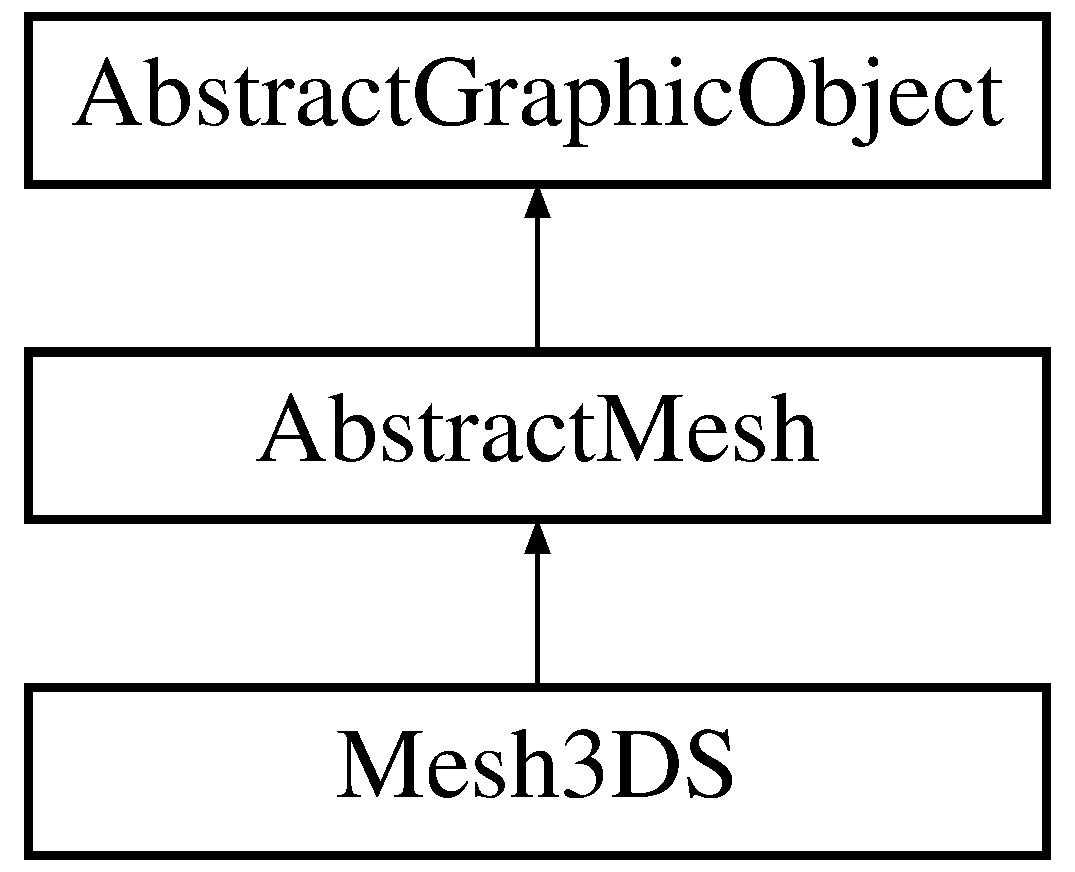
\includegraphics[height=3.000000cm]{classMesh3DS}
\end{center}
\end{figure}
\subsection*{Public Member Functions}
\begin{DoxyCompactItemize}
\item 
\hypertarget{classMesh3DS_abdfac0ddfc9dd72b5bc3504996c07a1c}{\hyperlink{classMesh3DS_abdfac0ddfc9dd72b5bc3504996c07a1c}{Mesh3\-D\-S} ()}\label{classMesh3DS_abdfac0ddfc9dd72b5bc3504996c07a1c}

\begin{DoxyCompactList}\small\item\em Constructeur. \end{DoxyCompactList}\item 
\hypertarget{classMesh3DS_a56ab33cfc6d63a288226993f96b85af8}{\hyperlink{classMesh3DS_a56ab33cfc6d63a288226993f96b85af8}{$\sim$\-Mesh3\-D\-S} ()}\label{classMesh3DS_a56ab33cfc6d63a288226993f96b85af8}

\begin{DoxyCompactList}\small\item\em Destructeur. \end{DoxyCompactList}\item 
\hypertarget{classMesh3DS_a15725546099ea3a351229d875738803d}{bool \hyperlink{classMesh3DS_a15725546099ea3a351229d875738803d}{extract} (Lib3ds\-File $\ast$file3\-D\-S, Lib3ds\-Mesh $\ast$mesh)}\label{classMesh3DS_a15725546099ea3a351229d875738803d}

\begin{DoxyCompactList}\small\item\em Extraction d'un mesh 3\-D\-S. \end{DoxyCompactList}\item 
\hypertarget{classMesh3DS_a0a4b9d9c4be4cd15edb205c52939dd9b}{void \hyperlink{classMesh3DS_a0a4b9d9c4be4cd15edb205c52939dd9b}{extract\-Points} (Lib3ds\-Mesh $\ast$mesh, Lib3ds\-Face $\ast$face)}\label{classMesh3DS_a0a4b9d9c4be4cd15edb205c52939dd9b}

\begin{DoxyCompactList}\small\item\em Extraction des vertices et coordonnées de texture. \end{DoxyCompactList}\item 
\hypertarget{classMesh3DS_a86b0028e6af06db5388bba8d962de91f}{virtual void \hyperlink{classMesh3DS_a86b0028e6af06db5388bba8d962de91f}{load} ()}\label{classMesh3DS_a86b0028e6af06db5388bba8d962de91f}

\begin{DoxyCompactList}\small\item\em Chargement des objets Open\-G\-L. \end{DoxyCompactList}\item 
void \hyperlink{classMesh3DS_a55a5d6856f6d68c38bbc33cf641aa193}{draw} ()
\begin{DoxyCompactList}\small\item\em Affichage. \end{DoxyCompactList}\item 
\hypertarget{classMesh3DS_a366e6d23c347afcc326c83152e8869b1}{virtual void \hyperlink{classMesh3DS_a366e6d23c347afcc326c83152e8869b1}{draw} (glm\-::mat4 mvp)}\label{classMesh3DS_a366e6d23c347afcc326c83152e8869b1}

\begin{DoxyCompactList}\small\item\em Méthode virtuelle pure qui affiche le mesh en fonction de la matrice de modelview\-Projection. \end{DoxyCompactList}\end{DoxyCompactItemize}
\subsection*{Additional Inherited Members}


\subsection{Detailed Description}
Mesh d'un modèle 3\-D\-S. 

\subsection{Member Function Documentation}
\hypertarget{classMesh3DS_a55a5d6856f6d68c38bbc33cf641aa193}{\index{Mesh3\-D\-S@{Mesh3\-D\-S}!draw@{draw}}
\index{draw@{draw}!Mesh3DS@{Mesh3\-D\-S}}
\subsubsection[{draw}]{\setlength{\rightskip}{0pt plus 5cm}void Mesh3\-D\-S\-::draw (
\begin{DoxyParamCaption}
{}
\end{DoxyParamCaption}
)}}\label{classMesh3DS_a55a5d6856f6d68c38bbc33cf641aa193}


Affichage. 

ne fait rien 

The documentation for this class was generated from the following files\-:\begin{DoxyCompactItemize}
\item 
\hyperlink{Mesh3DS_8h}{Mesh3\-D\-S.\-h}\item 
Mesh3\-D\-S.\-cpp\end{DoxyCompactItemize}

\hypertarget{classMeshFactory}{\section{Mesh\+Factory Class Reference}
\label{classMeshFactory}\index{Mesh\+Factory@{Mesh\+Factory}}
}


Classe de gestion des shaders et de génération des modèles 3\+D.  




{\ttfamily \#include $<$Mesh\+Factory.\+h$>$}



Collaboration diagram for Mesh\+Factory\+:\nopagebreak
\begin{figure}[H]
\begin{center}
\leavevmode
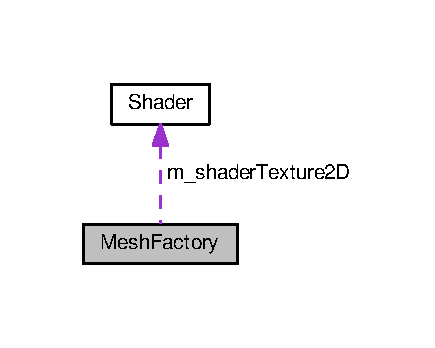
\includegraphics[width=209pt]{classMeshFactory__coll__graph}
\end{center}
\end{figure}
\subsection*{Public Member Functions}
\begin{DoxyCompactItemize}
\item 
\hypertarget{classMeshFactory_a4e7e1572a5d2ce108b5e2c53b58499d2}{\hyperlink{classMeshFactory_a4e7e1572a5d2ce108b5e2c53b58499d2}{Mesh\+Factory} ()}\label{classMeshFactory_a4e7e1572a5d2ce108b5e2c53b58499d2}

\begin{DoxyCompactList}\small\item\em Constructeur. \end{DoxyCompactList}\item 
\hypertarget{classMeshFactory_a642f0dc431ea97f93d3e1cea6df64b8e}{\hyperlink{classMeshFactory_a642f0dc431ea97f93d3e1cea6df64b8e}{$\sim$\+Mesh\+Factory} ()}\label{classMeshFactory_a642f0dc431ea97f93d3e1cea6df64b8e}

\begin{DoxyCompactList}\small\item\em Destructeur. \end{DoxyCompactList}\item 
\hypertarget{classMeshFactory_aed116b3fd378392baa10bae536a83ed4}{\hyperlink{classModel3DS}{Model3\+D\+S} $\ast$ \hyperlink{classMeshFactory_aed116b3fd378392baa10bae536a83ed4}{create3\+D\+S\+Model} (std\+::string const \&model\+Name)}\label{classMeshFactory_aed116b3fd378392baa10bae536a83ed4}

\begin{DoxyCompactList}\small\item\em Création d'un modèle à partir d'un fichier 3\+D\+S M\+A\+X. \end{DoxyCompactList}\item 
\hypertarget{classMeshFactory_a5e35b9f6089ea14c6c9ad88a8ba6f66e}{\hyperlink{classSkybox}{Skybox} $\ast$ \hyperlink{classMeshFactory_a5e35b9f6089ea14c6c9ad88a8ba6f66e}{create\+Skybox} (std\+::string const \&images)}\label{classMeshFactory_a5e35b9f6089ea14c6c9ad88a8ba6f66e}

\begin{DoxyCompactList}\small\item\em Création de l'environnement (simulation de l'espace ici) \end{DoxyCompactList}\item 
\hypertarget{classMeshFactory_a25c338f855f27bd73bbc7bd7b6a1bf7b}{\hyperlink{classSphere}{Sphere} $\ast$ \hyperlink{classMeshFactory_a25c338f855f27bd73bbc7bd7b6a1bf7b}{create\+Planet} (float radius, std\+::string const \&texture)}\label{classMeshFactory_a25c338f855f27bd73bbc7bd7b6a1bf7b}

\begin{DoxyCompactList}\small\item\em Retourne un sphère texturée qui représente une planète. \end{DoxyCompactList}\end{DoxyCompactItemize}
\subsection*{Protected Member Functions}
\begin{DoxyCompactItemize}
\item 
\hypertarget{classMeshFactory_ae8037c270e2e37be03cc5dcc7f5c5d58}{\hyperlink{classTexture}{Texture} $\ast$ \hyperlink{classMeshFactory_ae8037c270e2e37be03cc5dcc7f5c5d58}{get\+Texture} (std\+::string const \&name)}\label{classMeshFactory_ae8037c270e2e37be03cc5dcc7f5c5d58}

\begin{DoxyCompactList}\small\item\em Retourne directement la texture si elle existe déjà sinon la crée puis la retourne. \end{DoxyCompactList}\end{DoxyCompactItemize}
\subsection*{Protected Attributes}
\begin{DoxyCompactItemize}
\item 
\hypertarget{classMeshFactory_a49c1212540dc91ab923efc1d02e305b9}{\hyperlink{classShader}{Shader} $\ast$ \hyperlink{classMeshFactory_a49c1212540dc91ab923efc1d02e305b9}{m\+\_\+shader\+Texture2\+D}}\label{classMeshFactory_a49c1212540dc91ab923efc1d02e305b9}

\begin{DoxyCompactList}\small\item\em Programme shader pour les modèles utilisant des textures 2\+D. \end{DoxyCompactList}\item 
\hypertarget{classMeshFactory_a68d434125dbe5a1c7a7772602d5e77fd}{std\+::map$<$ std\+::string, \hyperlink{classTexture}{Texture} $\ast$ $>$ \hyperlink{classMeshFactory_a68d434125dbe5a1c7a7772602d5e77fd}{m\+\_\+textures}}\label{classMeshFactory_a68d434125dbe5a1c7a7772602d5e77fd}

\begin{DoxyCompactList}\small\item\em Textures gérées directement par la factory (tous sauf 3\+D\+S) \end{DoxyCompactList}\end{DoxyCompactItemize}


\subsection{Detailed Description}
Classe de gestion des shaders et de génération des modèles 3\+D. 

The documentation for this class was generated from the following files\+:\begin{DoxyCompactItemize}
\item 
\hyperlink{MeshFactory_8h}{Mesh\+Factory.\+h}\item 
Mesh\+Factory.\+cpp\end{DoxyCompactItemize}

\hypertarget{classMeshNode}{\section{Mesh\-Node Class Reference}
\label{classMeshNode}\index{Mesh\-Node@{Mesh\-Node}}
}


Classe de gestion de modèles 3\-D.  




{\ttfamily \#include $<$Mesh\-Node.\-h$>$}

\subsection*{Public Member Functions}
\begin{DoxyCompactItemize}
\item 
\hypertarget{classMeshNode_ae0bd876e5fcb2adbf3de54823dedd99e}{\hyperlink{classMeshNode_ae0bd876e5fcb2adbf3de54823dedd99e}{Mesh\-Node} (\hyperlink{classAbstractMesh}{Abstract\-Mesh} $\ast$mesh, glm\-::vec3 position, glm\-::vec3 orientation=glm\-::vec3(0, 0, 0))}\label{classMeshNode_ae0bd876e5fcb2adbf3de54823dedd99e}

\begin{DoxyCompactList}\small\item\em Constructeur. \end{DoxyCompactList}\item 
\hypertarget{classMeshNode_abf8b858b11632dc9827b3ffa1cdc8c9b}{\hyperlink{classMeshNode_abf8b858b11632dc9827b3ffa1cdc8c9b}{$\sim$\-Mesh\-Node} ()}\label{classMeshNode_abf8b858b11632dc9827b3ffa1cdc8c9b}

\begin{DoxyCompactList}\small\item\em Constructeur. \end{DoxyCompactList}\item 
\hypertarget{classMeshNode_af597b2103f1cf7b226b2171474005cdc}{void \hyperlink{classMeshNode_af597b2103f1cf7b226b2171474005cdc}{set\-Position} (glm\-::vec3 const \&position)}\label{classMeshNode_af597b2103f1cf7b226b2171474005cdc}

\begin{DoxyCompactList}\small\item\em Changement de position. \end{DoxyCompactList}\item 
\hypertarget{classMeshNode_a60d28573a39499ea15e6bbc09b3d6c22}{void \hyperlink{classMeshNode_a60d28573a39499ea15e6bbc09b3d6c22}{set\-Orientation} (glm\-::vec3 const \&orientation)}\label{classMeshNode_a60d28573a39499ea15e6bbc09b3d6c22}

\begin{DoxyCompactList}\small\item\em Changement d'orientation. \end{DoxyCompactList}\item 
\hypertarget{classMeshNode_afead0fffba17459bbd07ffb2ff36cd6f}{void \hyperlink{classMeshNode_afead0fffba17459bbd07ffb2ff36cd6f}{set\-Rotation\-Matrix} (glm\-::mat4 const \&rot\-Mat)}\label{classMeshNode_afead0fffba17459bbd07ffb2ff36cd6f}

\begin{DoxyCompactList}\small\item\em Changement de la matrice de rotation. \end{DoxyCompactList}\item 
\hypertarget{classMeshNode_a7b395032fec02d7164791cee62429a37}{void \hyperlink{classMeshNode_a7b395032fec02d7164791cee62429a37}{draw} (glm\-::mat4 const \&projection, glm\-::mat4 const \&modelview)}\label{classMeshNode_a7b395032fec02d7164791cee62429a37}

\begin{DoxyCompactList}\small\item\em Affiche le modèle 3\-D associé \end{DoxyCompactList}\item 
\hypertarget{classMeshNode_a9f798b9773b027539a07d34db4861498}{glm\-::vec3 \hyperlink{classMeshNode_a9f798b9773b027539a07d34db4861498}{get\-Position} () const }\label{classMeshNode_a9f798b9773b027539a07d34db4861498}

\begin{DoxyCompactList}\small\item\em Retourne la position du \hyperlink{classMeshNode}{Mesh\-Node}. \end{DoxyCompactList}\item 
\hypertarget{classMeshNode_afddcbcd339487cf95e0b4078caedbd31}{glm\-::vec3 \hyperlink{classMeshNode_afddcbcd339487cf95e0b4078caedbd31}{get\-Orientation} () const }\label{classMeshNode_afddcbcd339487cf95e0b4078caedbd31}

\begin{DoxyCompactList}\small\item\em retourne l'orientation du \hyperlink{classMeshNode}{Mesh\-Node} \end{DoxyCompactList}\end{DoxyCompactItemize}


\subsection{Detailed Description}
Classe de gestion de modèles 3\-D. 

The documentation for this class was generated from the following files\-:\begin{DoxyCompactItemize}
\item 
\hyperlink{MeshNode_8h}{Mesh\-Node.\-h}\item 
Mesh\-Node.\-cpp\end{DoxyCompactItemize}

\hypertarget{classModel3DS}{\section{Model3\+D\+S Class Reference}
\label{classModel3DS}\index{Model3\+D\+S@{Model3\+D\+S}}
}


Gestion des modèle 3\+D\+S.  




{\ttfamily \#include $<$Model3\+D\+S.\+h$>$}



Inheritance diagram for Model3\+D\+S\+:\nopagebreak
\begin{figure}[H]
\begin{center}
\leavevmode
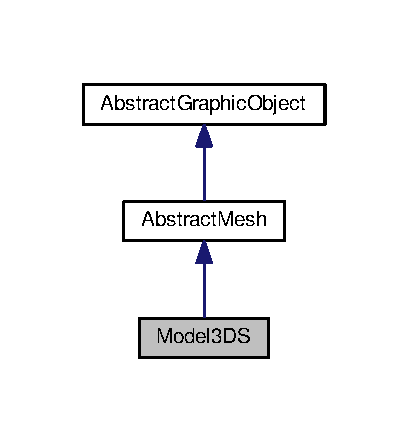
\includegraphics[width=196pt]{classModel3DS__inherit__graph}
\end{center}
\end{figure}


Collaboration diagram for Model3\+D\+S\+:\nopagebreak
\begin{figure}[H]
\begin{center}
\leavevmode
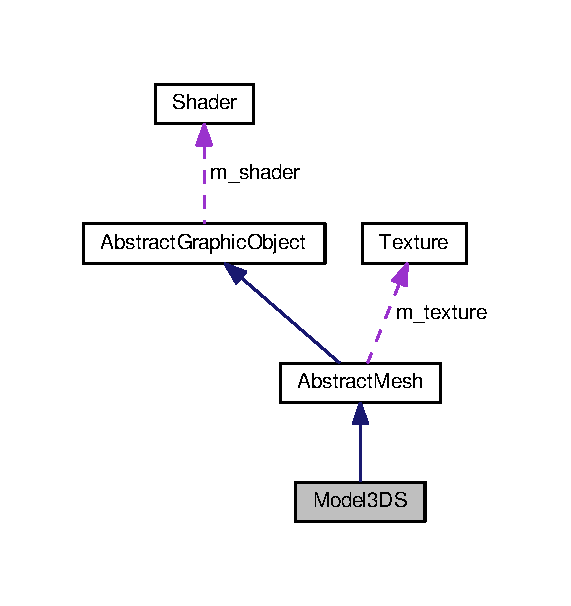
\includegraphics[width=274pt]{classModel3DS__coll__graph}
\end{center}
\end{figure}
\subsection*{Public Member Functions}
\begin{DoxyCompactItemize}
\item 
\hypertarget{classModel3DS_ad40489eb8948fbc5e838333763ed8729}{\hyperlink{classModel3DS_ad40489eb8948fbc5e838333763ed8729}{Model3\+D\+S} (std\+::string const \&file\+\_\+3ds, \hyperlink{classShader}{Shader} $\ast$shader)}\label{classModel3DS_ad40489eb8948fbc5e838333763ed8729}

\begin{DoxyCompactList}\small\item\em Constructeur à partir du fichier 3ds et d'un shader. \end{DoxyCompactList}\item 
\hypertarget{classModel3DS_a87eb706e70138a70745fa866246f24e0}{virtual \hyperlink{classModel3DS_a87eb706e70138a70745fa866246f24e0}{$\sim$\+Model3\+D\+S} ()}\label{classModel3DS_a87eb706e70138a70745fa866246f24e0}

\begin{DoxyCompactList}\small\item\em Destructeur. \end{DoxyCompactList}\item 
\hypertarget{classModel3DS_ad583f00b00866b9b94a352babdf3944a}{virtual void \hyperlink{classModel3DS_ad583f00b00866b9b94a352babdf3944a}{load} ()}\label{classModel3DS_ad583f00b00866b9b94a352babdf3944a}

\begin{DoxyCompactList}\small\item\em Construit les objets Open\+G\+L (vbo et vao) pour ce modèle. \end{DoxyCompactList}\item 
\hypertarget{classModel3DS_ad9566a257fe27a740ee44b1cedbedcd1}{virtual void \hyperlink{classModel3DS_ad9566a257fe27a740ee44b1cedbedcd1}{draw} (glm\+::mat4 mvp)}\label{classModel3DS_ad9566a257fe27a740ee44b1cedbedcd1}

\begin{DoxyCompactList}\small\item\em Affichage. \end{DoxyCompactList}\end{DoxyCompactItemize}
\subsection*{Additional Inherited Members}


\subsection{Detailed Description}
Gestion des modèle 3\+D\+S. 

The documentation for this class was generated from the following files\+:\begin{DoxyCompactItemize}
\item 
\hyperlink{Model3DS_8h}{Model3\+D\+S.\+h}\item 
Model3\+D\+S.\+cpp\end{DoxyCompactItemize}

\hypertarget{classSceneManager}{\section{Scene\+Manager Class Reference}
\label{classSceneManager}\index{Scene\+Manager@{Scene\+Manager}}
}


Gestionnaire des modèle, des caméras (pour le 3\+D) et de l'affichage.  




{\ttfamily \#include $<$Scene\+Manager.\+h$>$}

\subsection*{Public Member Functions}
\begin{DoxyCompactItemize}
\item 
\hypertarget{classSceneManager_a3e4b3a27b84b69d07ed90474ec9c1a93}{\hyperlink{classSceneManager_a3e4b3a27b84b69d07ed90474ec9c1a93}{Scene\+Manager} (int h)}\label{classSceneManager_a3e4b3a27b84b69d07ed90474ec9c1a93}

\begin{DoxyCompactList}\small\item\em Constucteur. \end{DoxyCompactList}\item 
\hypertarget{classSceneManager_a2bb376a85d29e85f47753e26c7539229}{virtual \hyperlink{classSceneManager_a2bb376a85d29e85f47753e26c7539229}{$\sim$\+Scene\+Manager} ()}\label{classSceneManager_a2bb376a85d29e85f47753e26c7539229}

\begin{DoxyCompactList}\small\item\em Constucteur. \end{DoxyCompactList}\item 
\hypertarget{classSceneManager_a28285bcb48151c06270333d39800d100}{\hyperlink{classMeshNode}{Mesh\+Node} $\ast$ \hyperlink{classSceneManager_a28285bcb48151c06270333d39800d100}{add\+Mesh\+Node} (\hyperlink{classAbstractMesh}{Abstract\+Mesh} $\ast$mesh, glm\+::vec3 const \&position, glm\+::vec3 const \&orientation=glm\+::vec3(0, 0, 0))}\label{classSceneManager_a28285bcb48151c06270333d39800d100}

\begin{DoxyCompactList}\small\item\em Ajout d'un modèle 3\+D dans la scene, renvoie le \hyperlink{classMeshNode}{Mesh\+Node} créé \end{DoxyCompactList}\item 
\hypertarget{classSceneManager_a0a09312366326529be7146f5825f703e}{void \hyperlink{classSceneManager_a0a09312366326529be7146f5825f703e}{add\+Widget} (\hyperlink{classAbstractWidget}{Abstract\+Widget} $\ast$wid)}\label{classSceneManager_a0a09312366326529be7146f5825f703e}

\begin{DoxyCompactList}\small\item\em Ajout d'un modèle 2\+D sur l'écran. \end{DoxyCompactList}\item 
\hypertarget{classSceneManager_a85be3bf568c2050211027b9db5e0ffc2}{void \hyperlink{classSceneManager_a85be3bf568c2050211027b9db5e0ffc2}{init3\+D} (int w, int h)}\label{classSceneManager_a85be3bf568c2050211027b9db5e0ffc2}

\begin{DoxyCompactList}\small\item\em Initialisation des modèles 3\+D et de la caméra. \end{DoxyCompactList}\item 
\hypertarget{classSceneManager_af50c8abaae0774c3ded179269fb4f247}{void \hyperlink{classSceneManager_af50c8abaae0774c3ded179269fb4f247}{init2\+D} ()}\label{classSceneManager_af50c8abaae0774c3ded179269fb4f247}

\begin{DoxyCompactList}\small\item\em Initialisation des objets 2\+D et de la matrice orthogonale. \end{DoxyCompactList}\item 
\hypertarget{classSceneManager_a6c3b7f01e718505c424e97bef4bc9394}{void \hyperlink{classSceneManager_a6c3b7f01e718505c424e97bef4bc9394}{init\+Sounds} ()}\label{classSceneManager_a6c3b7f01e718505c424e97bef4bc9394}

\begin{DoxyCompactList}\small\item\em Initialisation des musiques et des effets sonores. \end{DoxyCompactList}\item 
\hypertarget{classSceneManager_ae95a2a4d00b37f18b924f30570619a30}{void \hyperlink{classSceneManager_ae95a2a4d00b37f18b924f30570619a30}{draw\+All} ()}\label{classSceneManager_ae95a2a4d00b37f18b924f30570619a30}

\begin{DoxyCompactList}\small\item\em Affichage de tous les modèles. \end{DoxyCompactList}\item 
\hypertarget{classSceneManager_a167d8c660828c07aa6b189e0a4c809bd}{void \hyperlink{classSceneManager_a167d8c660828c07aa6b189e0a4c809bd}{on\+Pre\+Render} ()}\label{classSceneManager_a167d8c660828c07aa6b189e0a4c809bd}

\begin{DoxyCompactList}\small\item\em Avant le rendu. \end{DoxyCompactList}\item 
\hypertarget{classSceneManager_abbdf898b3f5161018bbc2761fa6a49dd}{bool \hyperlink{classSceneManager_abbdf898b3f5161018bbc2761fa6a49dd}{execute} (S\+D\+L\+\_\+\+Window $\ast$window, unsigned int w, unsigned int h)}\label{classSceneManager_abbdf898b3f5161018bbc2761fa6a49dd}

\begin{DoxyCompactList}\small\item\em Exécution de la boucle principale. \end{DoxyCompactList}\item 
\hypertarget{classSceneManager_ab063fdc682ba6a8abe4a02a228f27aab}{void \hyperlink{classSceneManager_ab063fdc682ba6a8abe4a02a228f27aab}{update\+Cameras} ()}\label{classSceneManager_ab063fdc682ba6a8abe4a02a228f27aab}

\begin{DoxyCompactList}\small\item\em Déplace les caméras et met à jour les matrices. \end{DoxyCompactList}\item 
\hypertarget{classSceneManager_a153fdb0850c95f9c75730a9e76fbd7e0}{void \hyperlink{classSceneManager_a153fdb0850c95f9c75730a9e76fbd7e0}{change\+Camera} ()}\label{classSceneManager_a153fdb0850c95f9c75730a9e76fbd7e0}

\begin{DoxyCompactList}\small\item\em Change de caméra active. \end{DoxyCompactList}\end{DoxyCompactItemize}


\subsection{Detailed Description}
Gestionnaire des modèle, des caméras (pour le 3\+D) et de l'affichage. 

The documentation for this class was generated from the following files\+:\begin{DoxyCompactItemize}
\item 
\hyperlink{SceneManager_8h}{Scene\+Manager.\+h}\item 
Scene\+Manager.\+cpp\end{DoxyCompactItemize}

\hypertarget{classShader}{\section{Shader Class Reference}
\label{classShader}\index{Shader@{Shader}}
}


Classe de gestion de programmes shaders (compilation, édition de liens, contrôle et destruction)  




{\ttfamily \#include $<$Shader.\-h$>$}

\subsection*{Public Member Functions}
\begin{DoxyCompactItemize}
\item 
\hypertarget{classShader_a85497d4a14f30f3518cf096a19ffdfa9}{\hyperlink{classShader_a85497d4a14f30f3518cf096a19ffdfa9}{Shader} (std\-::string const \&vertex\-Shader, std\-::string const \&fragment\-Shader)}\label{classShader_a85497d4a14f30f3518cf096a19ffdfa9}

\begin{DoxyCompactList}\small\item\em Constructeur à partir d'un fichier vertex\-Shader et d'un fichier fragment\-Shader. \end{DoxyCompactList}\item 
\hypertarget{classShader_ac25dbd32c17223c50e045ddbf060f5c1}{\hyperlink{classShader_ac25dbd32c17223c50e045ddbf060f5c1}{Shader} (\hyperlink{classShader}{Shader} const \&shader)}\label{classShader_ac25dbd32c17223c50e045ddbf060f5c1}

\begin{DoxyCompactList}\small\item\em Constructeur de copie d'un shader. \end{DoxyCompactList}\item 
\hypertarget{classShader_aff01df87e8a102f270b5b135a295e59d}{virtual \hyperlink{classShader_aff01df87e8a102f270b5b135a295e59d}{$\sim$\-Shader} ()}\label{classShader_aff01df87e8a102f270b5b135a295e59d}

\begin{DoxyCompactList}\small\item\em Destructeur. \end{DoxyCompactList}\item 
\hypertarget{classShader_a4222b925de192c794cdef621b13a5914}{void \hyperlink{classShader_a4222b925de192c794cdef621b13a5914}{load} ()}\label{classShader_a4222b925de192c794cdef621b13a5914}

\begin{DoxyCompactList}\small\item\em Récupération des sources, compilation et édition de liens. \end{DoxyCompactList}\item 
\hypertarget{classShader_aaa2ce3b8edbb1954b0b627dcb40cff7e}{std\-::string \hyperlink{classShader_aaa2ce3b8edbb1954b0b627dcb40cff7e}{get\-Vertex\-Shader} () const }\label{classShader_aaa2ce3b8edbb1954b0b627dcb40cff7e}

\begin{DoxyCompactList}\small\item\em Retourne le nom du fichier vertex\-Shader. \end{DoxyCompactList}\item 
\hypertarget{classShader_ac5069963469dcac0be6841e73de29aa3}{std\-::string \hyperlink{classShader_ac5069963469dcac0be6841e73de29aa3}{get\-Fragment\-Shader} () const }\label{classShader_ac5069963469dcac0be6841e73de29aa3}

\begin{DoxyCompactList}\small\item\em Retourne le nom du fichier fragment\-Shader. \end{DoxyCompactList}\item 
\hypertarget{classShader_a7caa048bcdc688aba0c691f56bd4c194}{void \hyperlink{classShader_a7caa048bcdc688aba0c691f56bd4c194}{envoyer\-Mat4} (std\-::string const \&nom, glm\-::mat4 const \&matrice)}\label{classShader_a7caa048bcdc688aba0c691f56bd4c194}

\begin{DoxyCompactList}\small\item\em Envoyer une matrice 4x4 comme variable Uniform (commune à toutes les instances de ce shader) \end{DoxyCompactList}\item 
\hypertarget{classShader_acf2af4edd5d98c008b9fd2de3a55c5cf}{void \hyperlink{classShader_acf2af4edd5d98c008b9fd2de3a55c5cf}{begin} ()}\label{classShader_acf2af4edd5d98c008b9fd2de3a55c5cf}

\begin{DoxyCompactList}\small\item\em Début du rendu \-: à appeler avant le rendu d'un objet pour utiliser ce shader pour son affichage. \end{DoxyCompactList}\item 
\hypertarget{classShader_abfff82b6778a0b6d1f1a599b1b306b1d}{void \hyperlink{classShader_abfff82b6778a0b6d1f1a599b1b306b1d}{end} ()}\label{classShader_abfff82b6778a0b6d1f1a599b1b306b1d}

\begin{DoxyCompactList}\small\item\em À appeler après le rendu d'un objet ne plus utiliser ce shader. \end{DoxyCompactList}\item 
\hypertarget{classShader_aae9136479d5affe1b14f1c79efe79600}{bool \hyperlink{classShader_aae9136479d5affe1b14f1c79efe79600}{is\-Program} ()}\label{classShader_aae9136479d5affe1b14f1c79efe79600}

\begin{DoxyCompactList}\small\item\em Renvoie true si le programme shader est valide false sinon. \end{DoxyCompactList}\item 
\hypertarget{classShader_ad1bc9a16400499ec80c4f716a390abaf}{G\-Luint \hyperlink{classShader_ad1bc9a16400499ec80c4f716a390abaf}{get\-I\-D} ()}\label{classShader_ad1bc9a16400499ec80c4f716a390abaf}

\begin{DoxyCompactList}\small\item\em Renvoie l'identifiant Open\-G\-L de ce shader. \end{DoxyCompactList}\item 
\hypertarget{classShader_aafa6167c1e130229a19a90bee95aaff0}{void {\bfseries load\-Simple} ()}\label{classShader_aafa6167c1e130229a19a90bee95aaff0}

\end{DoxyCompactItemize}


\subsection{Detailed Description}
Classe de gestion de programmes shaders (compilation, édition de liens, contrôle et destruction) 

The documentation for this class was generated from the following files\-:\begin{DoxyCompactItemize}
\item 
\hyperlink{Shader_8h}{Shader.\-h}\item 
Shader.\-cpp\end{DoxyCompactItemize}

\hypertarget{classSkybox}{\section{Skybox Class Reference}
\label{classSkybox}\index{Skybox@{Skybox}}
}


Cube avec textures de ciel plaquées.  




{\ttfamily \#include $<$Skybox.\+h$>$}



Inheritance diagram for Skybox\+:\nopagebreak
\begin{figure}[H]
\begin{center}
\leavevmode
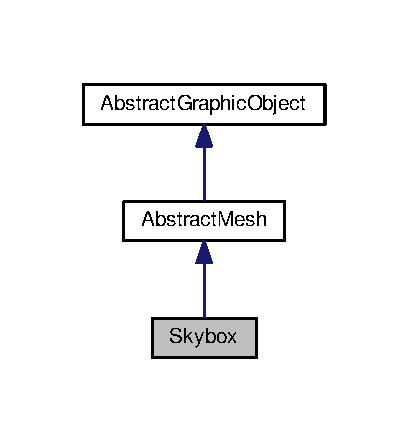
\includegraphics[width=196pt]{classSkybox__inherit__graph}
\end{center}
\end{figure}


Collaboration diagram for Skybox\+:\nopagebreak
\begin{figure}[H]
\begin{center}
\leavevmode
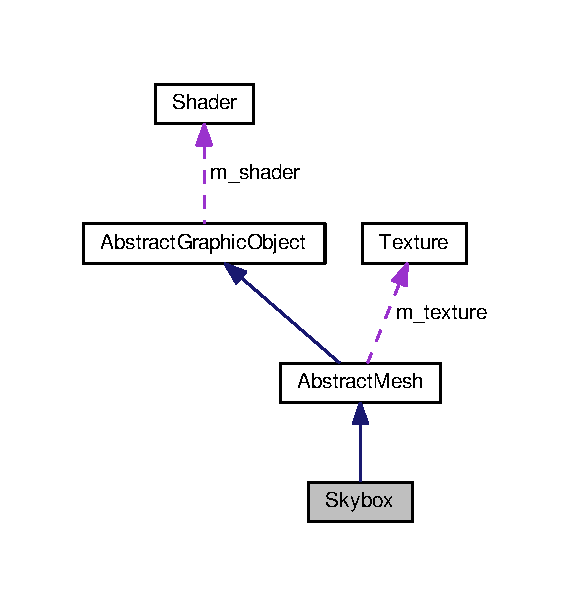
\includegraphics[width=274pt]{classSkybox__coll__graph}
\end{center}
\end{figure}
\subsection*{Public Member Functions}
\begin{DoxyCompactItemize}
\item 
\hypertarget{classSkybox_abe8add7195fe6ac462d83f5afb9d26a6}{\hyperlink{classSkybox_abe8add7195fe6ac462d83f5afb9d26a6}{Skybox} (float taille, \hyperlink{classShader}{Shader} $\ast$shad, \hyperlink{classTexture}{Texture} $\ast$tex)}\label{classSkybox_abe8add7195fe6ac462d83f5afb9d26a6}

\begin{DoxyCompactList}\small\item\em Constructeur pour une skybox mono-\/texturée. \end{DoxyCompactList}\item 
\hypertarget{classSkybox_a62ad4c6b4b1965a0a6d8536a50d4c090}{virtual \hyperlink{classSkybox_a62ad4c6b4b1965a0a6d8536a50d4c090}{$\sim$\+Skybox} ()}\label{classSkybox_a62ad4c6b4b1965a0a6d8536a50d4c090}

\begin{DoxyCompactList}\small\item\em Destructeur. \end{DoxyCompactList}\item 
\hypertarget{classSkybox_a07b12f1abc7c7b344ae5db0e3245d95a}{virtual void \hyperlink{classSkybox_a07b12f1abc7c7b344ae5db0e3245d95a}{draw} (glm\+::mat4 mvp)}\label{classSkybox_a07b12f1abc7c7b344ae5db0e3245d95a}

\begin{DoxyCompactList}\small\item\em Affichage. \end{DoxyCompactList}\end{DoxyCompactItemize}
\subsection*{Additional Inherited Members}


\subsection{Detailed Description}
Cube avec textures de ciel plaquées. 

The documentation for this class was generated from the following files\+:\begin{DoxyCompactItemize}
\item 
\hyperlink{Skybox_8h}{Skybox.\+h}\item 
Skybox.\+cpp\end{DoxyCompactItemize}

\hypertarget{classSoundManager}{\section{Sound\+Manager Class Reference}
\label{classSoundManager}\index{Sound\+Manager@{Sound\+Manager}}
}


Gestionnaire de sons.  




{\ttfamily \#include $<$Sound\+Manager.\+h$>$}

\subsection*{Public Member Functions}
\begin{DoxyCompactItemize}
\item 
\hypertarget{classSoundManager_abcc1fbf3488be5788a42c9a4fe56df35}{\hyperlink{classSoundManager_abcc1fbf3488be5788a42c9a4fe56df35}{Sound\+Manager} ()}\label{classSoundManager_abcc1fbf3488be5788a42c9a4fe56df35}

\begin{DoxyCompactList}\small\item\em Constructeur. \end{DoxyCompactList}\item 
\hypertarget{classSoundManager_ad5dbf8eab22db48ff8f3db51b02f8938}{\hyperlink{classSoundManager_ad5dbf8eab22db48ff8f3db51b02f8938}{$\sim$\+Sound\+Manager} ()}\label{classSoundManager_ad5dbf8eab22db48ff8f3db51b02f8938}

\begin{DoxyCompactList}\small\item\em Constructeur. \end{DoxyCompactList}\item 
\hypertarget{classSoundManager_a6dcfd41960f3034460c601b04a1a1eb7}{void \hyperlink{classSoundManager_a6dcfd41960f3034460c601b04a1a1eb7}{add\+Music} (std\+::string const \&file)}\label{classSoundManager_a6dcfd41960f3034460c601b04a1a1eb7}

\begin{DoxyCompactList}\small\item\em Ajoute une musique à la liste de lecture. \end{DoxyCompactList}\item 
\hypertarget{classSoundManager_adf63b6806ffcc147633d5c3982b3f2ff}{void \hyperlink{classSoundManager_adf63b6806ffcc147633d5c3982b3f2ff}{add\+Effect} (std\+::string const \&name, std\+::string const \&file)}\label{classSoundManager_adf63b6806ffcc147633d5c3982b3f2ff}

\begin{DoxyCompactList}\small\item\em Ajoute un effet à la liste des effets. \end{DoxyCompactList}\item 
\hypertarget{classSoundManager_a43c79a5278a1c423a463eda0c80b8c11}{bool \hyperlink{classSoundManager_a43c79a5278a1c423a463eda0c80b8c11}{is\+Playing\+Music} ()}\label{classSoundManager_a43c79a5278a1c423a463eda0c80b8c11}

\begin{DoxyCompactList}\small\item\em Renvoie true si le gectionnaire de son est en train de jouer une musique false sinon. \end{DoxyCompactList}\item 
\hypertarget{classSoundManager_a22b283e46295d90a28b97df7923f2999}{void \hyperlink{classSoundManager_a22b283e46295d90a28b97df7923f2999}{play\+Music} ()}\label{classSoundManager_a22b283e46295d90a28b97df7923f2999}

\begin{DoxyCompactList}\small\item\em Lit la liste de lecture. \end{DoxyCompactList}\item 
\hypertarget{classSoundManager_aa78ebda8e0a1a06b87d405eda32fa21a}{void \hyperlink{classSoundManager_aa78ebda8e0a1a06b87d405eda32fa21a}{next\+Music} ()}\label{classSoundManager_aa78ebda8e0a1a06b87d405eda32fa21a}

\begin{DoxyCompactList}\small\item\em Lit la musique suivant dans la liste de lecture. \end{DoxyCompactList}\item 
\hypertarget{classSoundManager_a5ae512c899d6cf2e818a0c12e7f74b06}{void \hyperlink{classSoundManager_a5ae512c899d6cf2e818a0c12e7f74b06}{play\+Effect} (std\+::string const \&name, int volume)}\label{classSoundManager_a5ae512c899d6cf2e818a0c12e7f74b06}

\begin{DoxyCompactList}\small\item\em Joue l'effet identifié par son nom. \end{DoxyCompactList}\end{DoxyCompactItemize}


\subsection{Detailed Description}
Gestionnaire de sons. 

The documentation for this class was generated from the following files\+:\begin{DoxyCompactItemize}
\item 
\hyperlink{SoundManager_8h}{Sound\+Manager.\+h}\item 
Sound\+Manager.\+cpp\end{DoxyCompactItemize}

\hypertarget{classSphere}{\section{Sphere Class Reference}
\label{classSphere}\index{Sphere@{Sphere}}
}


Définition d'une sphère texturée.  




{\ttfamily \#include $<$Sphere.\+h$>$}



Inheritance diagram for Sphere\+:\nopagebreak
\begin{figure}[H]
\begin{center}
\leavevmode
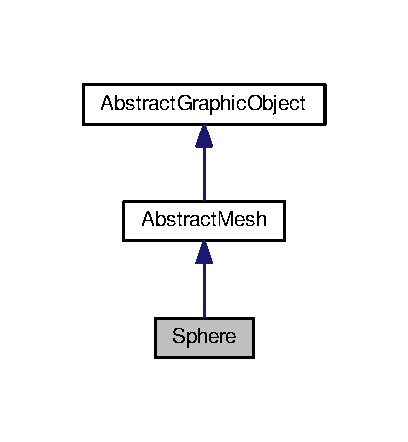
\includegraphics[width=196pt]{classSphere__inherit__graph}
\end{center}
\end{figure}


Collaboration diagram for Sphere\+:\nopagebreak
\begin{figure}[H]
\begin{center}
\leavevmode
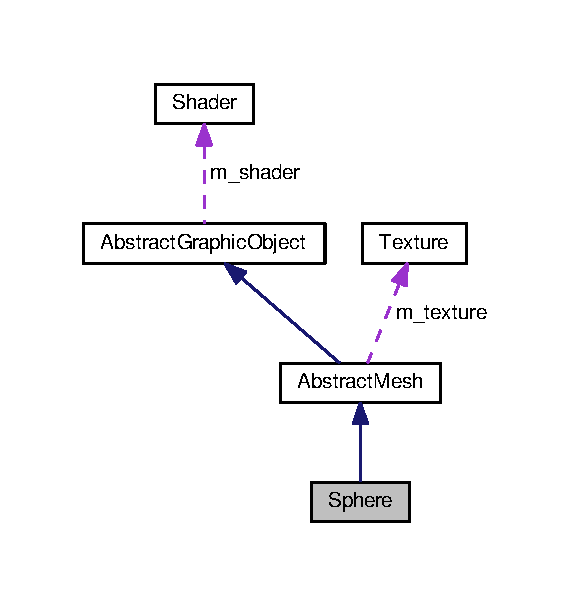
\includegraphics[width=274pt]{classSphere__coll__graph}
\end{center}
\end{figure}
\subsection*{Public Member Functions}
\begin{DoxyCompactItemize}
\item 
\hypertarget{classSphere_a9966f217c4fd4e67f8aac6bac69001dd}{\hyperlink{classSphere_a9966f217c4fd4e67f8aac6bac69001dd}{Sphere} (float radius, unsigned int nb\+Lat, unsigned int nb\+Long, \hyperlink{classShader}{Shader} $\ast$shad, \hyperlink{classTexture}{Texture} $\ast$tex)}\label{classSphere_a9966f217c4fd4e67f8aac6bac69001dd}

\begin{DoxyCompactList}\small\item\em Constructeur. \end{DoxyCompactList}\item 
\hypertarget{classSphere_a569c071e50a3e11f678630ee1a17737e}{\hyperlink{classSphere_a569c071e50a3e11f678630ee1a17737e}{$\sim$\+Sphere} ()}\label{classSphere_a569c071e50a3e11f678630ee1a17737e}

\begin{DoxyCompactList}\small\item\em Destructeur. \end{DoxyCompactList}\item 
\hypertarget{classSphere_a9ae197a2b240049447bb0405a5916072}{void \hyperlink{classSphere_a9ae197a2b240049447bb0405a5916072}{load} ()}\label{classSphere_a9ae197a2b240049447bb0405a5916072}

\begin{DoxyCompactList}\small\item\em Charger les objets G\+L. \end{DoxyCompactList}\item 
\hypertarget{classSphere_a25ad89145b9d03ffb97ef88d4b9598e8}{void \hyperlink{classSphere_a25ad89145b9d03ffb97ef88d4b9598e8}{init\+Sphere} (double r, unsigned int lats, unsigned int longs)}\label{classSphere_a25ad89145b9d03ffb97ef88d4b9598e8}

\begin{DoxyCompactList}\small\item\em Initialisation des vertices et des coordonnées de texture. \end{DoxyCompactList}\item 
\hypertarget{classSphere_a1fea410bb099ab2b60707ed71186c17c}{void \hyperlink{classSphere_a1fea410bb099ab2b60707ed71186c17c}{draw} (glm\+::mat4 mvp)}\label{classSphere_a1fea410bb099ab2b60707ed71186c17c}

\begin{DoxyCompactList}\small\item\em Affichage. \end{DoxyCompactList}\end{DoxyCompactItemize}
\subsection*{Additional Inherited Members}


\subsection{Detailed Description}
Définition d'une sphère texturée. 

The documentation for this class was generated from the following files\+:\begin{DoxyCompactItemize}
\item 
\hyperlink{Sphere_8h}{Sphere.\+h}\item 
Sphere.\+cpp\end{DoxyCompactItemize}

\hypertarget{classTexture}{\section{Texture Class Reference}
\label{classTexture}\index{Texture@{Texture}}
}


Gère les textures Open\+G\+L et leur importation via une image ou une police.  




{\ttfamily \#include $<$Texture.\+h$>$}



Inheritance diagram for Texture\+:\nopagebreak
\begin{figure}[H]
\begin{center}
\leavevmode
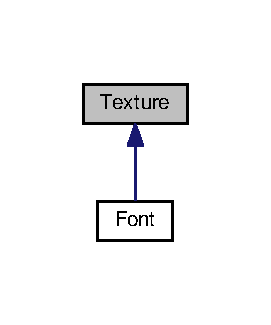
\includegraphics[width=130pt]{classTexture__inherit__graph}
\end{center}
\end{figure}
\subsection*{Public Member Functions}
\begin{DoxyCompactItemize}
\item 
\hypertarget{classTexture_a6c275e3f186675ff6ed73ccf970e552f}{\hyperlink{classTexture_a6c275e3f186675ff6ed73ccf970e552f}{Texture} ()}\label{classTexture_a6c275e3f186675ff6ed73ccf970e552f}

\begin{DoxyCompactList}\small\item\em Contruit une texture vide. \end{DoxyCompactList}\item 
\hypertarget{classTexture_a20743f514b11d6de3ee3a2517fc36c1f}{\hyperlink{classTexture_a20743f514b11d6de3ee3a2517fc36c1f}{Texture} (std\+::string const \&fn)}\label{classTexture_a20743f514b11d6de3ee3a2517fc36c1f}

\begin{DoxyCompactList}\small\item\em Construit une texture à partir d'une image. \end{DoxyCompactList}\item 
\hypertarget{classTexture_abc7ef59dd742a585d2bd1a0c13a7b64f}{\hyperlink{classTexture_abc7ef59dd742a585d2bd1a0c13a7b64f}{Texture} (\hyperlink{classTexture}{Texture} \&tex)}\label{classTexture_abc7ef59dd742a585d2bd1a0c13a7b64f}

\begin{DoxyCompactList}\small\item\em Constructeur de copie. \end{DoxyCompactList}\item 
\hypertarget{classTexture_a09c4bcb7462f64c1d20fa69dba3cee8a}{\hyperlink{classTexture_a09c4bcb7462f64c1d20fa69dba3cee8a}{$\sim$\+Texture} ()}\label{classTexture_a09c4bcb7462f64c1d20fa69dba3cee8a}

\begin{DoxyCompactList}\small\item\em Destructeur. \end{DoxyCompactList}\item 
\hypertarget{classTexture_ad3a36458f5ccd281b964ad1b2b4f92db}{void \hyperlink{classTexture_ad3a36458f5ccd281b964ad1b2b4f92db}{load} ()}\label{classTexture_ad3a36458f5ccd281b964ad1b2b4f92db}

\begin{DoxyCompactList}\small\item\em Création des objets G\+L pour une texture image. \end{DoxyCompactList}\item 
\hypertarget{classTexture_a460d3f86d1add69bd0c81623865b990a}{void \hyperlink{classTexture_a460d3f86d1add69bd0c81623865b990a}{load\+Cull\+Face} ()}\label{classTexture_a460d3f86d1add69bd0c81623865b990a}

\begin{DoxyCompactList}\small\item\em Création des objets G\+L pour une texture image sans répétition. \end{DoxyCompactList}\item 
\hypertarget{classTexture_a006028bb4f1c28b731260ce24a7ba263}{void \hyperlink{classTexture_a006028bb4f1c28b731260ce24a7ba263}{load\+Cubemap} (std\+::vector$<$ std\+::string $>$ faces)}\label{classTexture_a006028bb4f1c28b731260ce24a7ba263}

\begin{DoxyCompactList}\small\item\em Création des objets G\+L pour une texture Cube Map. \end{DoxyCompactList}\item 
\hypertarget{classTexture_a041fd824a637b8c02df9564cb96ee53e}{void \hyperlink{classTexture_a041fd824a637b8c02df9564cb96ee53e}{load\+Empty} (unsigned int width, unsigned int height, G\+Lenum format, G\+Lenum format\+Interne)}\label{classTexture_a041fd824a637b8c02df9564cb96ee53e}

\begin{DoxyCompactList}\small\item\em Création des objets G\+L pour une texture vide. \end{DoxyCompactList}\item 
\hypertarget{classTexture_a18a767fcb0c2648f5c4f3bbc6ac06fc5}{\hyperlink{classTexture}{Texture} \& \hyperlink{classTexture_a18a767fcb0c2648f5c4f3bbc6ac06fc5}{operator=} (\hyperlink{classTexture}{Texture} \&tex)}\label{classTexture_a18a767fcb0c2648f5c4f3bbc6ac06fc5}

\begin{DoxyCompactList}\small\item\em Equivalent au constructeur de copie. \end{DoxyCompactList}\item 
\hypertarget{classTexture_a3840dc7429982ffaddeafc8d62345b5d}{void \hyperlink{classTexture_a3840dc7429982ffaddeafc8d62345b5d}{bind} ()}\label{classTexture_a3840dc7429982ffaddeafc8d62345b5d}

\begin{DoxyCompactList}\small\item\em Verrouillage de la texture (obligatoire pour pouvoir afficher ou modifier les objets G\+L) \end{DoxyCompactList}\item 
\hypertarget{classTexture_a8480eed7ed703a937c3e6ab528f559bd}{void \hyperlink{classTexture_a8480eed7ed703a937c3e6ab528f559bd}{unbind} ()}\label{classTexture_a8480eed7ed703a937c3e6ab528f559bd}

\begin{DoxyCompactList}\small\item\em Verrouillage de la texture (Facultatif) \end{DoxyCompactList}\item 
\hypertarget{classTexture_a29d25e904c47cc08b5420c0cd5474743}{std\+::string \hyperlink{classTexture_a29d25e904c47cc08b5420c0cd5474743}{get\+Name} ()}\label{classTexture_a29d25e904c47cc08b5420c0cd5474743}

\begin{DoxyCompactList}\small\item\em Renvoie le nom du fichier image ou police. \end{DoxyCompactList}\item 
\hypertarget{classTexture_aab4bc3a5783b23881209c15223f2621e}{G\+Luint \hyperlink{classTexture_aab4bc3a5783b23881209c15223f2621e}{get\+I\+D} ()}\label{classTexture_aab4bc3a5783b23881209c15223f2621e}

\begin{DoxyCompactList}\small\item\em Renvoie l'identifiant Open\+G\+L de la texture. \end{DoxyCompactList}\item 
\hypertarget{classTexture_ac6f04a129a2c8ac1e22c7990866849db}{bool \hyperlink{classTexture_ac6f04a129a2c8ac1e22c7990866849db}{is\+Valid} ()}\label{classTexture_ac6f04a129a2c8ac1e22c7990866849db}

\begin{DoxyCompactList}\small\item\em Renvoie true si la police est valide false sinon. \end{DoxyCompactList}\end{DoxyCompactItemize}
\subsection*{Protected Member Functions}
\begin{DoxyCompactItemize}
\item 
\hypertarget{classTexture_a2b28225171c8805005b49ba51647369d}{S\+D\+L\+\_\+\+Surface $\ast$ \hyperlink{classTexture_a2b28225171c8805005b49ba51647369d}{read\+Pixels} ()}\label{classTexture_a2b28225171c8805005b49ba51647369d}

\begin{DoxyCompactList}\small\item\em Retourne une S\+D\+L\+\_\+\+Surface à parir de l'image désignée par m\+\_\+fn. \end{DoxyCompactList}\item 
\hypertarget{classTexture_a7f8771fdac09768ef06643ec314d02fb}{S\+D\+L\+\_\+\+Surface $\ast$ {\bfseries read\+Pixels} (std\+::string image)}\label{classTexture_a7f8771fdac09768ef06643ec314d02fb}

\item 
\hypertarget{classTexture_a176dc762ce2e4e7b81ee05998c79beb3}{S\+D\+L\+\_\+\+Surface $\ast$ \hyperlink{classTexture_a176dc762ce2e4e7b81ee05998c79beb3}{inverse\+Pixels} (S\+D\+L\+\_\+\+Surface $\ast$image\+Source)}\label{classTexture_a176dc762ce2e4e7b81ee05998c79beb3}

\begin{DoxyCompactList}\small\item\em Inverse les pixels pour retourner une image. \end{DoxyCompactList}\item 
\hypertarget{classTexture_ad2c6a0ce24d3b8d092abb39d46c41370}{void \hyperlink{classTexture_ad2c6a0ce24d3b8d092abb39d46c41370}{upload\+To\+G\+P\+U} (S\+D\+L\+\_\+\+Surface $\ast$image)}\label{classTexture_ad2c6a0ce24d3b8d092abb39d46c41370}

\begin{DoxyCompactList}\small\item\em Charge les objets Open\+G\+L pour cette texture. \end{DoxyCompactList}\item 
\hypertarget{classTexture_a206c1f87658e5991b722b120cc380ee2}{void \hyperlink{classTexture_a206c1f87658e5991b722b120cc380ee2}{detect\+Format} (S\+D\+L\+\_\+\+Surface $\ast$image, G\+Lenum \&format\+Interne, G\+Lenum \&format)}\label{classTexture_a206c1f87658e5991b722b120cc380ee2}

\begin{DoxyCompactList}\small\item\em Détecte le format et le format interne d'une image. \end{DoxyCompactList}\end{DoxyCompactItemize}
\subsection*{Protected Attributes}
\begin{DoxyCompactItemize}
\item 
\hypertarget{classTexture_acc091a7a07abe75c263544eaeec44664}{G\+Luint \hyperlink{classTexture_acc091a7a07abe75c263544eaeec44664}{m\+\_\+id}}\label{classTexture_acc091a7a07abe75c263544eaeec44664}

\begin{DoxyCompactList}\small\item\em Identifiant Open\+G\+L pour cette texture. \end{DoxyCompactList}\item 
\hypertarget{classTexture_a9a0d5c5fadadbca3595e46958cc88838}{std\+::string \hyperlink{classTexture_a9a0d5c5fadadbca3595e46958cc88838}{m\+\_\+fn}}\label{classTexture_a9a0d5c5fadadbca3595e46958cc88838}

\begin{DoxyCompactList}\small\item\em Nom du fichier image de cette texture. \end{DoxyCompactList}\item 
\hypertarget{classTexture_a00dc4aaa74b0e979f4f7be844a349c62}{G\+Lenum \hyperlink{classTexture_a00dc4aaa74b0e979f4f7be844a349c62}{m\+\_\+format}}\label{classTexture_a00dc4aaa74b0e979f4f7be844a349c62}

\begin{DoxyCompactList}\small\item\em Format de l'image. \end{DoxyCompactList}\end{DoxyCompactItemize}


\subsection{Detailed Description}
Gère les textures Open\+G\+L et leur importation via une image ou une police. 

The documentation for this class was generated from the following files\+:\begin{DoxyCompactItemize}
\item 
\hyperlink{Texture_8h}{Texture.\+h}\item 
Texture.\+cpp\end{DoxyCompactItemize}

\chapter{File Documentation}
\hypertarget{AbstractButton_8h}{\section{Abstract\+Button.\+h File Reference}
\label{AbstractButton_8h}\index{Abstract\+Button.\+h@{Abstract\+Button.\+h}}
}


Définit un type polymorphe pour les boutons.  


{\ttfamily \#include \char`\"{}Abstract\+Widget.\+h\char`\"{}}\\*
{\ttfamily \#include \char`\"{}Input.\+h\char`\"{}}\\*
Include dependency graph for Abstract\+Button.\+h\+:
\nopagebreak
\begin{figure}[H]
\begin{center}
\leavevmode
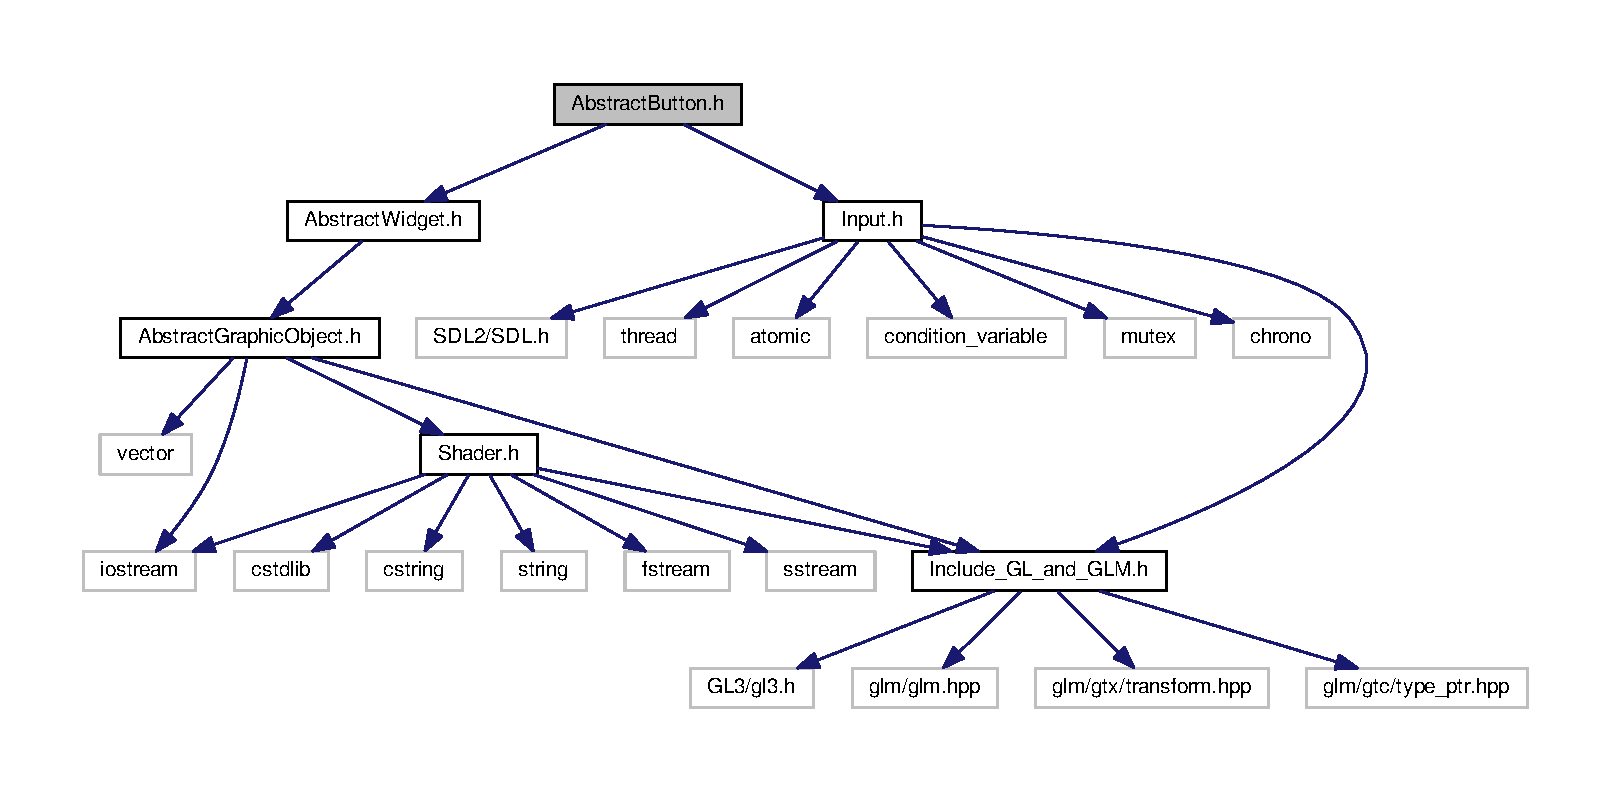
\includegraphics[width=350pt]{AbstractButton_8h__incl}
\end{center}
\end{figure}
\subsection*{Classes}
\begin{DoxyCompactItemize}
\item 
class \hyperlink{classAbstractButton}{Abstract\+Button}
\begin{DoxyCompactList}\small\item\em Type polymorphe pour les boutons. \end{DoxyCompactList}\end{DoxyCompactItemize}


\subsection{Detailed Description}
Définit un type polymorphe pour les boutons. 


\hypertarget{AbstractCamera_8h}{\section{Abstract\-Camera.\-h File Reference}
\label{AbstractCamera_8h}\index{Abstract\-Camera.\-h@{Abstract\-Camera.\-h}}
}


Définit un type polymorphe pour les caméras.  


{\ttfamily \#include \char`\"{}Include\-\_\-\-G\-L\-\_\-and\-\_\-\-G\-L\-M.\-h\char`\"{}}\\*
{\ttfamily \#include \char`\"{}Input.\-h\char`\"{}}\\*
\subsection*{Classes}
\begin{DoxyCompactItemize}
\item 
class \hyperlink{classAbstractCamera}{Abstract\-Camera}
\begin{DoxyCompactList}\small\item\em Type polymorphe pour les caméras (point de vue sur le monde 3\-D) \end{DoxyCompactList}\end{DoxyCompactItemize}


\subsection{Detailed Description}
Définit un type polymorphe pour les caméras. 
\hypertarget{AbstractGraphicObject_8h}{\section{Abstract\+Graphic\+Object.\+h File Reference}
\label{AbstractGraphicObject_8h}\index{Abstract\+Graphic\+Object.\+h@{Abstract\+Graphic\+Object.\+h}}
}


Définit un type polymorphe pour les objets graphiques.  


{\ttfamily \#include $<$iostream$>$}\\*
{\ttfamily \#include $<$vector$>$}\\*
{\ttfamily \#include \char`\"{}Include\+\_\+\+G\+L\+\_\+and\+\_\+\+G\+L\+M.\+h\char`\"{}}\\*
{\ttfamily \#include \char`\"{}Shader.\+h\char`\"{}}\\*
Include dependency graph for Abstract\+Graphic\+Object.\+h\+:\nopagebreak
\begin{figure}[H]
\begin{center}
\leavevmode
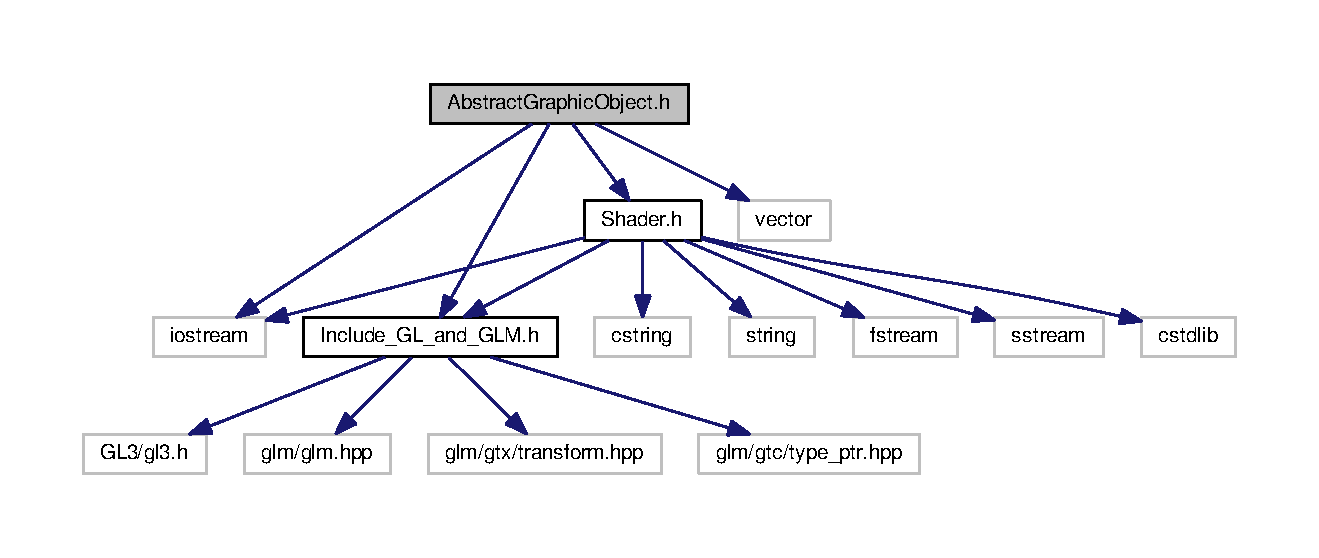
\includegraphics[width=350pt]{AbstractGraphicObject_8h__incl}
\end{center}
\end{figure}
This graph shows which files directly or indirectly include this file\+:\nopagebreak
\begin{figure}[H]
\begin{center}
\leavevmode
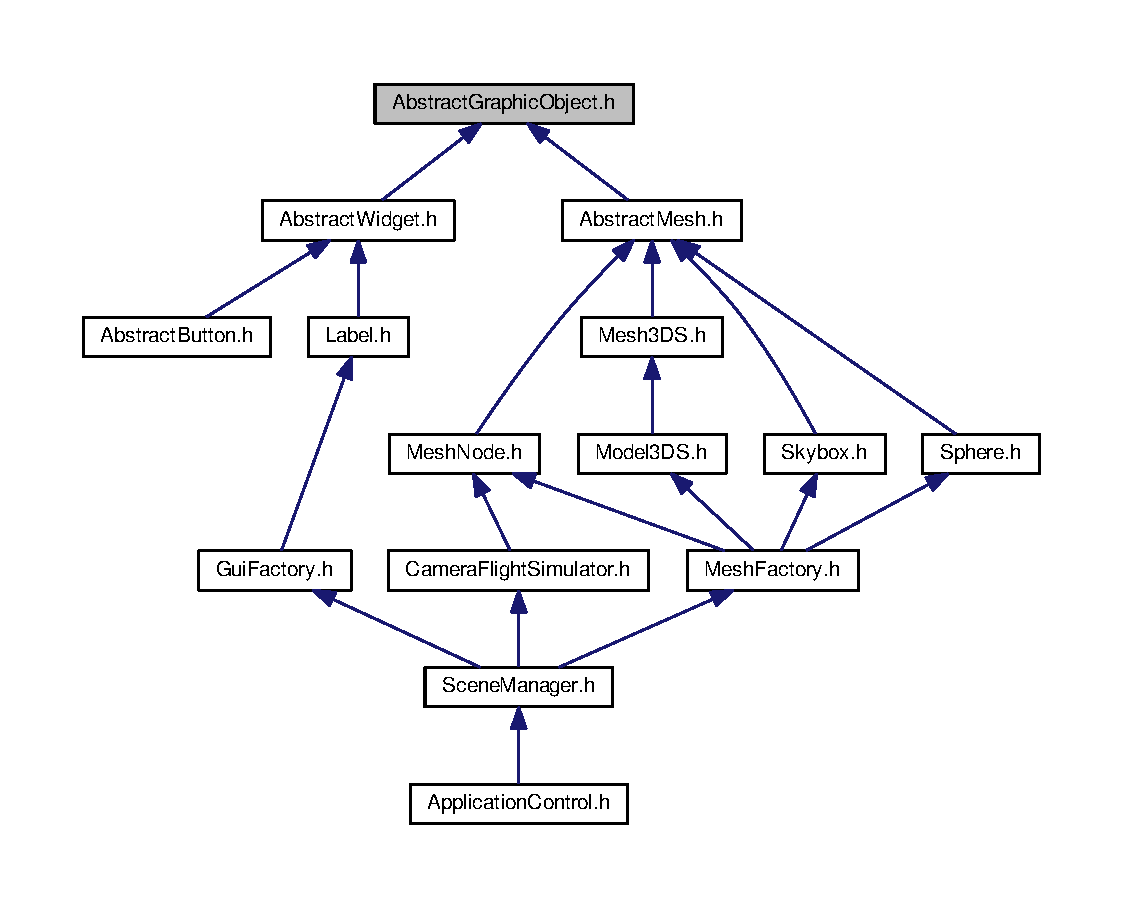
\includegraphics[width=350pt]{AbstractGraphicObject_8h__dep__incl}
\end{center}
\end{figure}
\subsection*{Classes}
\begin{DoxyCompactItemize}
\item 
class \hyperlink{classAbstractGraphicObject}{Abstract\+Graphic\+Object}
\begin{DoxyCompactList}\small\item\em Classe abstraite définissant un type polymorphe pour les objets graphiques. \end{DoxyCompactList}\end{DoxyCompactItemize}
\subsection*{Macros}
\begin{DoxyCompactItemize}
\item 
\hypertarget{AbstractGraphicObject_8h_a2789ab28bb84a9a9f553c45e4eedbdfd}{\#define \hyperlink{AbstractGraphicObject_8h_a2789ab28bb84a9a9f553c45e4eedbdfd}{B\+U\+F\+F\+E\+R\+\_\+\+O\+F\+F\+S\+E\+T}(offset)~((void$\ast$)(offset))}\label{AbstractGraphicObject_8h_a2789ab28bb84a9a9f553c45e4eedbdfd}

\begin{DoxyCompactList}\small\item\em Macro de conversion d'un entier non signé en adresse (utile lors de l'initialisation des vao) \end{DoxyCompactList}\end{DoxyCompactItemize}


\subsection{Detailed Description}
Définit un type polymorphe pour les objets graphiques. 

\begin{DoxyAuthor}{Author}
Raphaël B\+R\+E\+S\+S\+O\+N, Mahdi H\+A\+M\+M\+O\+U\+C\+H\+E 
\end{DoxyAuthor}

\hypertarget{AbstractMesh_8h}{\section{Abstract\-Mesh.\-h File Reference}
\label{AbstractMesh_8h}\index{Abstract\-Mesh.\-h@{Abstract\-Mesh.\-h}}
}


Définition d'un type polymorphe pour les modèles 3\-D.  


{\ttfamily \#include \char`\"{}Abstract\-Graphic\-Object.\-h\char`\"{}}\\*
{\ttfamily \#include \char`\"{}Texture.\-h\char`\"{}}\\*
\subsection*{Classes}
\begin{DoxyCompactItemize}
\item 
class \hyperlink{classAbstractMesh}{Abstract\-Mesh}
\begin{DoxyCompactList}\small\item\em Type polymorphe pour les modèles 3\-D. \end{DoxyCompactList}\end{DoxyCompactItemize}


\subsection{Detailed Description}
Définition d'un type polymorphe pour les modèles 3\-D. 
\hypertarget{AbstractWidget_8h}{\section{Abstract\-Widget.\-h File Reference}
\label{AbstractWidget_8h}\index{Abstract\-Widget.\-h@{Abstract\-Widget.\-h}}
}


Définit un type polymorphe pour les objets 2\-D.  


{\ttfamily \#include \char`\"{}Abstract\-Graphic\-Object.\-h\char`\"{}}\\*
\subsection*{Classes}
\begin{DoxyCompactItemize}
\item 
class \hyperlink{classAbstractWidget}{Abstract\-Widget}
\begin{DoxyCompactList}\small\item\em Classe abstraite mère de tous les objets 2\-D. \end{DoxyCompactList}\end{DoxyCompactItemize}


\subsection{Detailed Description}
Définit un type polymorphe pour les objets 2\-D. 
\hypertarget{ApplicationControl_8h}{\section{Application\-Control.\-h File Reference}
\label{ApplicationControl_8h}\index{Application\-Control.\-h@{Application\-Control.\-h}}
}


Gestion de la S\-D\-L et de Open\-G\-L ainsi que du \hyperlink{classSceneManager}{Scene\-Manager}.  


{\ttfamily \#include $<$iostream$>$}\\*
{\ttfamily \#include $<$string$>$}\\*
{\ttfamily \#include $<$S\-D\-L2/\-S\-D\-L.\-h$>$}\\*
{\ttfamily \#include $<$S\-D\-L2/\-S\-D\-L\-\_\-image.\-h$>$}\\*
{\ttfamily \#include $<$S\-D\-L2/\-S\-D\-L\-\_\-ttf.\-h$>$}\\*
{\ttfamily \#include $<$S\-D\-L2/\-S\-D\-L\-\_\-mixer.\-h$>$}\\*
{\ttfamily \#include \char`\"{}Include\-\_\-\-G\-L\-\_\-and\-\_\-\-G\-L\-M.\-h\char`\"{}}\\*
{\ttfamily \#include \char`\"{}Input.\-h\char`\"{}}\\*
{\ttfamily \#include \char`\"{}Scene\-Manager.\-h\char`\"{}}\\*
\subsection*{Classes}
\begin{DoxyCompactItemize}
\item 
class \hyperlink{classApplicationControl}{Application\-Control}
\begin{DoxyCompactList}\small\item\em Classe repésentant globalement le programme graphique. \end{DoxyCompactList}\end{DoxyCompactItemize}


\subsection{Detailed Description}
Gestion de la S\-D\-L et de Open\-G\-L ainsi que du \hyperlink{classSceneManager}{Scene\-Manager}. \begin{DoxyAuthor}{Author}
Raphaël B\-R\-E\-S\-S\-O\-N, Mahdi H\-A\-M\-M\-O\-U\-C\-H\-E 
\end{DoxyAuthor}

\hypertarget{CameraFlightSimulator_8h}{\section{Camera\-Flight\-Simulator.\-h File Reference}
\label{CameraFlightSimulator_8h}\index{Camera\-Flight\-Simulator.\-h@{Camera\-Flight\-Simulator.\-h}}
}


Implémentation de la caméra de simulateur de vol.  


{\ttfamily \#include \char`\"{}Abstract\-Camera.\-h\char`\"{}}\\*
{\ttfamily \#include \char`\"{}Mesh\-Node.\-h\char`\"{}}\\*
\subsection*{Classes}
\begin{DoxyCompactItemize}
\item 
class \hyperlink{classCameraFlightSimulator}{Camera\-Flight\-Simulator}
\begin{DoxyCompactList}\small\item\em Implémentation de la caméra de simulateur de vol. \end{DoxyCompactList}\end{DoxyCompactItemize}


\subsection{Detailed Description}
Implémentation de la caméra de simulateur de vol. 
\hypertarget{CameraFPS_8h}{\section{Camera\+F\+P\+S.\+h File Reference}
\label{CameraFPS_8h}\index{Camera\+F\+P\+S.\+h@{Camera\+F\+P\+S.\+h}}
}


Définition de la caméra à la première personne.  


{\ttfamily \#include \char`\"{}Abstract\+Camera.\+h\char`\"{}}\\*
Include dependency graph for Camera\+F\+P\+S.\+h\+:
\nopagebreak
\begin{figure}[H]
\begin{center}
\leavevmode
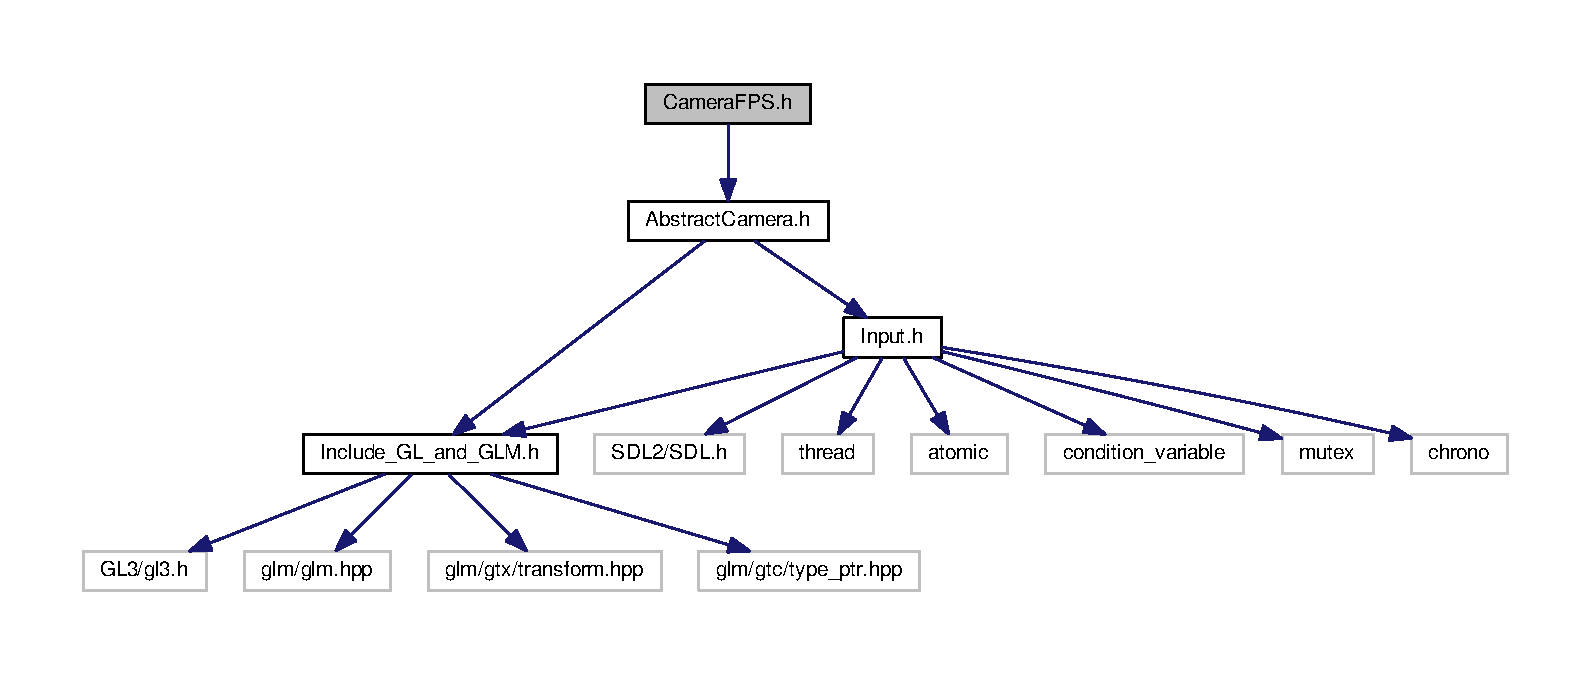
\includegraphics[width=350pt]{CameraFPS_8h__incl}
\end{center}
\end{figure}
This graph shows which files directly or indirectly include this file\+:\nopagebreak
\begin{figure}[H]
\begin{center}
\leavevmode
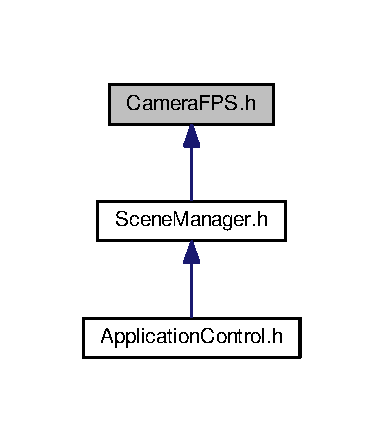
\includegraphics[width=184pt]{CameraFPS_8h__dep__incl}
\end{center}
\end{figure}
\subsection*{Classes}
\begin{DoxyCompactItemize}
\item 
class \hyperlink{classCameraFPS}{Camera\+F\+P\+S}
\begin{DoxyCompactList}\small\item\em Caméra de type Freefly à deux degrés de liberté en fixant l'axe vertical. \end{DoxyCompactList}\end{DoxyCompactItemize}


\subsection{Detailed Description}
Définition de la caméra à la première personne. 


\hypertarget{Font_8h}{\section{Font.\-h File Reference}
\label{Font_8h}\index{Font.\-h@{Font.\-h}}
}


Gestion de la génération de texte.  


{\ttfamily \#include \char`\"{}Texture.\-h\char`\"{}}\\*
\subsection*{Classes}
\begin{DoxyCompactItemize}
\item 
class \hyperlink{classFont}{Font}
\begin{DoxyCompactList}\small\item\em Gère la conversion de texte en texture G\-L à partir d'une police. \end{DoxyCompactList}\end{DoxyCompactItemize}


\subsection{Detailed Description}
Gestion de la génération de texte. \begin{DoxyAuthor}{Author}
Raphaël B\-R\-E\-S\-S\-O\-N, Mehdi H\-A\-M\-M\-O\-U\-C\-H\-E 
\end{DoxyAuthor}

\hypertarget{GuiFactory_8h}{\section{Gui\-Factory.\-h File Reference}
\label{GuiFactory_8h}\index{Gui\-Factory.\-h@{Gui\-Factory.\-h}}
}


Gestion de la construction des objets 2\-D.  


{\ttfamily \#include \char`\"{}Label.\-h\char`\"{}}\\*
\subsection*{Classes}
\begin{DoxyCompactItemize}
\item 
class \hyperlink{classGuiFactory}{Gui\-Factory}
\begin{DoxyCompactList}\small\item\em Classe de création d'objets 2\-D \-: contient les shaders d'affichage 2\-D. \end{DoxyCompactList}\end{DoxyCompactItemize}
\subsection*{Macros}
\begin{DoxyCompactItemize}
\item 
\hypertarget{GuiFactory_8h_ab95fd09ba03ef5f9fd678105ee906e42}{\#define \hyperlink{GuiFactory_8h_ab95fd09ba03ef5f9fd678105ee906e42}{V\-E\-R\-T\-E\-X\-\_\-\-S\-H\-A\-D\-E\-R\-\_\-\-G\-U\-I}~\char`\"{}Shaders/shader\-Gui.\-vert\char`\"{}}\label{GuiFactory_8h_ab95fd09ba03ef5f9fd678105ee906e42}

\begin{DoxyCompactList}\small\item\em Vertex shader pour un objet 2\-D. \end{DoxyCompactList}\item 
\hypertarget{GuiFactory_8h_a8659ace818b251e3dbd0dbe51bc8c872}{\#define \hyperlink{GuiFactory_8h_a8659ace818b251e3dbd0dbe51bc8c872}{F\-R\-A\-G\-M\-E\-N\-T\-\_\-\-S\-H\-A\-D\-E\-R\-\_\-\-G\-U\-I\-\_\-\-T\-E\-X\-T\-U\-R\-E}~\char`\"{}Shaders/shader\-Gui\-Texture.\-frag\char`\"{}}\label{GuiFactory_8h_a8659ace818b251e3dbd0dbe51bc8c872}

\begin{DoxyCompactList}\small\item\em Fragment shader pour un objet texturé \end{DoxyCompactList}\item 
\hypertarget{GuiFactory_8h_a1bb33c88727317de93ebd205aa334381}{\#define \hyperlink{GuiFactory_8h_a1bb33c88727317de93ebd205aa334381}{F\-R\-A\-G\-M\-E\-N\-T\-\_\-\-S\-H\-A\-D\-E\-R\-\_\-\-G\-U\-I\-\_\-\-C\-O\-L\-O\-R}~\char`\"{}Shaders/gui\-Color.\-vert\char`\"{}}\label{GuiFactory_8h_a1bb33c88727317de93ebd205aa334381}

\begin{DoxyCompactList}\small\item\em Fragment shader pour un objet non texturé (coloré) \end{DoxyCompactList}\item 
\hypertarget{GuiFactory_8h_adc8de613e03fa6154949c39666d33ded}{\#define \hyperlink{GuiFactory_8h_adc8de613e03fa6154949c39666d33ded}{F\-O\-N\-T\-\_\-7\-S\-E\-G\-M\-E\-N\-T}~\char`\"{}Fonts/7seg.\-ttf\char`\"{}}\label{GuiFactory_8h_adc8de613e03fa6154949c39666d33ded}

\begin{DoxyCompactList}\small\item\em Fichier de la police \char`\"{}afficheur 7 segments\char`\"{}. \end{DoxyCompactList}\item 
\hypertarget{GuiFactory_8h_ae544f02e3ffcee0404f27578a577b97b}{\#define \hyperlink{GuiFactory_8h_ae544f02e3ffcee0404f27578a577b97b}{F\-O\-N\-T\-\_\-\-C\-O\-U\-N\-T\-E\-R\-\_\-\-S\-T\-R\-I\-K\-E}~\char`\"{}Fonts/cs.\-ttf\char`\"{}}\label{GuiFactory_8h_ae544f02e3ffcee0404f27578a577b97b}

\begin{DoxyCompactList}\small\item\em Fichier de la police du jeu Counter Strike. \end{DoxyCompactList}\item 
\hypertarget{GuiFactory_8h_acde9ec8712f62632c6a8fcacfe6800c4}{\#define \hyperlink{GuiFactory_8h_acde9ec8712f62632c6a8fcacfe6800c4}{D\-E\-F\-A\-U\-L\-T\-\_\-\-F\-O\-N\-T\-\_\-\-S\-I\-Z\-E}~50}\label{GuiFactory_8h_acde9ec8712f62632c6a8fcacfe6800c4}

\begin{DoxyCompactList}\small\item\em Taille par défault (résolution verticale) du texte affiché à l'écran. \end{DoxyCompactList}\end{DoxyCompactItemize}


\subsection{Detailed Description}
Gestion de la construction des objets 2\-D. \begin{DoxyAuthor}{Author}
Raphaël B\-R\-E\-S\-S\-O\-N, Mahdi H\-A\-M\-M\-O\-U\-C\-H\-E 
\end{DoxyAuthor}

\hypertarget{Include__GL__and__GLM_8h}{\section{Include\+\_\+\+G\+L\+\_\+and\+\_\+\+G\+L\+M.\+h File Reference}
\label{Include__GL__and__GLM_8h}\index{Include\+\_\+\+G\+L\+\_\+and\+\_\+\+G\+L\+M.\+h@{Include\+\_\+\+G\+L\+\_\+and\+\_\+\+G\+L\+M.\+h}}
}


Inclusion des header de Open\+G\+L 3 et G\+L\+M.  


{\ttfamily \#include $<$G\+L3/gl3.\+h$>$}\\*
{\ttfamily \#include $<$glm/glm.\+hpp$>$}\\*
{\ttfamily \#include $<$glm/gtx/transform.\+hpp$>$}\\*
{\ttfamily \#include $<$glm/gtc/type\+\_\+ptr.\+hpp$>$}\\*
Include dependency graph for Include\+\_\+\+G\+L\+\_\+and\+\_\+\+G\+L\+M.\+h\+:\nopagebreak
\begin{figure}[H]
\begin{center}
\leavevmode
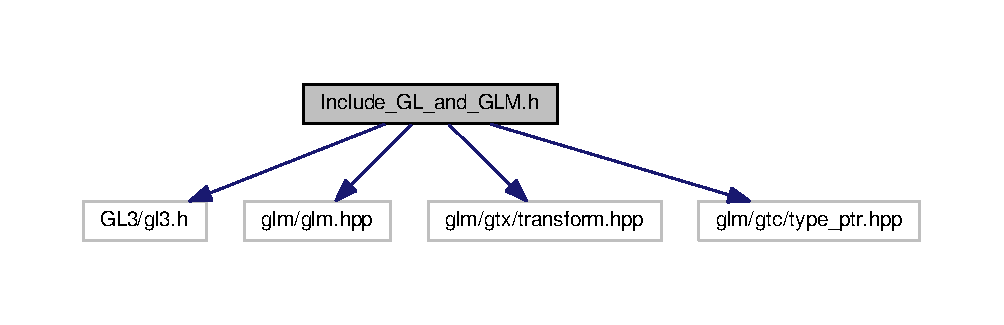
\includegraphics[width=350pt]{Include__GL__and__GLM_8h__incl}
\end{center}
\end{figure}
This graph shows which files directly or indirectly include this file\+:
\nopagebreak
\begin{figure}[H]
\begin{center}
\leavevmode
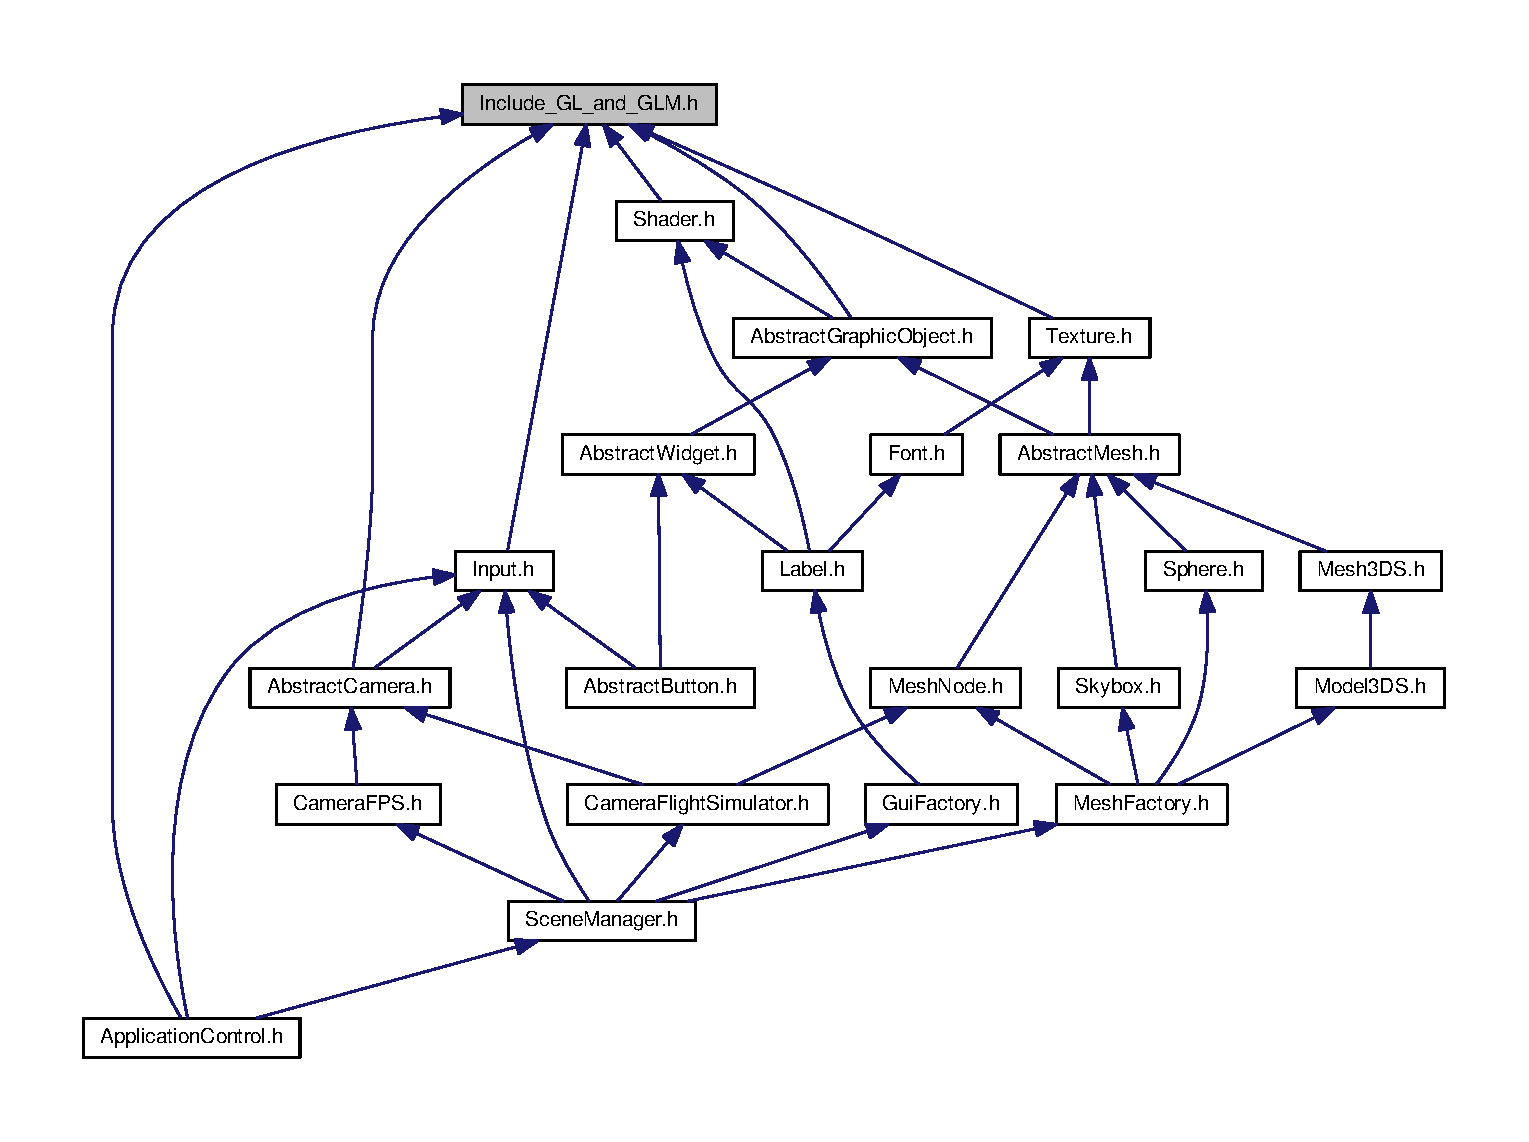
\includegraphics[width=350pt]{Include__GL__and__GLM_8h__dep__incl}
\end{center}
\end{figure}
\subsection*{Macros}
\begin{DoxyCompactItemize}
\item 
\hypertarget{Include__GL__and__GLM_8h_a513ae87770898727d346eced6be03bdd}{\#define \hyperlink{Include__GL__and__GLM_8h_a513ae87770898727d346eced6be03bdd}{G\+L3\+\_\+\+P\+R\+O\+T\+O\+T\+Y\+P\+E\+S}~1}\label{Include__GL__and__GLM_8h_a513ae87770898727d346eced6be03bdd}

\begin{DoxyCompactList}\small\item\em Obligatoire sur Linux et Mac O\+S (forcer à 1) \end{DoxyCompactList}\end{DoxyCompactItemize}


\subsection{Detailed Description}
Inclusion des header de Open\+G\+L 3 et G\+L\+M. 

\begin{DoxyAuthor}{Author}
Raphaël B\+R\+E\+S\+S\+O\+N, Mahdi H\+A\+M\+M\+O\+U\+C\+H\+E 
\end{DoxyAuthor}

\hypertarget{Input_8h}{\section{Input.\+h File Reference}
\label{Input_8h}\index{Input.\+h@{Input.\+h}}
}
{\ttfamily \#include \char`\"{}Include\+\_\+\+G\+L\+\_\+and\+\_\+\+G\+L\+M.\+h\char`\"{}}\\*
{\ttfamily \#include $<$S\+D\+L2/\+S\+D\+L.\+h$>$}\\*
{\ttfamily \#include $<$thread$>$}\\*
{\ttfamily \#include $<$atomic$>$}\\*
{\ttfamily \#include $<$condition\+\_\+variable$>$}\\*
{\ttfamily \#include $<$mutex$>$}\\*
{\ttfamily \#include $<$chrono$>$}\\*
Include dependency graph for Input.\+h\+:
\nopagebreak
\begin{figure}[H]
\begin{center}
\leavevmode
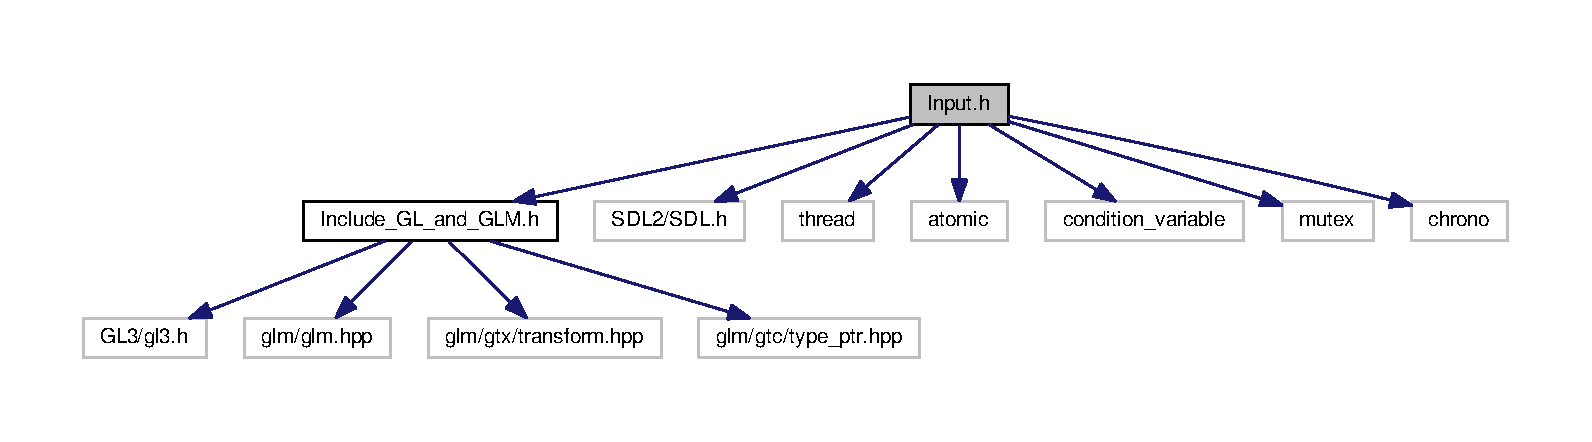
\includegraphics[width=350pt]{Input_8h__incl}
\end{center}
\end{figure}
This graph shows which files directly or indirectly include this file\+:
\nopagebreak
\begin{figure}[H]
\begin{center}
\leavevmode
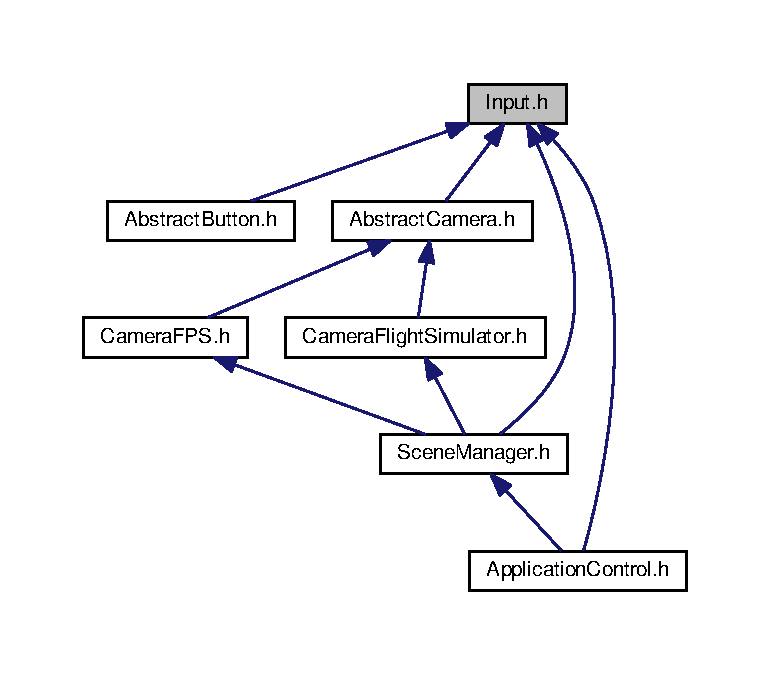
\includegraphics[width=350pt]{Input_8h__dep__incl}
\end{center}
\end{figure}
\subsection*{Classes}
\begin{DoxyCompactItemize}
\item 
class \hyperlink{classInput}{Input}
\begin{DoxyCompactList}\small\item\em gestion des évênements \end{DoxyCompactList}\end{DoxyCompactItemize}


\subsection{Detailed Description}
\begin{DoxyAuthor}{Authors}
Raphaël B\+R\+E\+S\+S\+O\+N, Mehdi H\+A\+M\+M\+O\+U\+C\+H\+E 
\end{DoxyAuthor}

\hypertarget{Label_8h}{\section{Label.\-h File Reference}
\label{Label_8h}\index{Label.\-h@{Label.\-h}}
}


Gestion de l'affichage de texte.  


{\ttfamily \#include \char`\"{}Font.\-h\char`\"{}}\\*
{\ttfamily \#include \char`\"{}Shader.\-h\char`\"{}}\\*
{\ttfamily \#include \char`\"{}Abstract\-Widget.\-h\char`\"{}}\\*
\subsection*{Classes}
\begin{DoxyCompactItemize}
\item 
class \hyperlink{classLabel}{Label}
\begin{DoxyCompactList}\small\item\em Représente un objet Texte 2\-D. \end{DoxyCompactList}\end{DoxyCompactItemize}


\subsection{Detailed Description}
Gestion de l'affichage de texte. \begin{DoxyAuthor}{Author}
Raphaël B\-R\-E\-S\-S\-O\-N, Mahdi H\-A\-M\-M\-O\-U\-C\-H\-E 
\end{DoxyAuthor}

\hypertarget{Mesh3DS_8h}{\section{Mesh3\-D\-S.\-h File Reference}
\label{Mesh3DS_8h}\index{Mesh3\-D\-S.\-h@{Mesh3\-D\-S.\-h}}
}


Définition d'un mesh d'un modèle 3\-D\-S.  


{\ttfamily \#include \char`\"{}Abstract\-Mesh.\-h\char`\"{}}\\*
{\ttfamily \#include $<$lib3ds/file.\-h$>$}\\*
{\ttfamily \#include $<$lib3ds/node.\-h$>$}\\*
{\ttfamily \#include $<$lib3ds/mesh.\-h$>$}\\*
{\ttfamily \#include $<$lib3ds/vector.\-h$>$}\\*
{\ttfamily \#include $<$lib3ds/matrix.\-h$>$}\\*
{\ttfamily \#include $<$lib3ds/material.\-h$>$}\\*
\subsection*{Classes}
\begin{DoxyCompactItemize}
\item 
class \hyperlink{classMesh3DS}{Mesh3\-D\-S}
\begin{DoxyCompactList}\small\item\em Mesh d'un modèle 3\-D\-S. \end{DoxyCompactList}\end{DoxyCompactItemize}


\subsection{Detailed Description}
Définition d'un mesh d'un modèle 3\-D\-S. 
\hypertarget{MeshFactory_8h}{\section{Mesh\-Factory.\-h File Reference}
\label{MeshFactory_8h}\index{Mesh\-Factory.\-h@{Mesh\-Factory.\-h}}
}


Construction d'objets 3\-D et gestion des shaders.  


{\ttfamily \#include \char`\"{}Mesh\-Node.\-h\char`\"{}}\\*
{\ttfamily \#include \char`\"{}Model3\-D\-S.\-h\char`\"{}}\\*
{\ttfamily \#include \char`\"{}Skybox.\-h\char`\"{}}\\*
{\ttfamily \#include \char`\"{}Sphere.\-h\char`\"{}}\\*
{\ttfamily \#include $<$map$>$}\\*
\subsection*{Classes}
\begin{DoxyCompactItemize}
\item 
class \hyperlink{classMeshFactory}{Mesh\-Factory}
\begin{DoxyCompactList}\small\item\em Classe de gestion des shaders et de génération des modèles 3\-D. \end{DoxyCompactList}\end{DoxyCompactItemize}
\subsection*{Macros}
\begin{DoxyCompactItemize}
\item 
\hypertarget{MeshFactory_8h_a0c7dd92a18d7046d3b50e7e80cf5f90f}{\#define \hyperlink{MeshFactory_8h_a0c7dd92a18d7046d3b50e7e80cf5f90f}{V\-E\-R\-T\-E\-X\-\_\-\-S\-H\-A\-D\-E\-R\-\_\-3\-D}~\char`\"{}Shaders/shader3\-D.\-vert\char`\"{}}\label{MeshFactory_8h_a0c7dd92a18d7046d3b50e7e80cf5f90f}

\begin{DoxyCompactList}\small\item\em Nom du vertex shader pour l'affichage 3\-D. \end{DoxyCompactList}\item 
\hypertarget{MeshFactory_8h_abb985244f0bf98badef6e8ecdc57bcf9}{\#define \hyperlink{MeshFactory_8h_abb985244f0bf98badef6e8ecdc57bcf9}{F\-R\-A\-G\-M\-E\-N\-T\-\_\-\-S\-H\-A\-D\-E\-R\-\_\-3\-D\-\_\-\-T\-E\-X\-T\-U\-R\-E\-\_\-2\-D}~\char`\"{}Shaders/shader3\-D\-Texture2\-D.\-frag\char`\"{}}\label{MeshFactory_8h_abb985244f0bf98badef6e8ecdc57bcf9}

\begin{DoxyCompactList}\small\item\em Nom du fragment shader pour l'affichage 3\-D avec une texture 2\-D. \end{DoxyCompactList}\end{DoxyCompactItemize}


\subsection{Detailed Description}
Construction d'objets 3\-D et gestion des shaders. 
\hypertarget{MeshNode_8h}{\section{Mesh\-Node.\-h File Reference}
\label{MeshNode_8h}\index{Mesh\-Node.\-h@{Mesh\-Node.\-h}}
}


Définition de la classe de gestion de modèles 3\-D.  


{\ttfamily \#include \char`\"{}Abstract\-Mesh.\-h\char`\"{}}\\*
\subsection*{Classes}
\begin{DoxyCompactItemize}
\item 
class \hyperlink{classMeshNode}{Mesh\-Node}
\begin{DoxyCompactList}\small\item\em Classe de gestion de modèles 3\-D. \end{DoxyCompactList}\end{DoxyCompactItemize}


\subsection{Detailed Description}
Définition de la classe de gestion de modèles 3\-D. 
\hypertarget{Model3DS_8h}{\section{Model3\+D\+S.\+h File Reference}
\label{Model3DS_8h}\index{Model3\+D\+S.\+h@{Model3\+D\+S.\+h}}
}


Importation d'un modèle 3\+D depuis le format 3\+D\+S M\+A\+X (sans les animations)  


{\ttfamily \#include \char`\"{}Mesh3\+D\+S.\+h\char`\"{}}\\*
Include dependency graph for Model3\+D\+S.\+h\+:\nopagebreak
\begin{figure}[H]
\begin{center}
\leavevmode
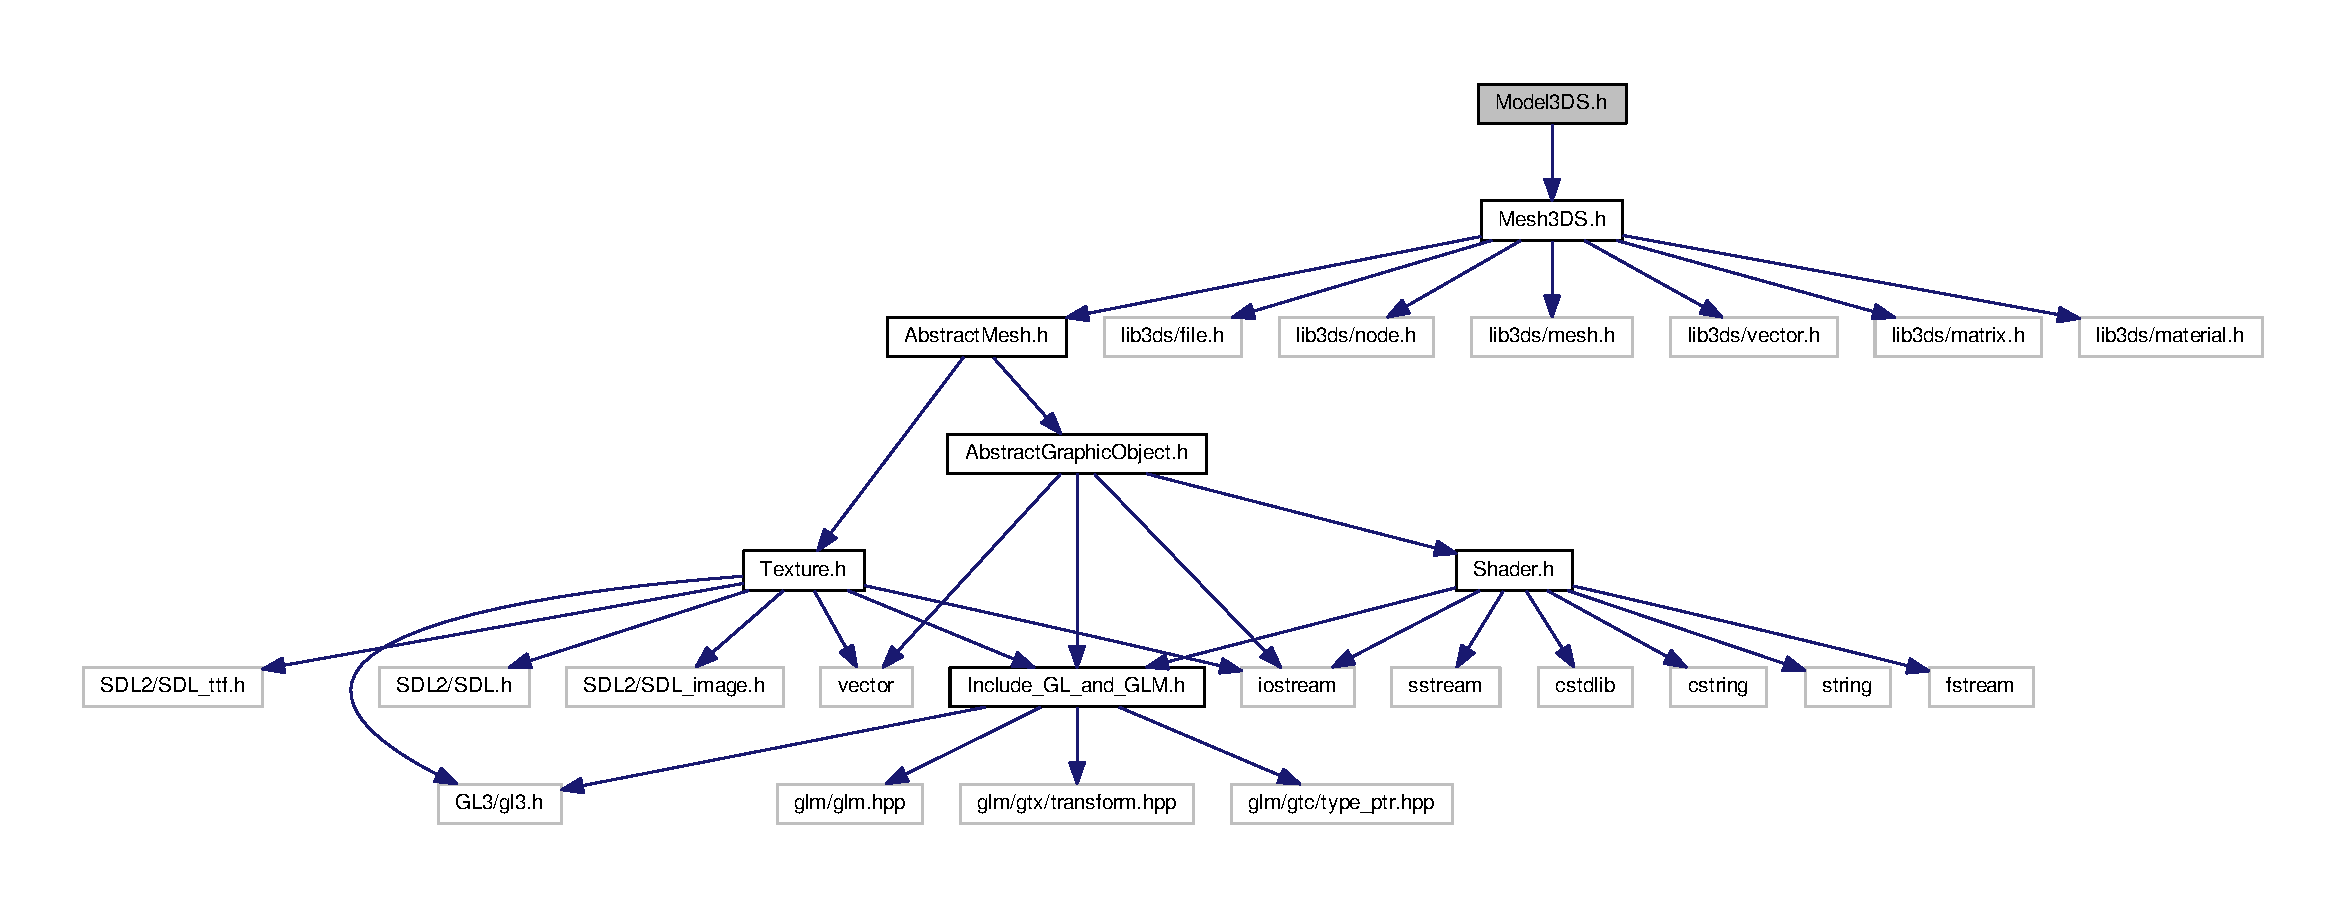
\includegraphics[width=350pt]{Model3DS_8h__incl}
\end{center}
\end{figure}
This graph shows which files directly or indirectly include this file\+:\nopagebreak
\begin{figure}[H]
\begin{center}
\leavevmode
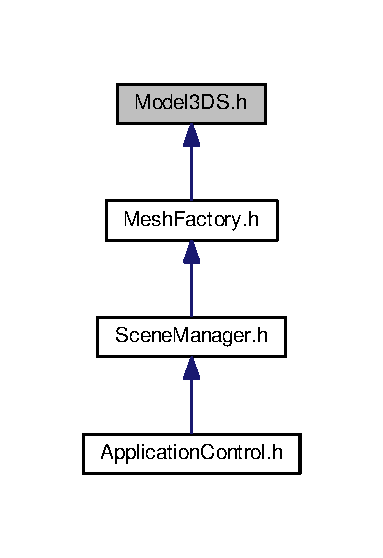
\includegraphics[width=184pt]{Model3DS_8h__dep__incl}
\end{center}
\end{figure}
\subsection*{Classes}
\begin{DoxyCompactItemize}
\item 
class \hyperlink{classModel3DS}{Model3\+D\+S}
\begin{DoxyCompactList}\small\item\em Gestion des modèle 3\+D\+S. \end{DoxyCompactList}\end{DoxyCompactItemize}


\subsection{Detailed Description}
Importation d'un modèle 3\+D depuis le format 3\+D\+S M\+A\+X (sans les animations) 


\hypertarget{SceneManager_8h}{\section{Scene\+Manager.\+h File Reference}
\label{SceneManager_8h}\index{Scene\+Manager.\+h@{Scene\+Manager.\+h}}
}


Gestion des modèles et de l'affichage.  


{\ttfamily \#include $<$iostream$>$}\\*
{\ttfamily \#include $<$vector$>$}\\*
{\ttfamily \#include $<$string$>$}\\*
{\ttfamily \#include \char`\"{}Camera\+F\+P\+S.\+h\char`\"{}}\\*
{\ttfamily \#include \char`\"{}Camera\+Flight\+Simulator.\+h\char`\"{}}\\*
{\ttfamily \#include \char`\"{}Input.\+h\char`\"{}}\\*
{\ttfamily \#include \char`\"{}Mesh\+Factory.\+h\char`\"{}}\\*
{\ttfamily \#include \char`\"{}Gui\+Factory.\+h\char`\"{}}\\*
{\ttfamily \#include \char`\"{}Sound\+Manager.\+h\char`\"{}}\\*
Include dependency graph for Scene\+Manager.\+h\+:
\nopagebreak
\begin{figure}[H]
\begin{center}
\leavevmode
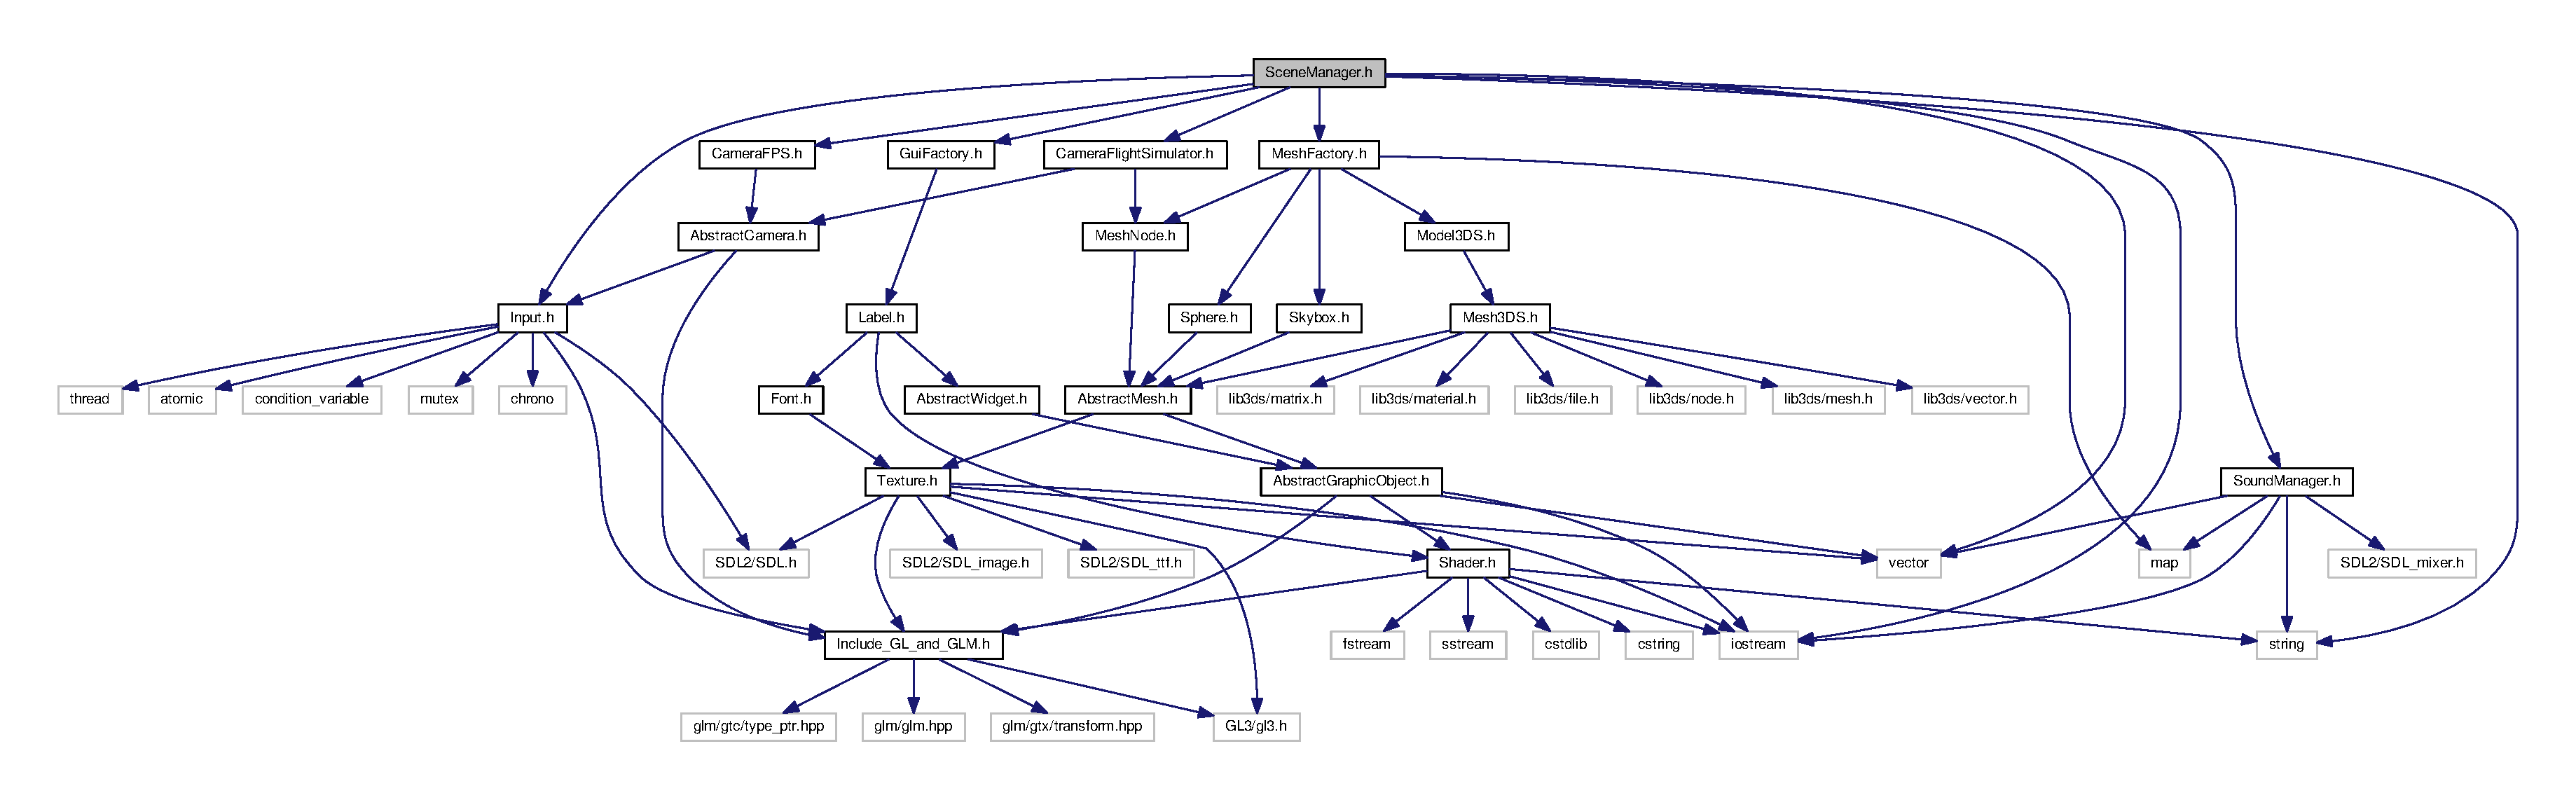
\includegraphics[width=350pt]{SceneManager_8h__incl}
\end{center}
\end{figure}
This graph shows which files directly or indirectly include this file\+:\nopagebreak
\begin{figure}[H]
\begin{center}
\leavevmode
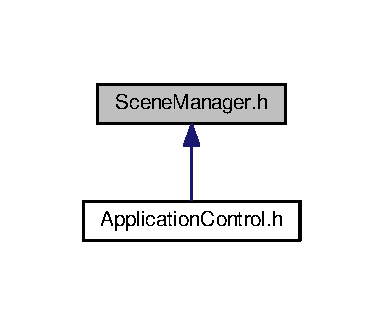
\includegraphics[width=184pt]{SceneManager_8h__dep__incl}
\end{center}
\end{figure}
\subsection*{Classes}
\begin{DoxyCompactItemize}
\item 
class \hyperlink{classSceneManager}{Scene\+Manager}
\begin{DoxyCompactList}\small\item\em Gestionnaire des modèle, des caméras (pour le 3\+D) et de l'affichage. \end{DoxyCompactList}\end{DoxyCompactItemize}
\subsection*{Macros}
\begin{DoxyCompactItemize}
\item 
\hypertarget{SceneManager_8h_a69c339b2966791489487938c49401cf3}{\#define \hyperlink{SceneManager_8h_a69c339b2966791489487938c49401cf3}{F\+P\+S\+\_\+\+L\+I\+M\+I\+T}~60}\label{SceneManager_8h_a69c339b2966791489487938c49401cf3}

\begin{DoxyCompactList}\small\item\em Limitation de la fréquence de rafraichissement à 60 F\+P\+S. \end{DoxyCompactList}\end{DoxyCompactItemize}


\subsection{Detailed Description}
Gestion des modèles et de l'affichage. 

Raphaël B\+R\+E\+S\+S\+O\+N, Mahdi H\+A\+M\+M\+O\+U\+C\+H\+E 
\hypertarget{Shader_8h}{\section{Shader.\+h File Reference}
\label{Shader_8h}\index{Shader.\+h@{Shader.\+h}}
}


Gestion des Shaders (Programmes pour le G\+P\+U)  


{\ttfamily \#include \char`\"{}Include\+\_\+\+G\+L\+\_\+and\+\_\+\+G\+L\+M.\+h\char`\"{}}\\*
{\ttfamily \#include $<$iostream$>$}\\*
{\ttfamily \#include $<$cstdlib$>$}\\*
{\ttfamily \#include $<$cstring$>$}\\*
{\ttfamily \#include $<$string$>$}\\*
{\ttfamily \#include $<$fstream$>$}\\*
{\ttfamily \#include $<$sstream$>$}\\*
Include dependency graph for Shader.\+h\+:\nopagebreak
\begin{figure}[H]
\begin{center}
\leavevmode
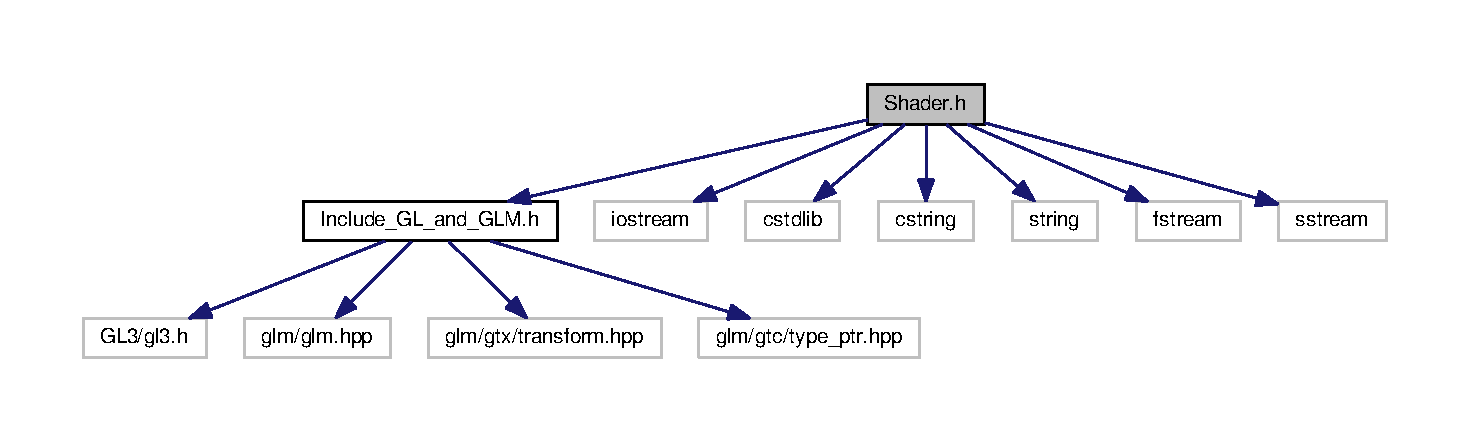
\includegraphics[width=350pt]{Shader_8h__incl}
\end{center}
\end{figure}
This graph shows which files directly or indirectly include this file\+:\nopagebreak
\begin{figure}[H]
\begin{center}
\leavevmode
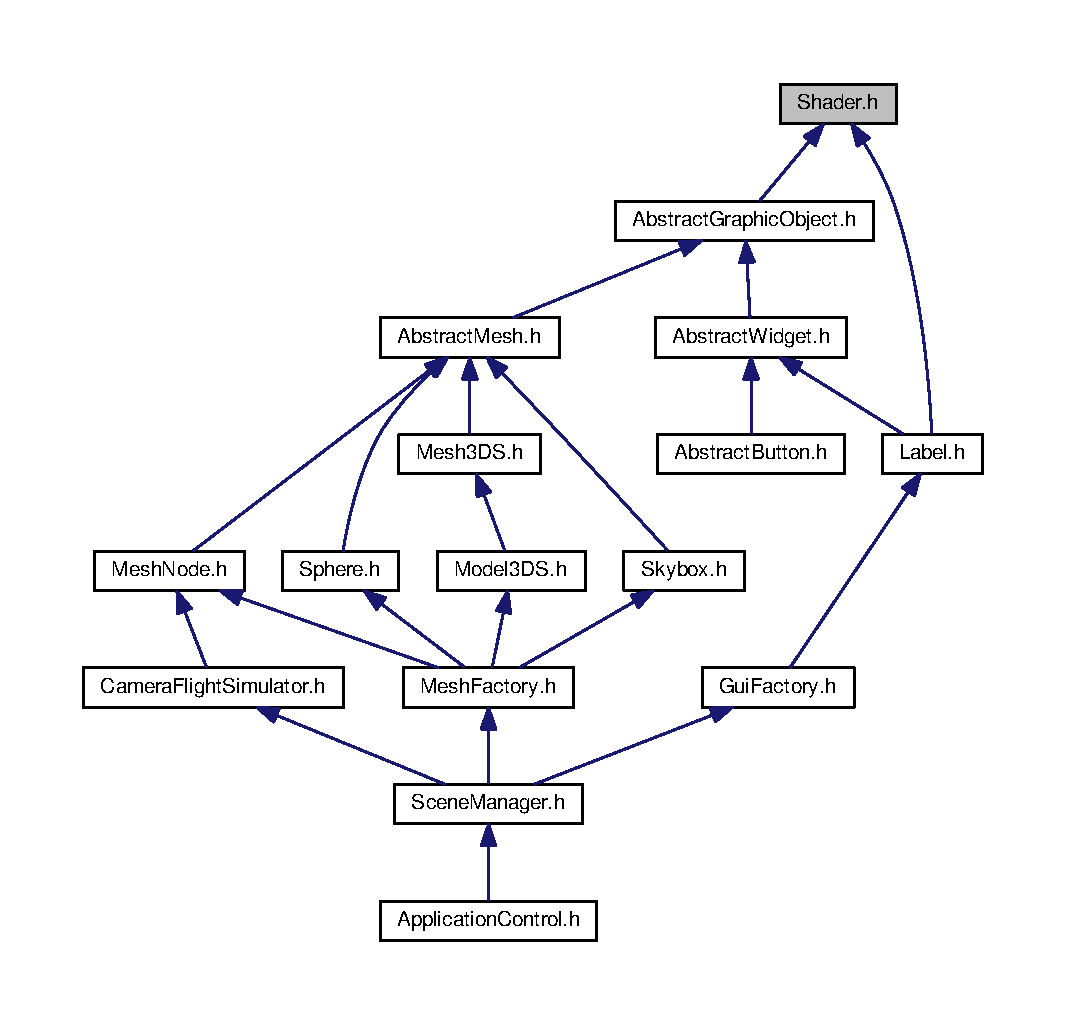
\includegraphics[width=350pt]{Shader_8h__dep__incl}
\end{center}
\end{figure}
\subsection*{Classes}
\begin{DoxyCompactItemize}
\item 
class \hyperlink{classShader}{Shader}
\begin{DoxyCompactList}\small\item\em Classe de gestion de programmes shaders (compilation, édition de liens, contrôle et destruction) \end{DoxyCompactList}\end{DoxyCompactItemize}


\subsection{Detailed Description}
Gestion des Shaders (Programmes pour le G\+P\+U) 


\hypertarget{Skybox_8h}{\section{Skybox.\+h File Reference}
\label{Skybox_8h}\index{Skybox.\+h@{Skybox.\+h}}
}


Simulation d'environnement via skybox monotexturée.  


{\ttfamily \#include \char`\"{}Abstract\+Mesh.\+h\char`\"{}}\\*
Include dependency graph for Skybox.\+h\+:\nopagebreak
\begin{figure}[H]
\begin{center}
\leavevmode
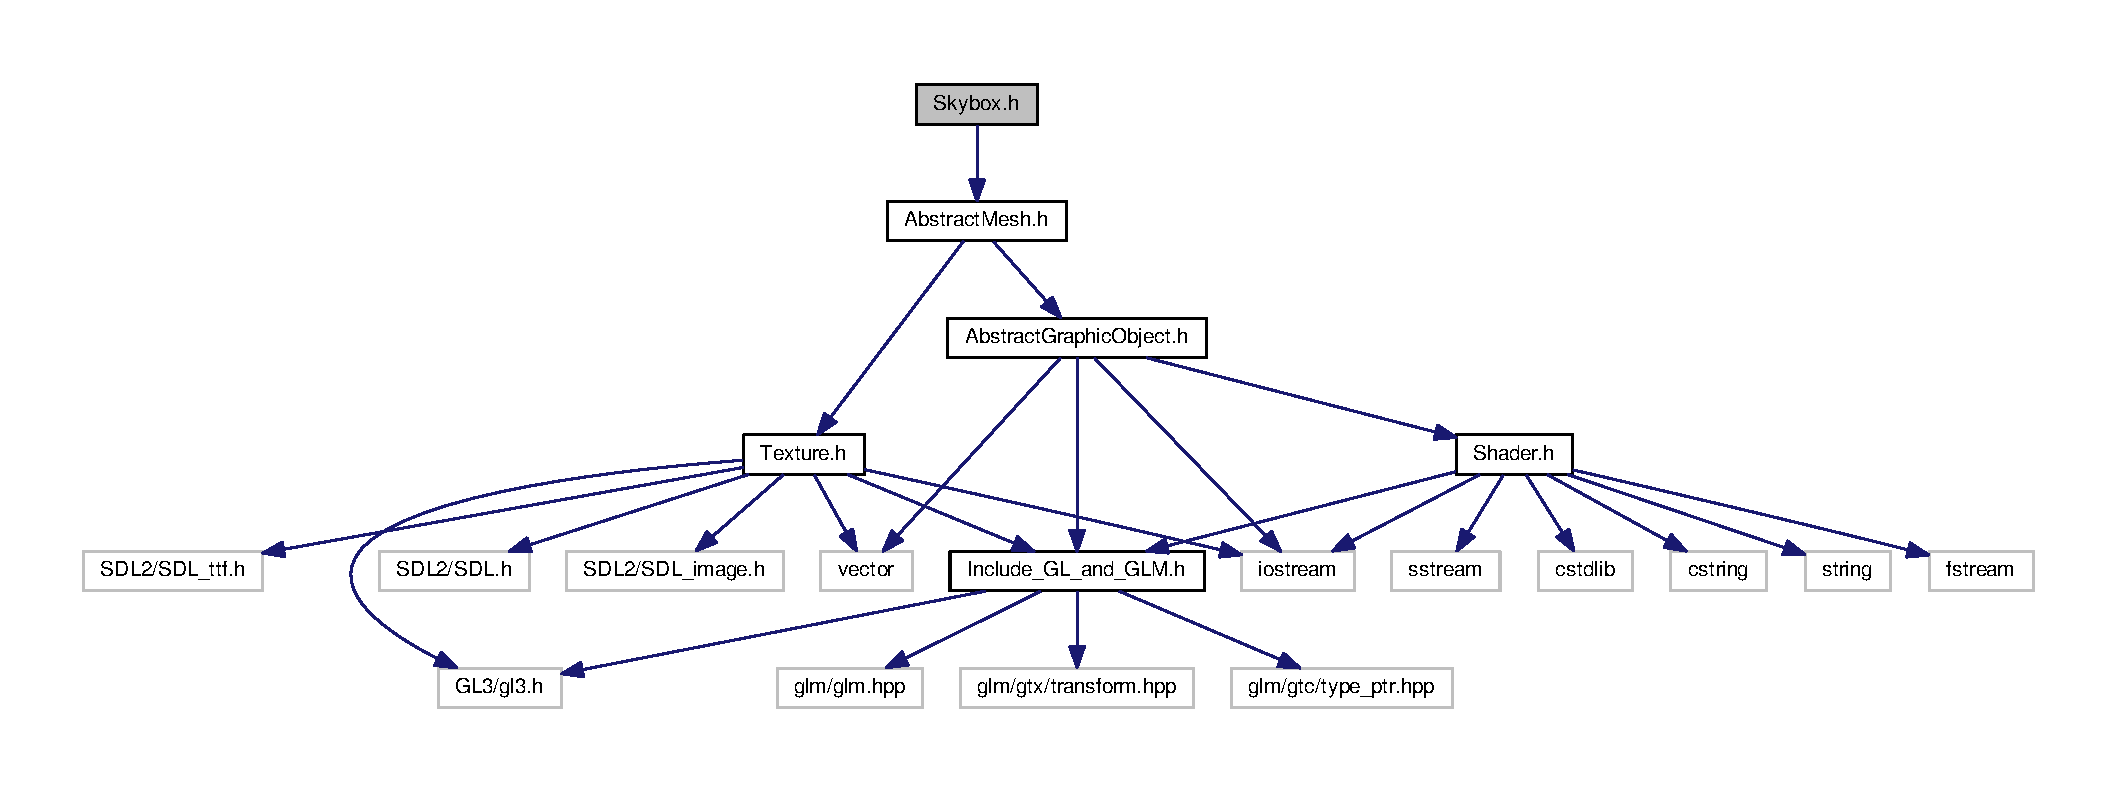
\includegraphics[width=350pt]{Skybox_8h__incl}
\end{center}
\end{figure}
This graph shows which files directly or indirectly include this file\+:\nopagebreak
\begin{figure}[H]
\begin{center}
\leavevmode
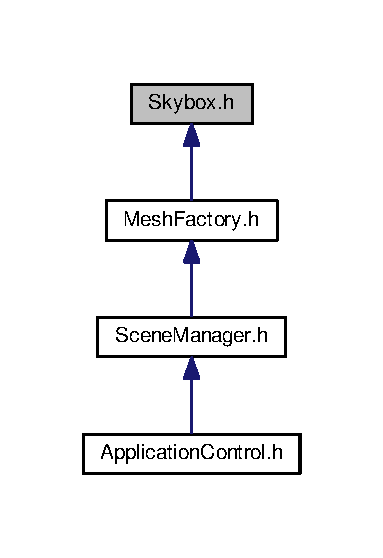
\includegraphics[width=184pt]{Skybox_8h__dep__incl}
\end{center}
\end{figure}
\subsection*{Classes}
\begin{DoxyCompactItemize}
\item 
class \hyperlink{classSkybox}{Skybox}
\begin{DoxyCompactList}\small\item\em Cube avec textures de ciel plaquées. \end{DoxyCompactList}\end{DoxyCompactItemize}


\subsection{Detailed Description}
Simulation d'environnement via skybox monotexturée. 


\hypertarget{SoundManager_8h}{\section{Sound\+Manager.\+h File Reference}
\label{SoundManager_8h}\index{Sound\+Manager.\+h@{Sound\+Manager.\+h}}
}


Définition du gestionnaire de sons.  


{\ttfamily \#include $<$iostream$>$}\\*
{\ttfamily \#include $<$vector$>$}\\*
{\ttfamily \#include $<$string$>$}\\*
{\ttfamily \#include $<$map$>$}\\*
{\ttfamily \#include $<$S\+D\+L2/\+S\+D\+L\+\_\+mixer.\+h$>$}\\*
Include dependency graph for Sound\+Manager.\+h\+:\nopagebreak
\begin{figure}[H]
\begin{center}
\leavevmode
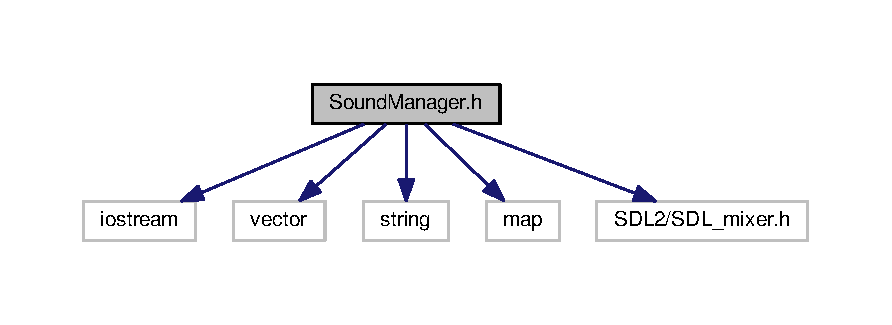
\includegraphics[width=350pt]{SoundManager_8h__incl}
\end{center}
\end{figure}
This graph shows which files directly or indirectly include this file\+:\nopagebreak
\begin{figure}[H]
\begin{center}
\leavevmode
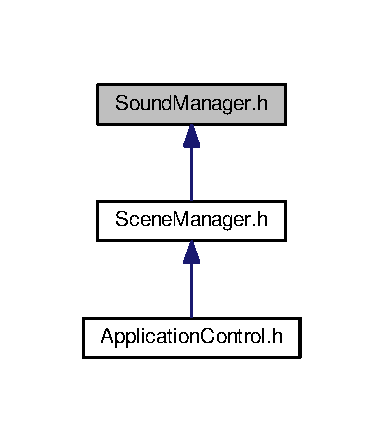
\includegraphics[width=184pt]{SoundManager_8h__dep__incl}
\end{center}
\end{figure}
\subsection*{Classes}
\begin{DoxyCompactItemize}
\item 
class \hyperlink{classSoundManager}{Sound\+Manager}
\begin{DoxyCompactList}\small\item\em Gestionnaire de sons. \end{DoxyCompactList}\end{DoxyCompactItemize}


\subsection{Detailed Description}
Définition du gestionnaire de sons. 


\hypertarget{Sphere_8h}{\section{Sphere.\+h File Reference}
\label{Sphere_8h}\index{Sphere.\+h@{Sphere.\+h}}
}


Implémentation d'une sphère texturée.  


{\ttfamily \#include \char`\"{}Abstract\+Mesh.\+h\char`\"{}}\\*
Include dependency graph for Sphere.\+h\+:\nopagebreak
\begin{figure}[H]
\begin{center}
\leavevmode
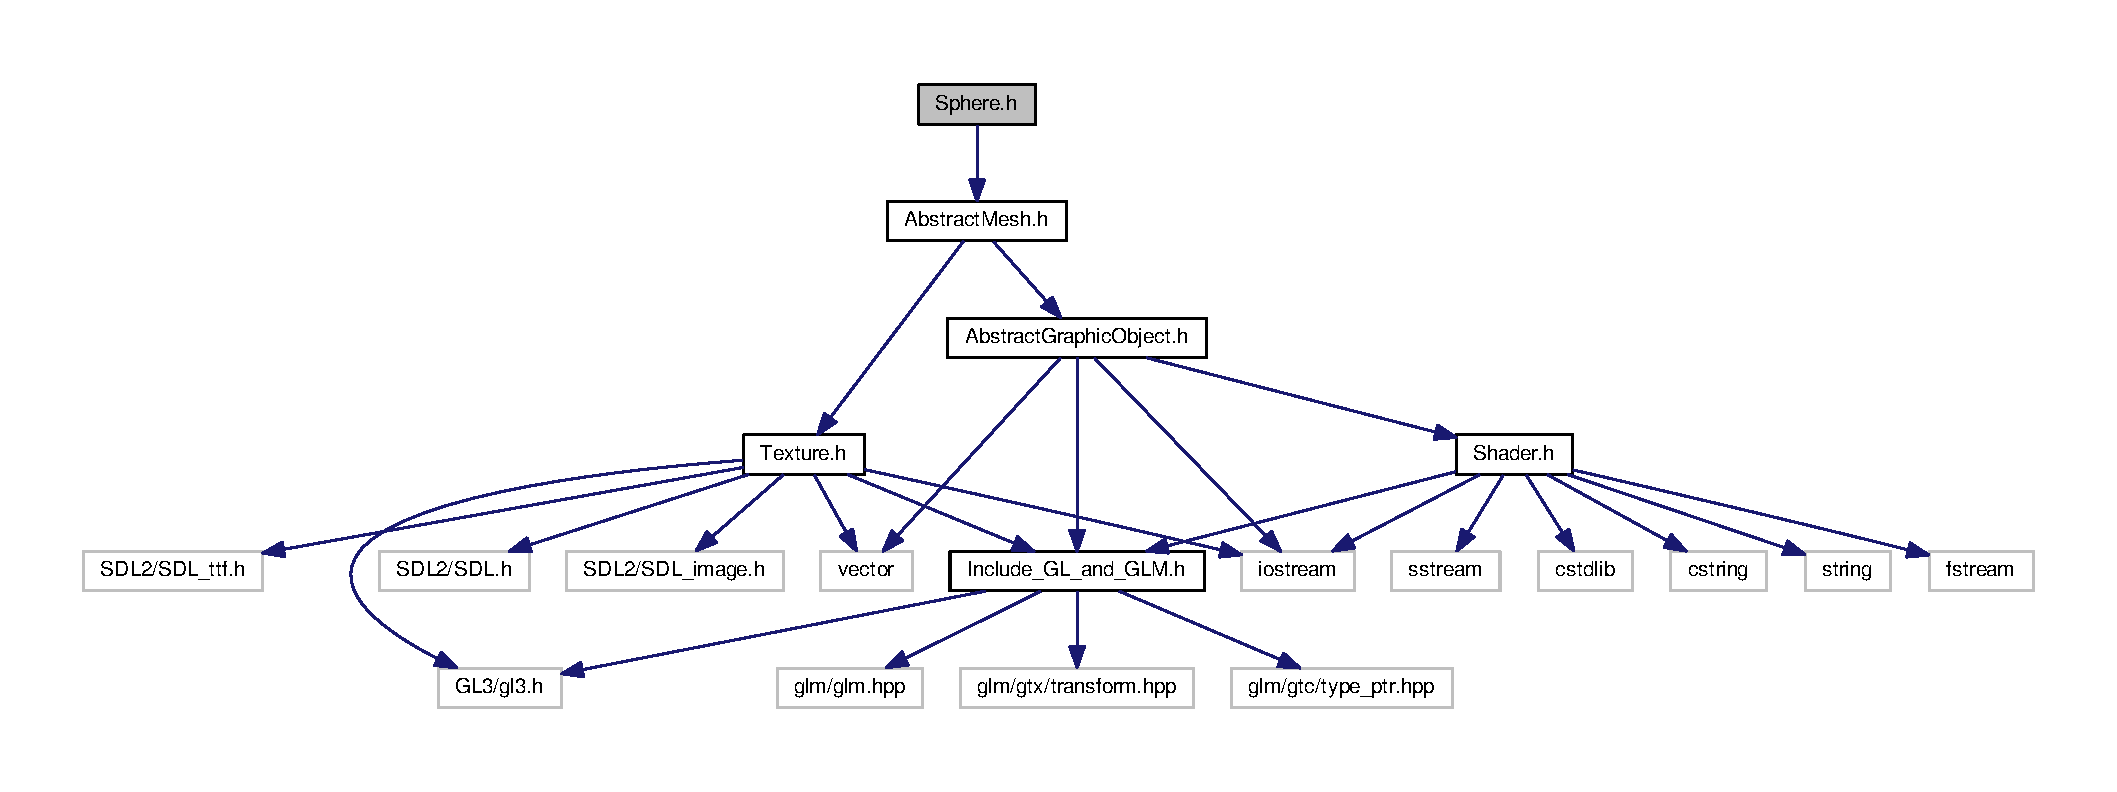
\includegraphics[width=350pt]{Sphere_8h__incl}
\end{center}
\end{figure}
This graph shows which files directly or indirectly include this file\+:\nopagebreak
\begin{figure}[H]
\begin{center}
\leavevmode
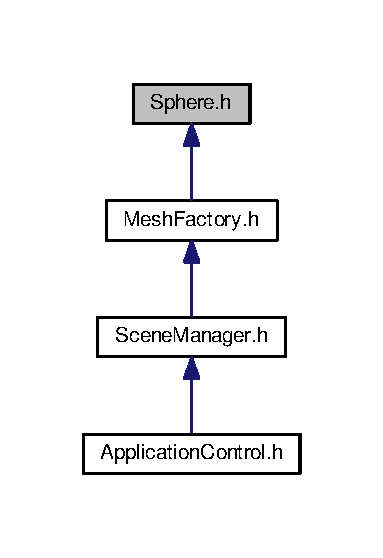
\includegraphics[width=184pt]{Sphere_8h__dep__incl}
\end{center}
\end{figure}
\subsection*{Classes}
\begin{DoxyCompactItemize}
\item 
class \hyperlink{classSphere}{Sphere}
\begin{DoxyCompactList}\small\item\em Définition d'une sphère texturée. \end{DoxyCompactList}\end{DoxyCompactItemize}


\subsection{Detailed Description}
Implémentation d'une sphère texturée. 


\hypertarget{Texture_8h}{\section{Texture.\+h File Reference}
\label{Texture_8h}\index{Texture.\+h@{Texture.\+h}}
}


Gestion des textures.  


{\ttfamily \#include $<$G\+L3/gl3.\+h$>$}\\*
{\ttfamily \#include $<$S\+D\+L2/\+S\+D\+L.\+h$>$}\\*
{\ttfamily \#include $<$S\+D\+L2/\+S\+D\+L\+\_\+image.\+h$>$}\\*
{\ttfamily \#include $<$S\+D\+L2/\+S\+D\+L\+\_\+ttf.\+h$>$}\\*
{\ttfamily \#include \char`\"{}Include\+\_\+\+G\+L\+\_\+and\+\_\+\+G\+L\+M.\+h\char`\"{}}\\*
{\ttfamily \#include $<$iostream$>$}\\*
{\ttfamily \#include $<$vector$>$}\\*
Include dependency graph for Texture.\+h\+:\nopagebreak
\begin{figure}[H]
\begin{center}
\leavevmode
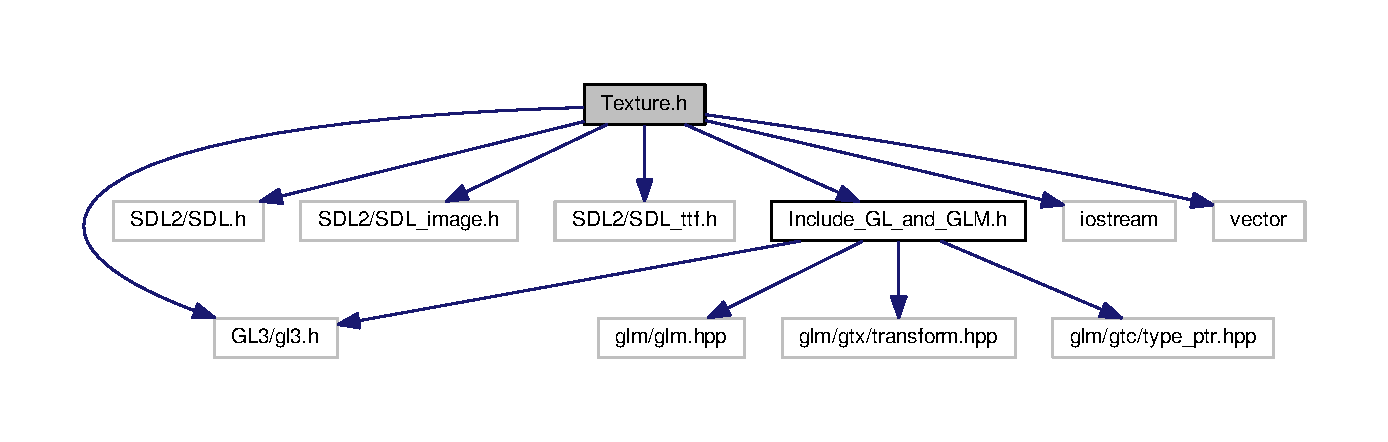
\includegraphics[width=350pt]{Texture_8h__incl}
\end{center}
\end{figure}
This graph shows which files directly or indirectly include this file\+:\nopagebreak
\begin{figure}[H]
\begin{center}
\leavevmode
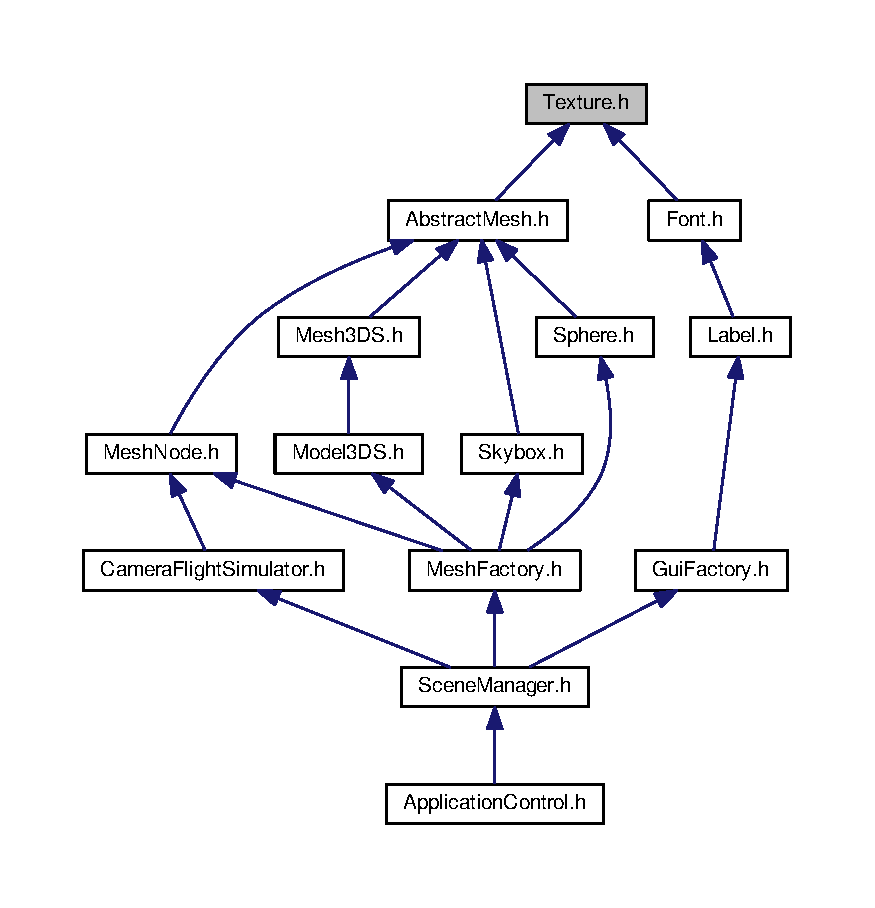
\includegraphics[width=350pt]{Texture_8h__dep__incl}
\end{center}
\end{figure}
\subsection*{Classes}
\begin{DoxyCompactItemize}
\item 
class \hyperlink{classTexture}{Texture}
\begin{DoxyCompactList}\small\item\em Gère les textures Open\+G\+L et leur importation via une image ou une police. \end{DoxyCompactList}\end{DoxyCompactItemize}
\subsection*{Macros}
\begin{DoxyCompactItemize}
\item 
\hypertarget{Texture_8h_a513ae87770898727d346eced6be03bdd}{\#define {\bfseries G\+L3\+\_\+\+P\+R\+O\+T\+O\+T\+Y\+P\+E\+S}~1}\label{Texture_8h_a513ae87770898727d346eced6be03bdd}

\end{DoxyCompactItemize}


\subsection{Detailed Description}
Gestion des textures. 

\begin{DoxyAuthor}{Author}
Raphaël B\+R\+E\+S\+S\+O\+N, Mehdi H\+A\+M\+M\+O\+U\+C\+H\+E 
\end{DoxyAuthor}

%--- End generated contents ---

% Index
\newpage
\phantomsection
\addcontentsline{toc}{chapter}{Index}
\printindex

\end{document}
